\documentclass{article}
\usepackage{fullpage}
\usepackage{color}
\usepackage[normalem]{ulem}
\newcommand{\eric}{\textcolor{blue}{[Eric]}}
\newcommand{\richard}{\textcolor{red}{[Richard]}}
\newcommand{\taylor}{\textcolor{green}{[Taylor]}}
\newcommand{\susi}{\textcolor{cyan}{[Susi]}}
\hyphenpenalty=100000
\usepackage{graphicx}
\DeclareGraphicsExtensions{.pdf,.png,.jpg}
\begin{document}
\setlength{\voffset}{3.5in}
\title{Milestone Master Document}
\author{Team Sriram\\
(Susi Cisneros, Eric Henderson, Taylor Purviance and Richard Thai)}
\date{11 November 2011}
\maketitle
\clearpage
\setlength{\voffset}{0pt}
\tableofcontents
\clearpage
\section{Client Background}
Tim Ekl is a Rose-Hulman graduate student who possesses a significant amount of computer hardware.  He plans on using this system to be able to quickly and easily locate the equipment he wants to use.  Tim is an experienced developer and plans on maintaining the system after it is finished.

\section{Current System}
The client does not have a software solution in place.  Currently, Tim has a primitive categorization system in place which involves labeling boxes and then trying to deduce the location of a desired component.  The current system poses a few issues such as not always allowing him to find his items, i.e. there have been instances where an item was found after capital was spent to replace it.

\section{User/Stakeholder Description}

\subsection{User Profile}
The client will be the main user of the system. While the client is very familiar with sophisticated technologies and software, the final product will be open-source and will be exposed to many more users who will have a broad spectrum of technical proficiency--so the final product will be made with these prospective end users in mind. The client is an accumulator of hardware and disc media, having approximately 1,000 such items which he wants catalogued. Ultimately, identification of the client's items will be based off of a unique identifier, a category, and as many attributes as necessary to describe it.

\subsection{Stakeholder Profiles}

\subsubsection{Stakeholder: Tim Ekl}
\textbf{Role:} Client\\
\textbf{Success:} The final product reasonably satisfies the needs and requirements as defined.\\
\textbf{Failure:} The final product is not easily usable and cannot be extended without major reworking.

\subsubsection{Stakeholder: Team Sriram}
\textbf{Role:} Requirements, Specifications, and Development Team\\
\textbf{Success:} The final product has its requirements defined and prioritized with a satisfactory amount of the high priority features implemented.  The client is able to easily extend and work with the source code provided.\\
\textbf{Failure:} The final product delivered fails to successfully implement the critical features requested by the client.

\subsubsection{Stakeholder: Sriram Mohan}
\textbf{Role:} Class Instructor\\
\textbf{Success:} Team Sriram understood the concepts and processes utilized during the course of the project. The client is satisfied with the final product.\\
\textbf{Failure:} Team Sriram was unable to deduce any concepts or processes discussed during the course. The client is not satisfied with the final product.

\subsection{User Environment}
\begin{itemize}
\item The client uses Chrome whenever possible and prefers that development support Chrome and Firefox browsers.
\item The final product should operate on a Linux server with standard programming languages, programming frameworks, and Apache.  Additional packages can be installed if necessary.
\end{itemize}

\subsection{User Needs}
\begin{tabular}{ | p{0.15in} | p{4.0in} | p{.75in} |}
\hline
\textbf{ID} & \textbf{Need} & \textbf{Priority} \\
\hline
\hline
N0 & Search for parts based off their attributes & Primary \\
\hline
N2 & Identify items via bar codes & Primary \\
\hline
N3 & Keep track of the data associated with an asset & Primary \\
\hline
N4 & Organize search results & Primary \\
\hline
N5 & Insert objects in the system at any point; do not freeze the database & Secondary \\
\hline
N6 & Modify objects; including adding notes to the objects & Secondary \\
\hline
N7 & Access from a second physical location & Optional \\
\hline
N8 & View most-recently acquired asset(s) & Optional \\
\hline
N9 & View a summary of inventory data & Optional \\
\hline
\end{tabular} \\
\textbf{Legend:} \\
Primary - Necessary to the system \\
Secondary - Important to the system \\
Optional - Would be nice to have in the system

\subsection{Alternatives and Competition}
Tim has researched alternative solutions but has not been able to find one that fits his needs.  Alternative systems have been intended for corporate use, are overly complicated, and are designed for large scale use.  Other issues associated with these products include incompatibility with non-Windows environments, excessive cost, and locally restricted access (not accessible through the Internet).  The client has also considered making a system for himself, however he has never had the time to implement it.

\section{Product Overview}

\subsection{Product Perspective}
The software will be an independent system to be hosted on the client's servers.  The product will replace the current solution by electronically keeping track of asset locations. In addition, the software will maintain data associated with each asset.

\subsection{Elevator Statement}
Everyone accumulates items that they currently do not use, but do not want to discard.  Given enough time, a person will accumulate more items than they will be able to consciously track. We propose a web application which will allow for simple and streamlined asset tracking. The software will maintain an organized and systematic inventory which will also keep track of each item's location.

\subsection{Summary of Capabilities}
\begin{tabular}{ | p{4.0in} | p{2.0in} | }
\hline
\textbf{Customer Benefit} & \textbf{Supporting Features}\\
\hline
\hline
Expediently track items based off of specific criteria & F1, F4, F5, F6, F8\\
\hline
View statistics of asset inventory & F4, F7\\
\hline
Keep all data in one place & F0, F2\\
\hline
Access data from anywhere with Internet access & F0\\
\hline
Compatible with the client's current user environment & F9\\
\hline
Change data associated with items & F3\\
\hline
\end{tabular}
\clearpage
\subsection{Assumptions and Dependencies}
\begin{itemize}
\item Availability of network/web hosting.
\item Availability of Ruby [2] and Sinatra [3] framework to run the software.
\item Operates on the Unix operating system.
\end{itemize}

\subsection{Rough Cost Estimate}
Since the solution will be the product of a course project, no monetary capital will be given nor required.  Concerning a time budget, 340 man hours will be invested into the final product (20 hours per week given four team members).

\section{Non-functional Requirements}

\subsection{General}
\begin{itemize}
\item Responsive on the local network.
\item Local/client storage on web browsers using SQLite [5] and Sinatra [3].
\item Allow for easy transfer of inventory data; involves a simple copying, tar'ing, moving, and untar'ing of the directory.
\item Avoid crashing the application or at least handle the crash gracefully; avoid hard server restarts or corruptions.
\end{itemize}

\subsection{Testing}
\begin{itemize}
\item Cucumber [6] is the preferred testing framework. RSpec [7] is recommended if Cucumber [6] is not used.
\item Manually coded unit tests should be used at minimum if no testing framework is utilized.
\end{itemize}

\section{Features}
\subsection{Feature Listing}
\begin{tabular}{ | p{0.15in} | p{2.0in} | p{0.5in} | p{0.5in} | p{0.5in} | p{0.6in} | p{0.5in} | p{0.65in} | }
\hline
\textbf{ID} & \textbf{Feature}\label{feature} & \textbf{Priority}\label{priority} & \textbf{Effort}\label{effort} & \textbf{Risk}\label{risk} & \textbf{Stability}\label{stability} & \textbf{Target Release}\label{target_release} & \textbf{Assigned To}\label{assigned_to} \\
\hline
\hline
F0 & Online UI & Critical & High & High & Low & 1.0 & Eric \\
\hline
F2 & Add assets to the inventory & Critical & Low & High & Low & 1.0 & Richard \\
\hline
F3 & Modify assets in the inventory & Critical & Low & High & Low & 1.0 & Taylor \\
\hline
F4 & The system keeps track of attributes based on category & Critical & Low & High & Low & 1.0 & Susi \\
\hline
F5 & Use a UPC-A barcode as the unique identifier for each asset\label{upc} & Critical & Low & Medium & Low & 1.0 & Eric \\
\hline
F6 & Provide an updated list of recently-added assets & Useful & Medium & Low & Medium & 1.5 & Richard \\
\hline
F7 & Generate reports of asset inventory & Useful & High & Low & Medium & 2.0 & Taylor \\
\hline
F8 & Sort search results based off of barcode, title, and modified / created timestamp & Useful & High & Low & Low & 2.0 & Susi \\
\hline
F10 & Basic search for items based on name or UPC & Critical & High & High & Low & 1.0 & Eric \\
\hline
F11 & Advanced search for items based on all fields related to the item and its category & Critical & High & High & Low & 1.0 & Richard \\
\hline
F12 & Basic and Advanced searches allow the user to include wildcards in the query & Critical & High & High & Low & 1.0 & Taylor \\
\hline
F13 & Basic and Advanced searches will search first by exact / wildcard match, then by fuzzy match & Critical & High & High & Low & 1.0 & Susi \\
\hline
F14 & REST API & Critical & High & High & Low & 1.0 & Eric \\
\hline
\end{tabular}\label{rest}\\ \\ \\
\textbf{Legend:} \\
Critical - Highest importance \\
Important - Medium importance \\
Useful - Lowest importance \\
High / Medium / Low - Degree of a category \\
1.0 - First release of the system \\
1.5 - Next release of the system with significant changes \\
2.0 - Final release of the system \\
~\\
~\\
\subsection{Feature-to-Need Correspondence}
\begin{tabular}{ | c || c | c | c | c | c | c | c | c | c | c | }
\hline
    & N0 & N2 & N3 & N4 & N5 & N6 & N7 & N8 & N9 \\
\hline
\hline
F0  &    &    &    &    &    &    & X  &    &    \\
\hline
F2  &    &    & X  &    & X  &    &    &    &    \\
\hline
F3  &    &    & X  &    &    & X  &    &    &    \\
\hline
F4  &    &    & X  &    & X  & X  &    &    &    \\
\hline
F5  & X  & X  & X  &    &    &    &    &    &    \\
\hline
F6  &    &    &    &    &    &    &    & X  &    \\
\hline
F7  &    &    &    &    &    &    &    &    & X  \\
\hline
F8  & X  & X  &    & X  &    &    &    &    &    \\
\hline
F10 & X  & X  & X  & X  &    &    &    &    &    \\
\hline
F11 & X  & X  & X  & X  &    &    &    &    &    \\
\hline
F12 & X  & X  & X  & X  &    &    &    &    &    \\
\hline
F13 & X  & X  & X  & X  &    &    &    &    &    \\
\hline
F14 &    &    &    &    &    &    & X  &    &    \\
\hline
\end{tabular}

\section{Use Case-to-Feature Correspondence}
\begin{tabular}{ | c || c | c | c | c | c | c | c | c | c | c | c | c | c | c | }
\hline
    & F0 & F2 & F3 & F4 & F5 & F6 & F7 & F8 & F10 & F11 & F12 & F13 & F14 \\
\hline
\hline
UC1  &  X &  X &    &  X &  X &  X &    &    &    &    &    &    &    \\
\hline
UC2  &  X &    &    &    &  X &    &    &  X &  X &    &  X &  X &    \\
\hline
UC3  &  X &    &    &  X &  X &    &    &  X &    &  X &  X &  X &    \\
\hline
UC4  &  X &    &    &  X &  X &    &    &  X &    &    &    &    &    \\
\hline
UC5  &  X &    &    &  X &  X &    &    &    &    &    &    &    &    \\
\hline
UC6  &  X &    &  X &  X &  X &  X &    &    &    &    &    &    &    \\
\hline
UC7  &  X &    &    &  X &  X &    &  X &    &    &    &    &    &    \\
\hline
\end{tabular}\\ \\
NOTE: F14 (REST API feature) is not mapped to a use case because it is not a visible user feature, but still serves as a function if there is an application that attempts to access the system.

\section{Use Cases}
\label{use_case}

\paragraph{Use case syntax}
~\\
Each use case is divided into 8 sections:
\begin{itemize}
\item A ``Basic Description'' section which gives an overview of what functionality the use case demonstrates.
\item An ``Actors'' section to describe who or what interacts with the system in the use case.
\item A ``Pre-conditions'' section which contains the assumptions made, especially those pertaining to the state of the system, prior to the start of the use case.\label{pre_cond}
\item A ``Basic Flow of Events'' section which details the order of events done by the actor(s) and the system under standard conditions. If a particular step in the basic flow has the possibility of failing to occur successfully, one or more alternative flow listings are presented in brackets following the possibility of failure. Each alternative flow listing matches to an alternative flow in the ``Alternative Flow'' section. If a basic flow step fails, the alternative flow that is listed with it is followed as the next step.
\item An ``Alternative Flow of Events'' section which holds each alternative flow listed in the basic flow. Each alternative flow has a unique identifier used to reference it, a short name describing the condition that would cause the alternative flow to be followed, and the order of actions performed by the actor(s) and the system under the flow's conditions. If an action has the possibility of failing, alternatives to that flow are presented just as they are in the basic flow with a reference to the alternative flow to take.
\item A ``Post-conditions'' section which contains guarantees on the result of the use case.\label{post_cond}
\item An ``Extension Points'' section which contains references to other use cases which the completion of the current use case might lead into.
\end{itemize}

\subsection{Add an Item}

\paragraph{Brief Description}
This use case shows the procedure for adding an item to the inventory.

\paragraph{Actors}
\begin{itemize}
\item User
\end{itemize}

\paragraph{Pre-conditions}
\begin{itemize}
\item The current page must have a link to the ``Add Item'' page.
\end{itemize}

\paragraph{Basic Flow of Events}
\begin{enumerate}
\item The user clicks the ``Add Item'' link. [A0]
\item The user fills in the required fields (UPC and Name). [A1]
\item The system dynamically adds the optional attribute fields for the category chosen.
\item The user fills in the appropriate optional attributes and ``Notes'' fields.
\item The user clicks the ``Add Item'' button. [A2]
\item The system adds the item to the inventory database.
\end{enumerate}

\paragraph{Alternative Flows of Events}

\subparagraph{Alternative Flow A0: Server is Down}
\begin{enumerate}
\item The user is notified that the server could not be reached.
\end{enumerate}
\subparagraph{Alternative Flow A1: Required Fields Ommitted}
\begin{enumerate}
\item The user does not fill in the required title or UPC fields.
\item Steps 3, 4, and 5 from the basic flow.
\item The server notifies the user that the required fields were not completed.
\end{enumerate}
\subparagraph{Alternative Flow A2: UPC not Unique}
\begin{enumerate}
\item The system notifies the user that the item cannot be added because the UPC is not unique.
\end{enumerate}

\paragraph{Post-conditions}
\begin{itemize}
\item The user is brought to the home page.
\item The added item is displayed under the ``Recent Changes'' list.
\end{itemize}

\paragraph{Extension Points}
None

\subsection{Basic Search for an Item}

\paragraph{Brief Description}
This use case shows how a basic search from any page  would proceed. This case will encompass the progression from the user entering the search term to the display of the search result(s).

\paragraph{Actors}
\begin{itemize}
\item User
\end{itemize}

\paragraph{Pre-conditions}
\begin{itemize}
\item The current page must have a basic search box.
\end{itemize}

\paragraph{Basic Flow of Events}
\begin{enumerate}
\item The user types a query in the search box.
\item The user clicks the search button.
\item The browser sends a request to the server. [A0]
\item The server queries the database for items entered into the system that match the query. [A1]
\item The server responds with all of the formatted and sorted results of the database query on the same page. [A2]
\item The user is directed to the Advanced Search page with the results of the basic search displayed at the bottom.
\end{enumerate}

\paragraph{Alternative Flows of Events}

\subparagraph{Alternative Flow A0: Empty Query}
\begin{enumerate}
\item The user remains on the current page.
\end{enumerate}

\subparagraph{Alternative Flow A1: Server is Down}
\begin{enumerate}
\item The user is notified that the server could not be reached.
\end{enumerate}

\subparagraph{Alternative Flow A2: No Matches}
\begin{enumerate}
\item The server responds with the message ``No results.''
\item The results page displays the message returned by the server.
\end{enumerate}

\paragraph{Post-conditions}
\begin{itemize}
\item The results page will display the response from the server or that the server was unreachable.
\item The search box will preserve the search term that was originally entered.
\item The results will be prioritized and sorted according to exact matching, then fuzzy matching.
\item The results will be matched using wildcards if they are present in the query.  This will replace the exact matching, and fuzzy matching will then be done on the query with the wildcard characters removed.
\end{itemize}

\paragraph{Extension Points}
\begin{itemize}
\item 5.4 Search Result Sorting
\item 5.5 View Details of an Item
\end{itemize}


\subsection{Advanced Search for an Item}

\paragraph{Brief Description}
This use case shows how a search from the advanced search page  would proceed. This case will encompass the progression from the user entering the search term to the display of the search result(s).

\paragraph{Actors}
\begin{itemize}
\item User
\end{itemize}

\paragraph{Pre-conditions}
\begin{itemize}
\item The current page must be the advanced search page.
\end{itemize}

\paragraph{Basic Flow of Events}
\begin{enumerate}
\item The user chooses a category from a dropdown menu. [A0]
\item The category selection is sent to the server.
\item The server responds with the attribute fields related to the category. [A1]
\item The category's attribute fields are dynamically added to the page.
\item The user optionally fills in the attribute, name, and UPC fields appropriately.
\item The user clicks the search button.
\item The browser sends a request to the server.
\item The server queries the database for items entered into the system that match the query. [A1]
\item The server responds with the formatted and sorted results of the database query. [A3]
\item The list of candidates for the search parameter(s) provided is dynamically added to the bottom part of the page.
\end{enumerate}

\paragraph{Alternative Flow of Events}

\subparagraph{Alternative Flow A0: No Category}
\begin{enumerate}
\item The user fills in the name and/or UPC.
\item Return to basic flow step 6.
\end{enumerate}

\subparagraph{Alternative Flow A1: Server is Down}
\begin{enumerate}
\item The user is notified that the server could not be reached.
\end{enumerate}

\subparagraph{Alternative Flow A2: Empty Query}
\begin{enumerate}
\item The user remains on the current page.
\end{enumerate}

\subparagraph{Alternative Flow A3: No Matches}
\begin{enumerate}
\item The server responds with the message ``No results.''
\item The results page displays the message returned by the server.
\end{enumerate}

\paragraph{Post-conditions}
\begin{itemize}
\item The results page will display the results of the search.
\item The search fields will preserve the search parameter(s) that were originally entered.
\item If appropriate, the results will be prioritized and sorted according to exact matching, then fuzzy matching.
\item The results will be matched using wildcards if they are present in the query.  This will replace the exact matching, and fuzzy matching will then be done on the query with the wildcard characters removed.
\item If completed, the category field will only use exact matching.
\end{itemize}

\paragraph{Extension Points}
\begin{itemize}
\item 5.4 Search Result Sorting
\item 5.5 View Details of an Item
\end{itemize}


\subsection{Search Result Sorting}

\paragraph{Brief Description}
This use case shows how changing the sorting of the items on the search results page would proceed. This case will encompass the progression from the user clicking the sort type link to the display of the search result(s) in the new order.

\paragraph{Actors}
\begin{itemize}
\item User
\end{itemize}

\paragraph{Pre-conditions}
\begin{itemize}
\item The current page must be the search results page.
\end{itemize}

\paragraph{Basic Flow of Events}
\begin{enumerate}
\item The user clicks on a sort type link (options are Name, UPC, Recently Created, and Recently Modified).
\item The browser sends a request to the server.
\item The server queries the database for items entered into the system that match the query. [A0]
\item The server responds with the formatted and sorted results of the database query. [A1]
\item The screen displays to the user a list of candidates for the search parameter(s) provided.
\end{enumerate}

\paragraph{Alternative Flow of Events}

\subparagraph{Alternative Flow A0: Server is Down}
\begin{enumerate}
\item The user is notified that the server could not be reached.
\end{enumerate}

\subparagraph{Alternative Flow A1: No Matches}
\begin{enumerate}
\item The server responds with the message ``No results.''
\item The results page displays the message returned by the server.
\end{enumerate}

\paragraph{Post-conditions}
\begin{itemize}
\item The results page will display the results of the search.
\item The search field(s) will preserve the search parameter(s) that were originally entered.
\item The search fields will be sorted by match method first (wildcard, exact, or fuzzy), then by the selected sort type.
\end{itemize}

\paragraph{Extension Points}
\begin{itemize}
\item 5.5 View Details of an Item
\end{itemize}


\subsection{View Details of an Item}
\paragraph{Brief Description}
This use case shows how a user would select an item from a list to view more detailed information about it.

\paragraph{Actors}
\begin{itemize}
\item User
\end{itemize}

\paragraph{Pre-conditions}
\begin{itemize}
\item The current page must have a link to the item which the user would like to view, as might happen in search results list or the recently modified items list.
\end{itemize}

\paragraph{Basic Flow of Events}
\begin{enumerate}
\item The user clicks on an item (in search results, the recent changes list, or any other place with items listed).
\item The browser queries the server for the item using the UPC code to specify the item.
\item The server responds with all the data stored about the item. [A0]
\item The browser takes the user to a new page with all the data about the item that the server sent.  It is displayed in elements labeled with ``Category:'', ``Size:'', etc. [A1]
\end{enumerate}

\paragraph{Alternative Flow of Events}

\subparagraph{Alternative Flow A0: Server is Down}
\begin{enumerate}
\item The user is notified that the server could not be reached.
\end{enumerate}

\subparagraph{Alternative Flow A1: Item not Found}
\begin{enumerate}
\item The page displays a message saying that the item could not be found.
\end{enumerate}

\paragraph{Post-conditions}
\begin{itemize}
\item The page will display all data about the item that the system currently has logged for the item
\end{itemize}

\paragraph{Extension Points}
\begin{itemize}
\item 5.6 Edit Details of an Item
\end{itemize}

\subsection{Edit Details of an Item}

\paragraph{Brief Description}
This use case shows how a user would modify an item that already exists in the server and save the edited/new field information for future viewing.

\paragraph{Actors}
\begin{itemize}
\item User
\end{itemize}

\paragraph{Pre-conditions}
\begin{itemize}
\item The current page must be an item's detailed description page.
\end{itemize}

\paragraph{Basic Flow of Events}
NOTE: The required fields cannot be unset after creation of the item.  This means that required fields may be changed to any valid and non-empty values.
\begin{enumerate}
\item The user clicks on the value of a field.
\item The page replaces the element with a text field containing the text that was in the element.
\item The user makes the desired changes to the value.
\item The user clicks outside of the field.
\item The browser sends a request to the server asking the value to be changed in the database.
\item The server changes the value in the database. [A0, A1]
\item The server responds that the value was changed.
\item The page changes the text field back into a div element that contains the updated value of the field.
\end{enumerate}

\paragraph{Alternative Flow of Events}

\subparagraph{Alternative Flow A0: Server is Down}
\begin{enumerate}
\item The user is notified that the server could not be reached.
\end{enumerate}

\subparagraph{Alternative Flow A1: Change Unsuccessful}
NOTE: This can happen when the database encounters an error or is not online.
\begin{enumerate}
\item The server responds that the value could not be changed.
\item The page notifies the user that the value could not be changed.
\item The user presses ``Ok'' in the message dialog.
\item The text field is focused again.
\end{enumerate}

\paragraph{Post-conditions}
\begin{itemize}
\item The data on the page will represent the updated state of the data in the system.
\end{itemize}

\paragraph{Extension Points}
None

\subsection{Generate Inventory Report}

\paragraph{Brief Description}
This use case shows the procedure for generating reports of the item inventory.

\paragraph{Actors}
\begin{itemize}
\item User
\end{itemize}

\paragraph{Pre-conditions}
\begin{itemize}
\item The current page must have a link to the ``Generate Report'' page.
\end{itemize}

\paragraph{Basic Flow of Events}
\begin{enumerate}
\item The user clicks the ``Generate Report'' link. [A0]
\item The user is brought to the ``Generate Report'' page.
\item The user chooses the type of report to generate.
\item The user chooses appropriate report fields for the respective option (the options are defined as Master or Category, which will be elaborated on near the completion).
\item The system generates the report accordingly.
\end{enumerate}

\paragraph{Alternative Flows of Events}

\subparagraph{Alternative Flow A0: Server is Down}
\begin{enumerate}
\item The user is notified that the server could not be reached.
\end{enumerate}

\paragraph{Post-conditions}
\begin{itemize}
\item After basic step 5, the user is displayed the report which is generated as specified.
\end{itemize}

\paragraph{Extension Points}
None


\section{Data Flow Diagrams}
\label{dfd}
\paragraph{DFD Legend}
~\\
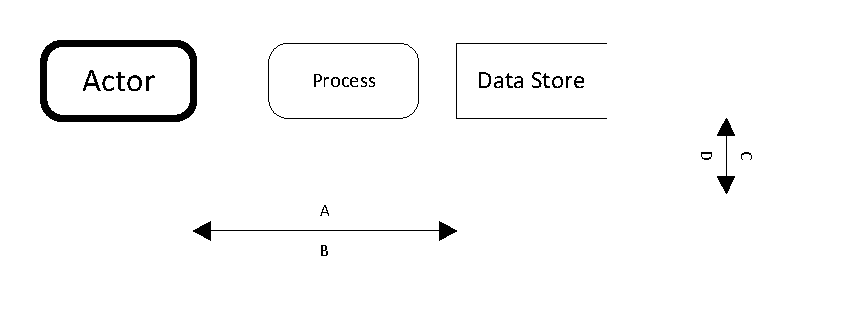
\includegraphics[keepaspectratio, width=4in]{dfd_legend.pdf}\\
\begin{itemize}
\item Actor = some user or another system that interacts with the system.
\item Process = name of some action that will be taken on the data
\item Data Store = something like a file or database that stores data
\end{itemize}
With the bidirectional arrows the data listed above the arrow (like A) flows left-to-right, data listed below the arrow (like B) flows right-to-left, data listed to the right of the arrow (like C) flows top-to-bottom, and data listed to the left of the arrow (like D) flows bottom-to-top.

\paragraph{Context/Level 0}
\label{cfd}
~\\
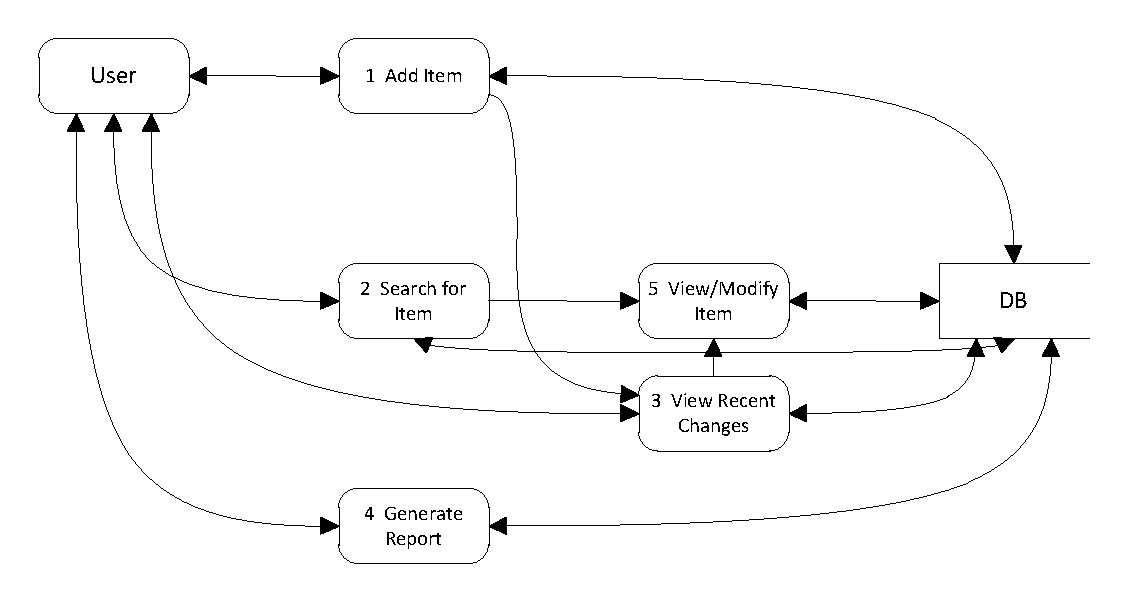
\includegraphics[keepaspectratio, width=6.5in]{dfd_context_level0.pdf}\\
~\\

\paragraph{Level 1: Add Item}
~\\
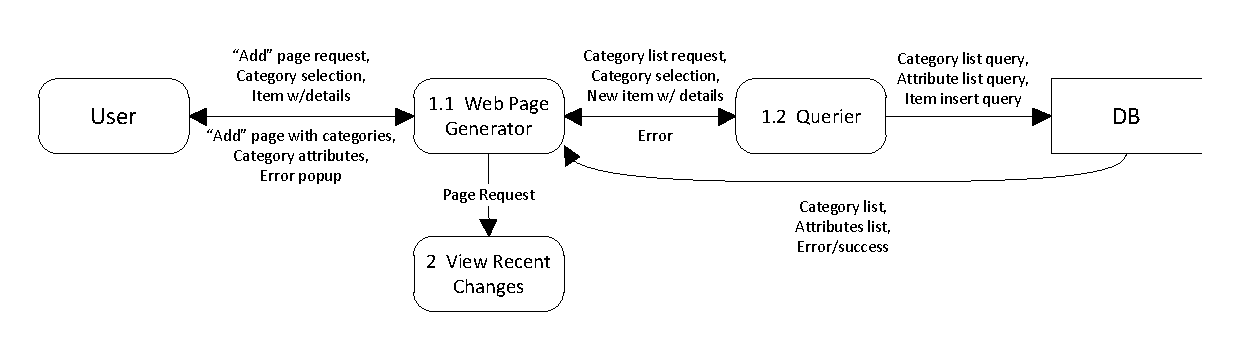
\includegraphics[keepaspectratio, width=6.5in]{dfd_level1_add_item.pdf}\\
~\\

\paragraph{Level 2: Add Item--Querier}
~\\
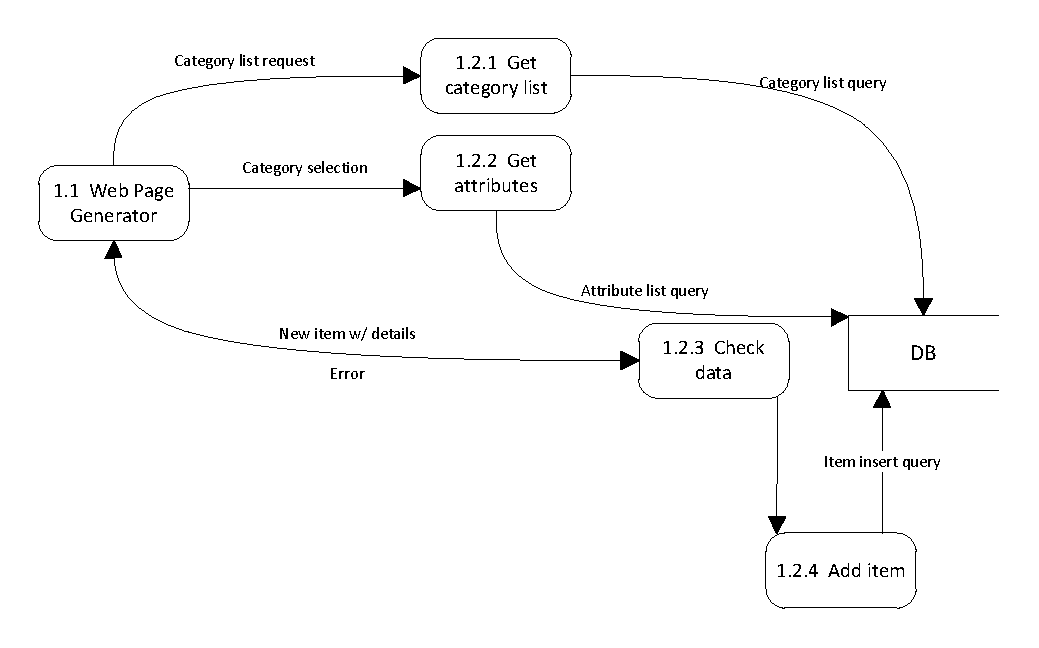
\includegraphics[keepaspectratio, width=6.5in]{dfd_level2_add_item_querier.pdf}\\
~\\

\paragraph{Level 1: Search for Item}
~\\
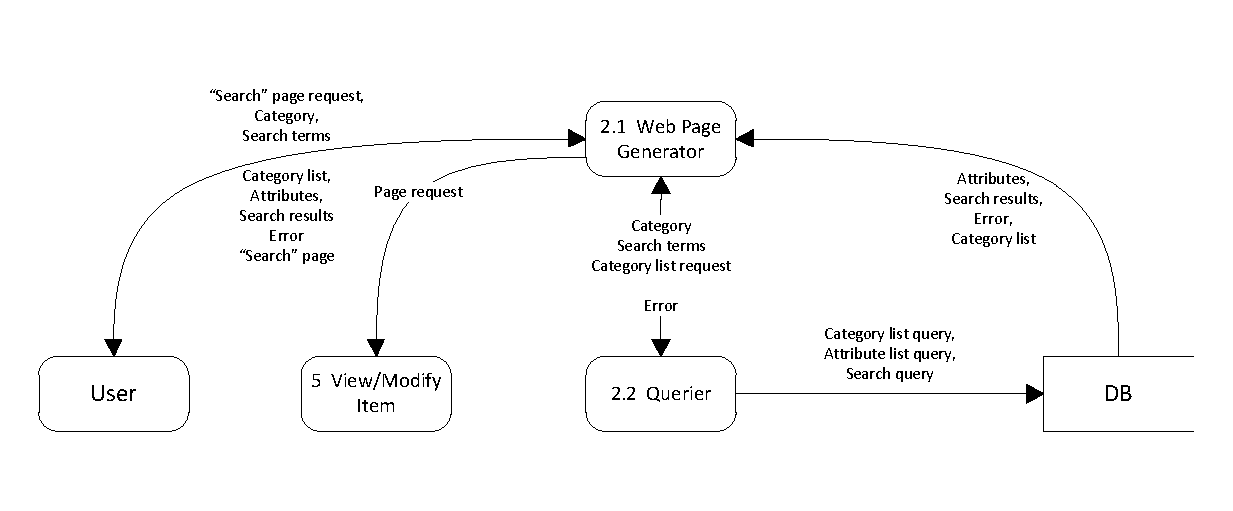
\includegraphics[keepaspectratio, width=6.5in]{dfd_level1_search_for_item.pdf}\\
~\\

\paragraph{Level 2: Search for Item--Querier}
~\\
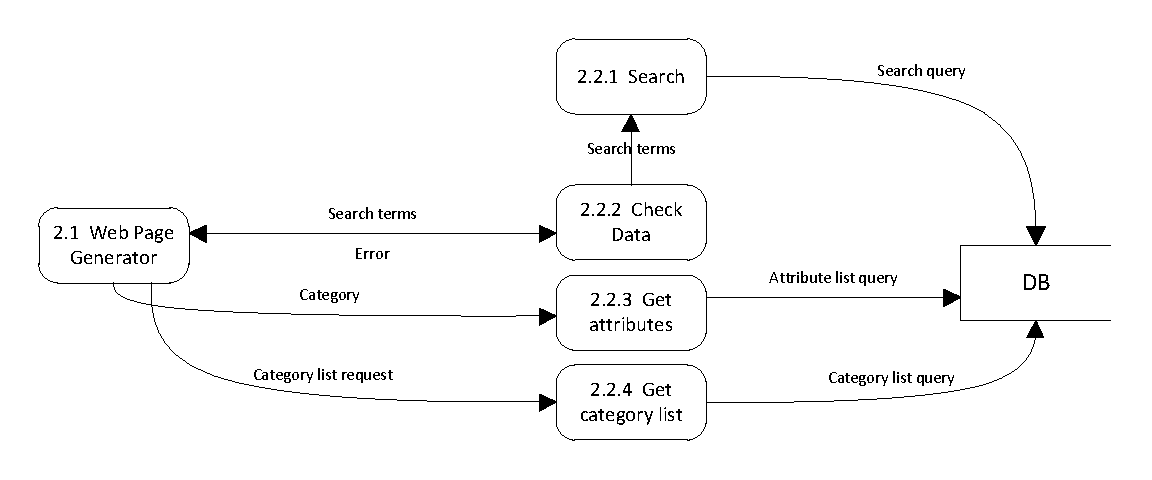
\includegraphics[keepaspectratio, width=6.5in]{dfd_level2_search_for_item_querier.pdf}\\
~\\

\paragraph{Level 1: View Recent Changes}
~\\
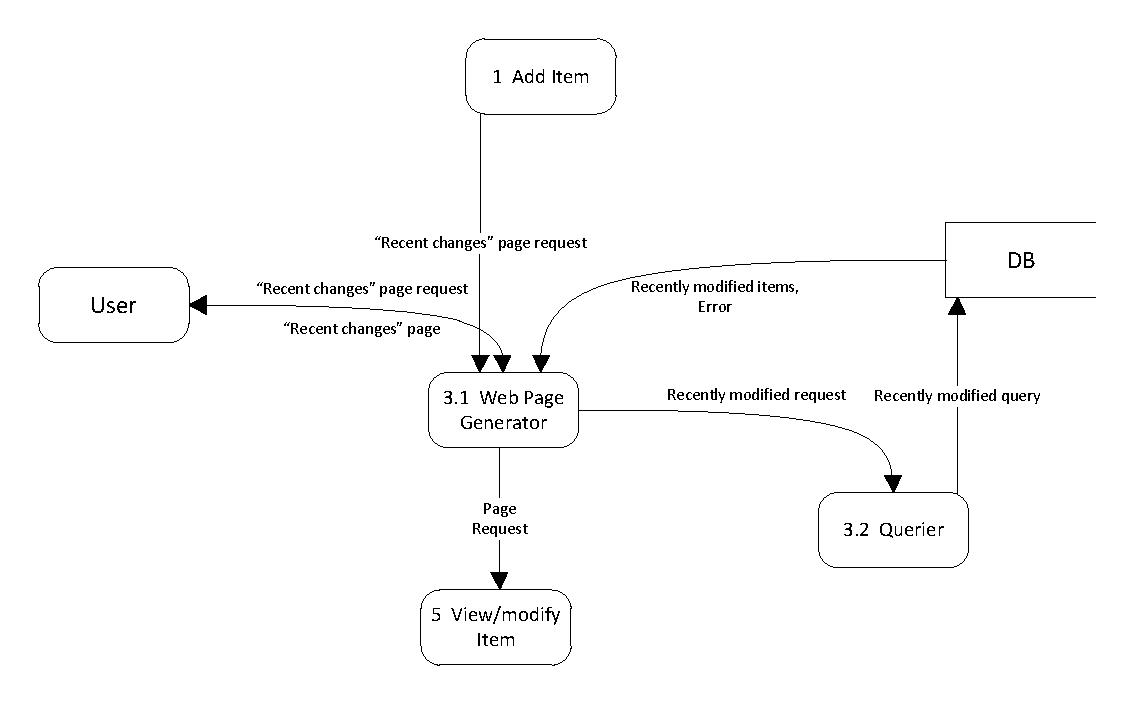
\includegraphics[keepaspectratio, width=6.5in]{dfd_level1_view_recent_changes.pdf}\\
~\\

\paragraph{Level 1: Generate Report}
~\\
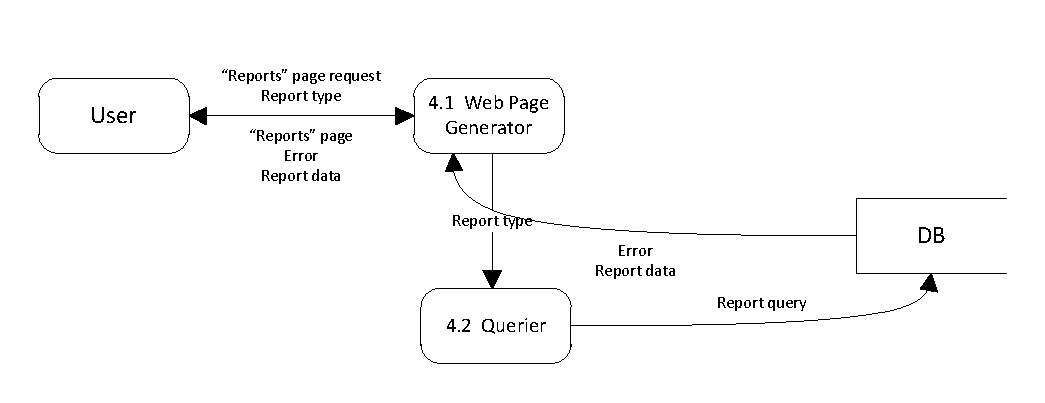
\includegraphics[keepaspectratio, width=6.5in]{dfd_level1_generate_report.pdf}\\
~\\

\paragraph{Level 1: View/Modify Item}
~\\
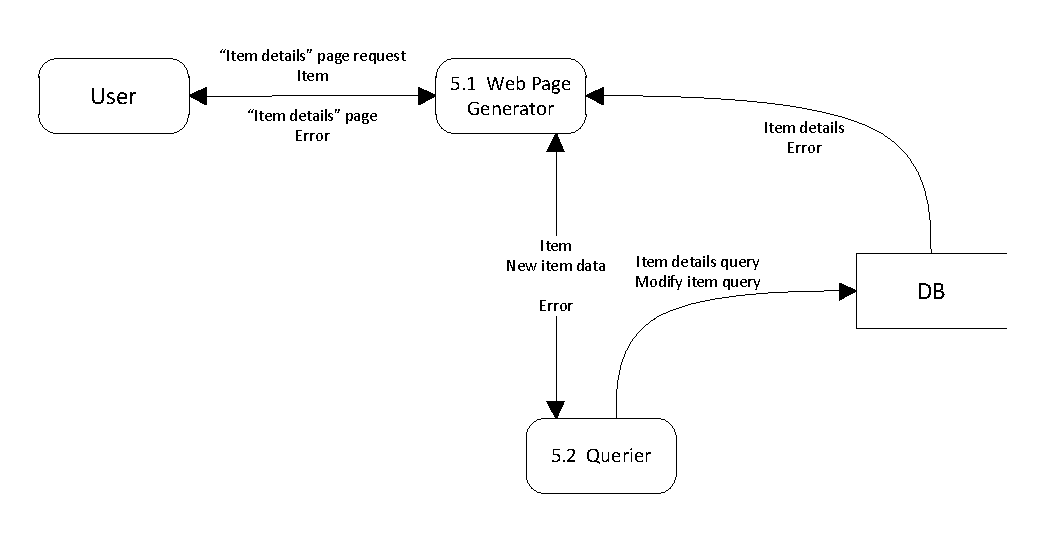
\includegraphics[keepaspectratio, width=6.5in]{dfd_level1_view_modify_item.pdf}\\
~\\

\paragraph{Level 2: View/Modify Item--Querier}
~\\
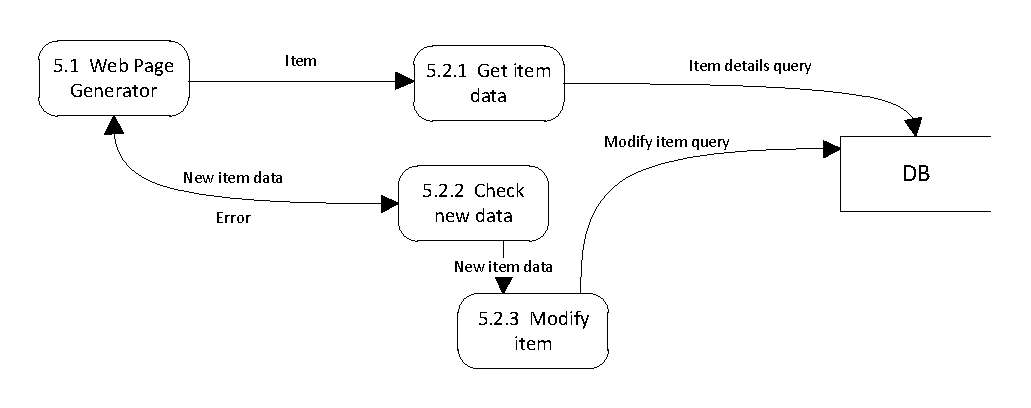
\includegraphics[keepaspectratio, width=6.5in]{dfd_level2_view_modify_item_querier.pdf}\\
~\\

\section{Usability Requirements}
\label{usability}
\begin{itemize}
\item User should be able to familiarize himself or herself with the software within one hour
\item An online help system / documentation will not be required
\item Since the client is not greatly concerned with the usability of the product, there will be very relaxed criteria concerning this aspect.  As such, if the client has any issues with usability of the product, the client will request the change or implement it on his own time, depending on the constraints of the development team.
\end{itemize}

\section{Performance Requirements}
\label{performance}
NOTE: Any times described in the Performance Requirements are based on the client's machine specifications, which are: Pentium 4 2.8GHz processor with 1.5GB memory.
\begin{itemize}
\item Searches should take no longer than three seconds
\item There should be no noticeable (as judged by the client) difference in search performance (the most complex task) between 10 items and 1000 items
\item There is no tolerance for any system degradation: the system is either fully functional or not functional at all, and there is no need to handle failures.\label{degrad_sys}
\end{itemize}

\section{Reliability Requirements}
\label{reliability}
\begin{itemize}
\item The system should not be down more than once every two months
\item The system repair will be the responsibility of the client after the product is delivered
\item The system must have no data corruption (100\% accuracy)\label{data_corruption}
\item The system will have no more than two bugs per thousand lines of code\label{bug}
\item The system should minimize the number of critical bugs, though there is no defined threshold
\end{itemize}

\section{Supportability Requirements}
\label{support}
\begin{itemize}
\item The system will be able to be supported by open source community and the client
\item The source code needs to be kept clean and easy to understand
\item The source code will follow Ruby coding standards and naming conventions
\item The client should be able to extend the system with features of moderate complexity within four hours; this is an intended effect from following the Ruby coding standards
\item The source code should be as modular as possible in order to simplify extension
\item Adding / modifying an API route should as difficult as adding / modifying a web application feature of equal complexity
\end{itemize}

\section{Hardware and Software Interfaces}
The final product will utilize and / or be compatible with the following software products:\\
\begin{itemize}
\item Ruby 1.9.2 [2]
\item Sinatra 1.3.0 [3]
\item Ubuntu 11.04 [4]
\item SQLite 3.7.8 [5]
\item Cucumber 1.1.0 [6]
\item RSpec 2.6.0 [7]
\item DataMapper 1.1.0 [8]
\item Google Chrome 14.0.8 [9]
\item Firefox 7.0.1 [10]
\item Apache 2.2 [11]
\end{itemize}

\section{Documentation, Installation, Legal, and Licensing Requirements}
\begin{itemize}
\item The project should be open source, distributed under the BSD license
\item Copyright ownership will be given to the client
\item Installation should only require installing the necessary packages and pulling the code from the Git repository into the web server directory
\item The only documentation necessary is a simple readme as well as comments near complex sections of code
\end{itemize}

\section{Design Constraints}
\begin{itemize}
\item The project must be open source
\item The project must be completed within five months
\item The project must be completed without funding from the client
\item The project must utilize REST, not SOAP\label{soap}
\item Develop in Ruby utilizing Sinatra for web framework
\item Accessible via the web.
\end{itemize} 

\section{User Interfaces}
\graphicspath{{../StoryboardImages/}}
~\\
\begin{tabular}{ p{4.5in} }
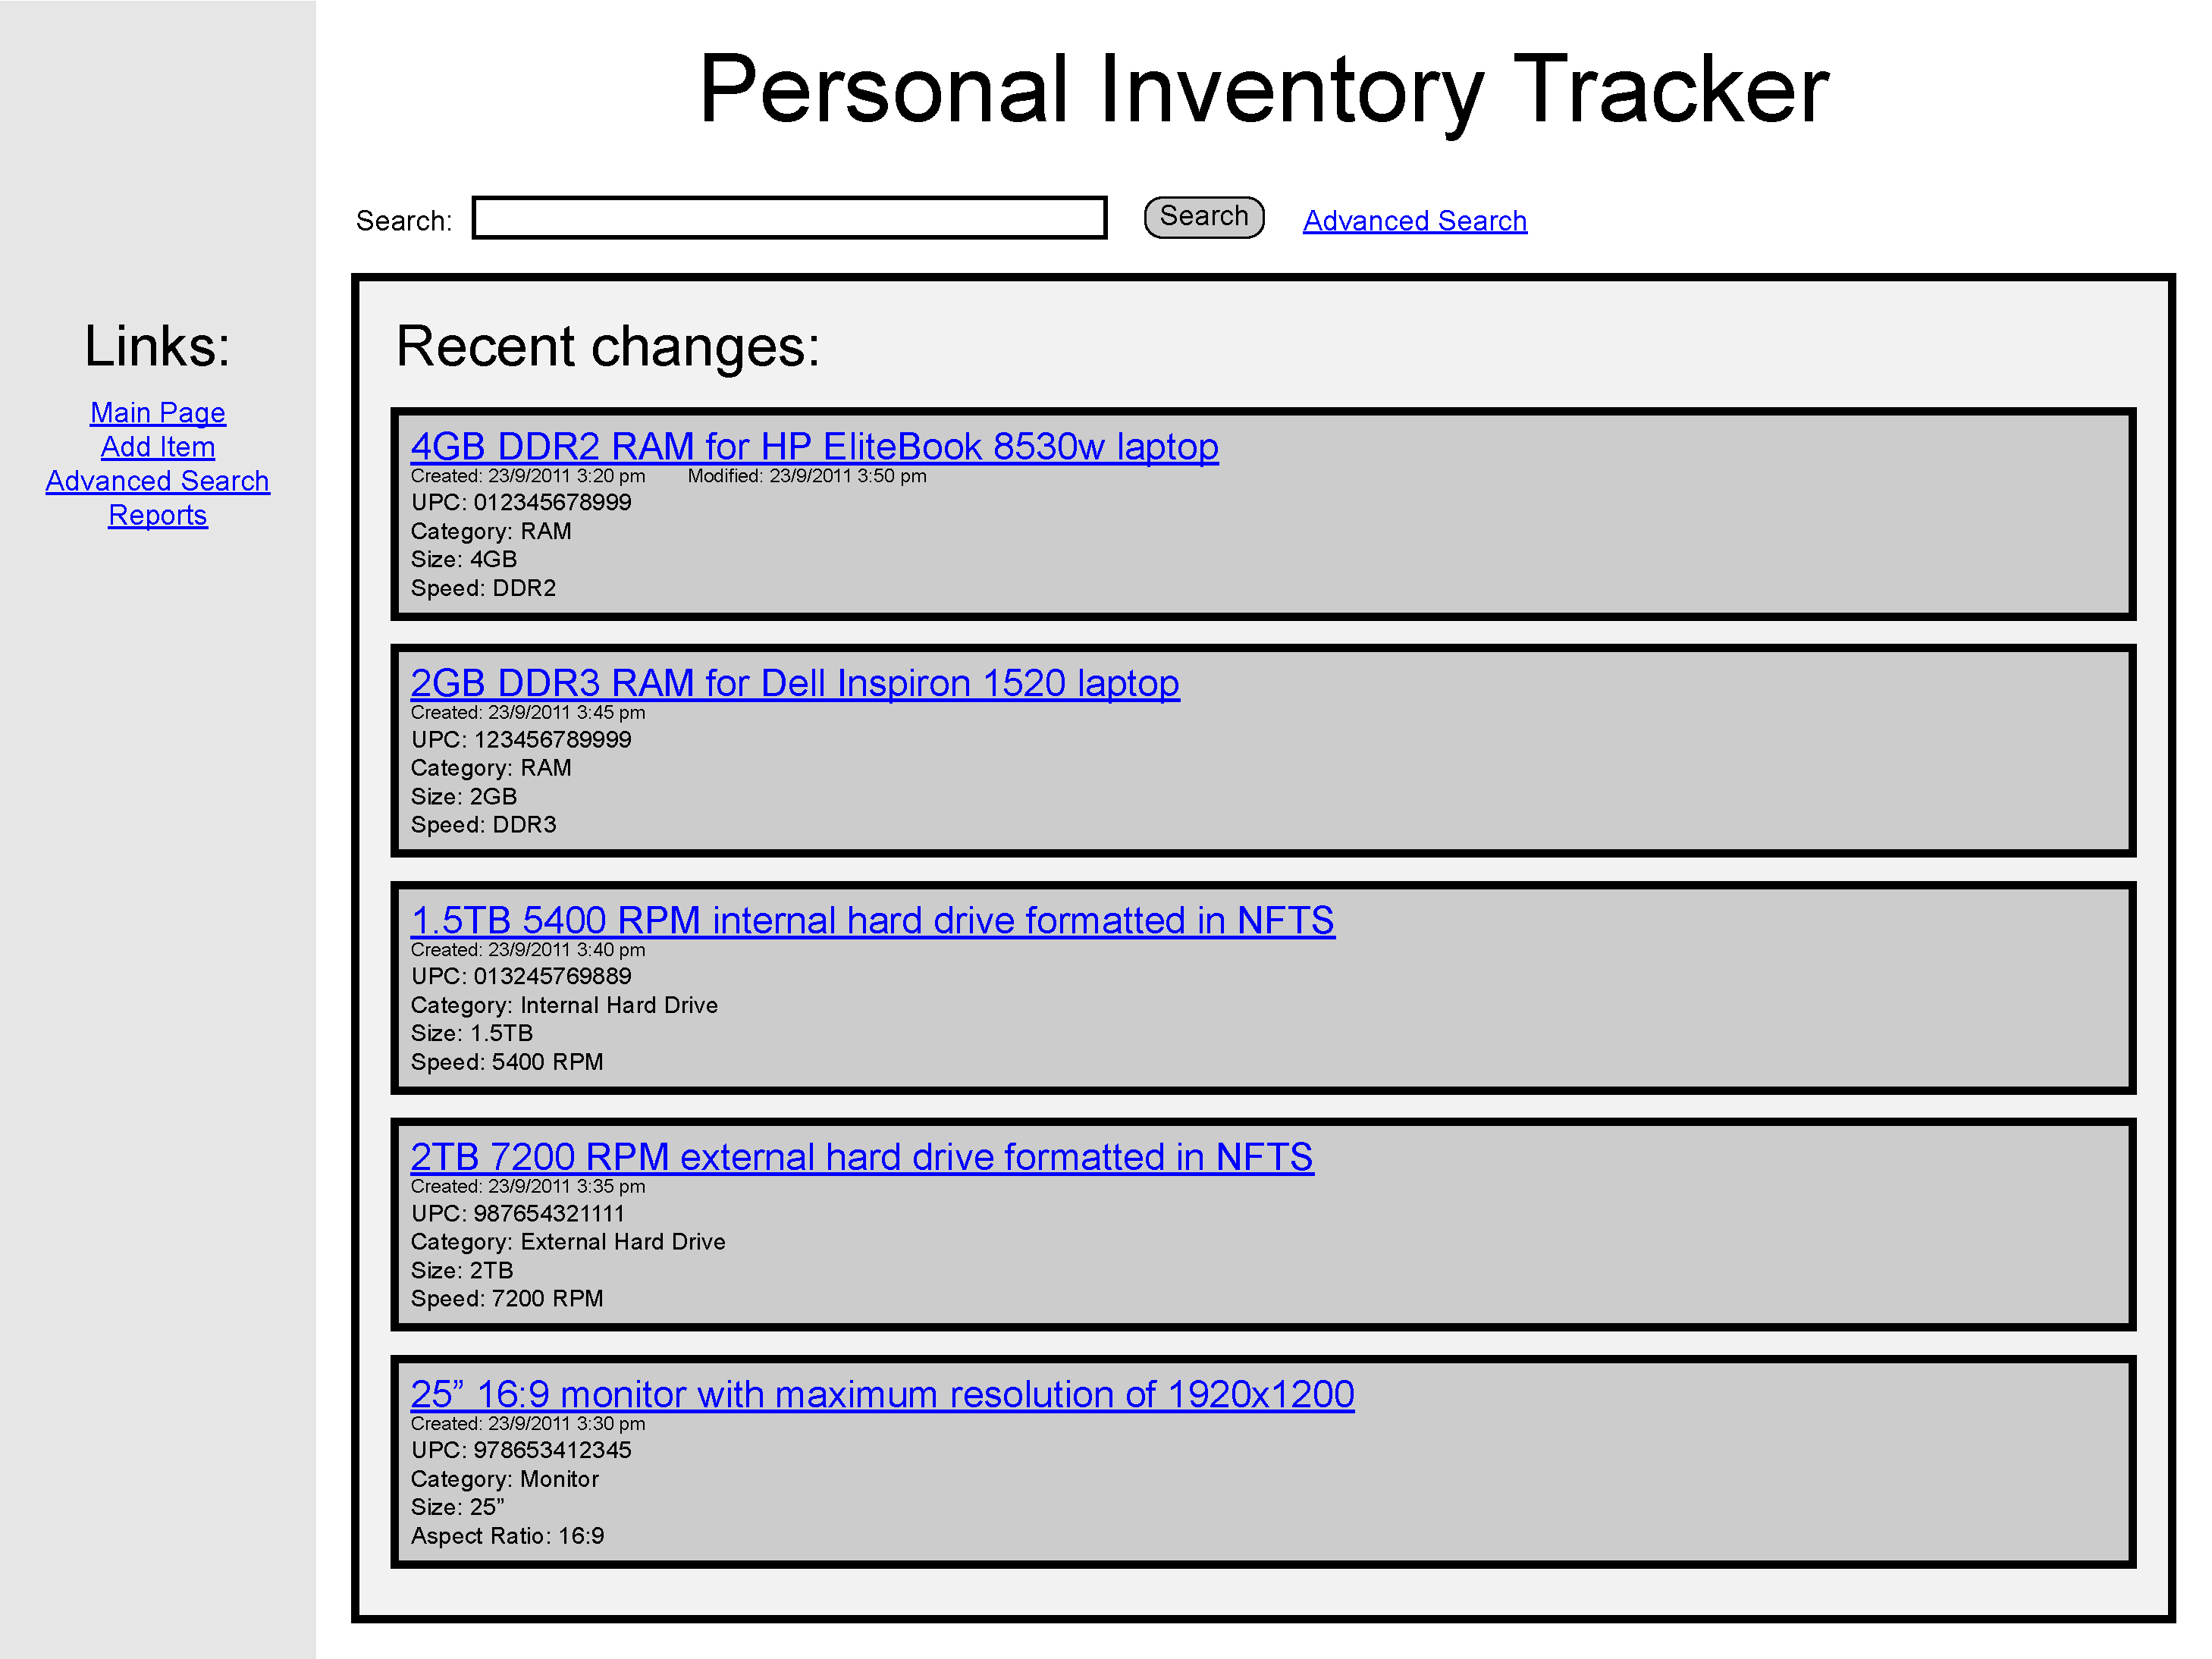
\includegraphics[keepaspectratio, width=4.5in]{addItemF0S0.pdf}\\
The main page, showing no more than the top five most recent changes: a design aspect requested by the client
\end{tabular}\\
~\\
~\\
\begin{tabular}{ p{4.5in} }
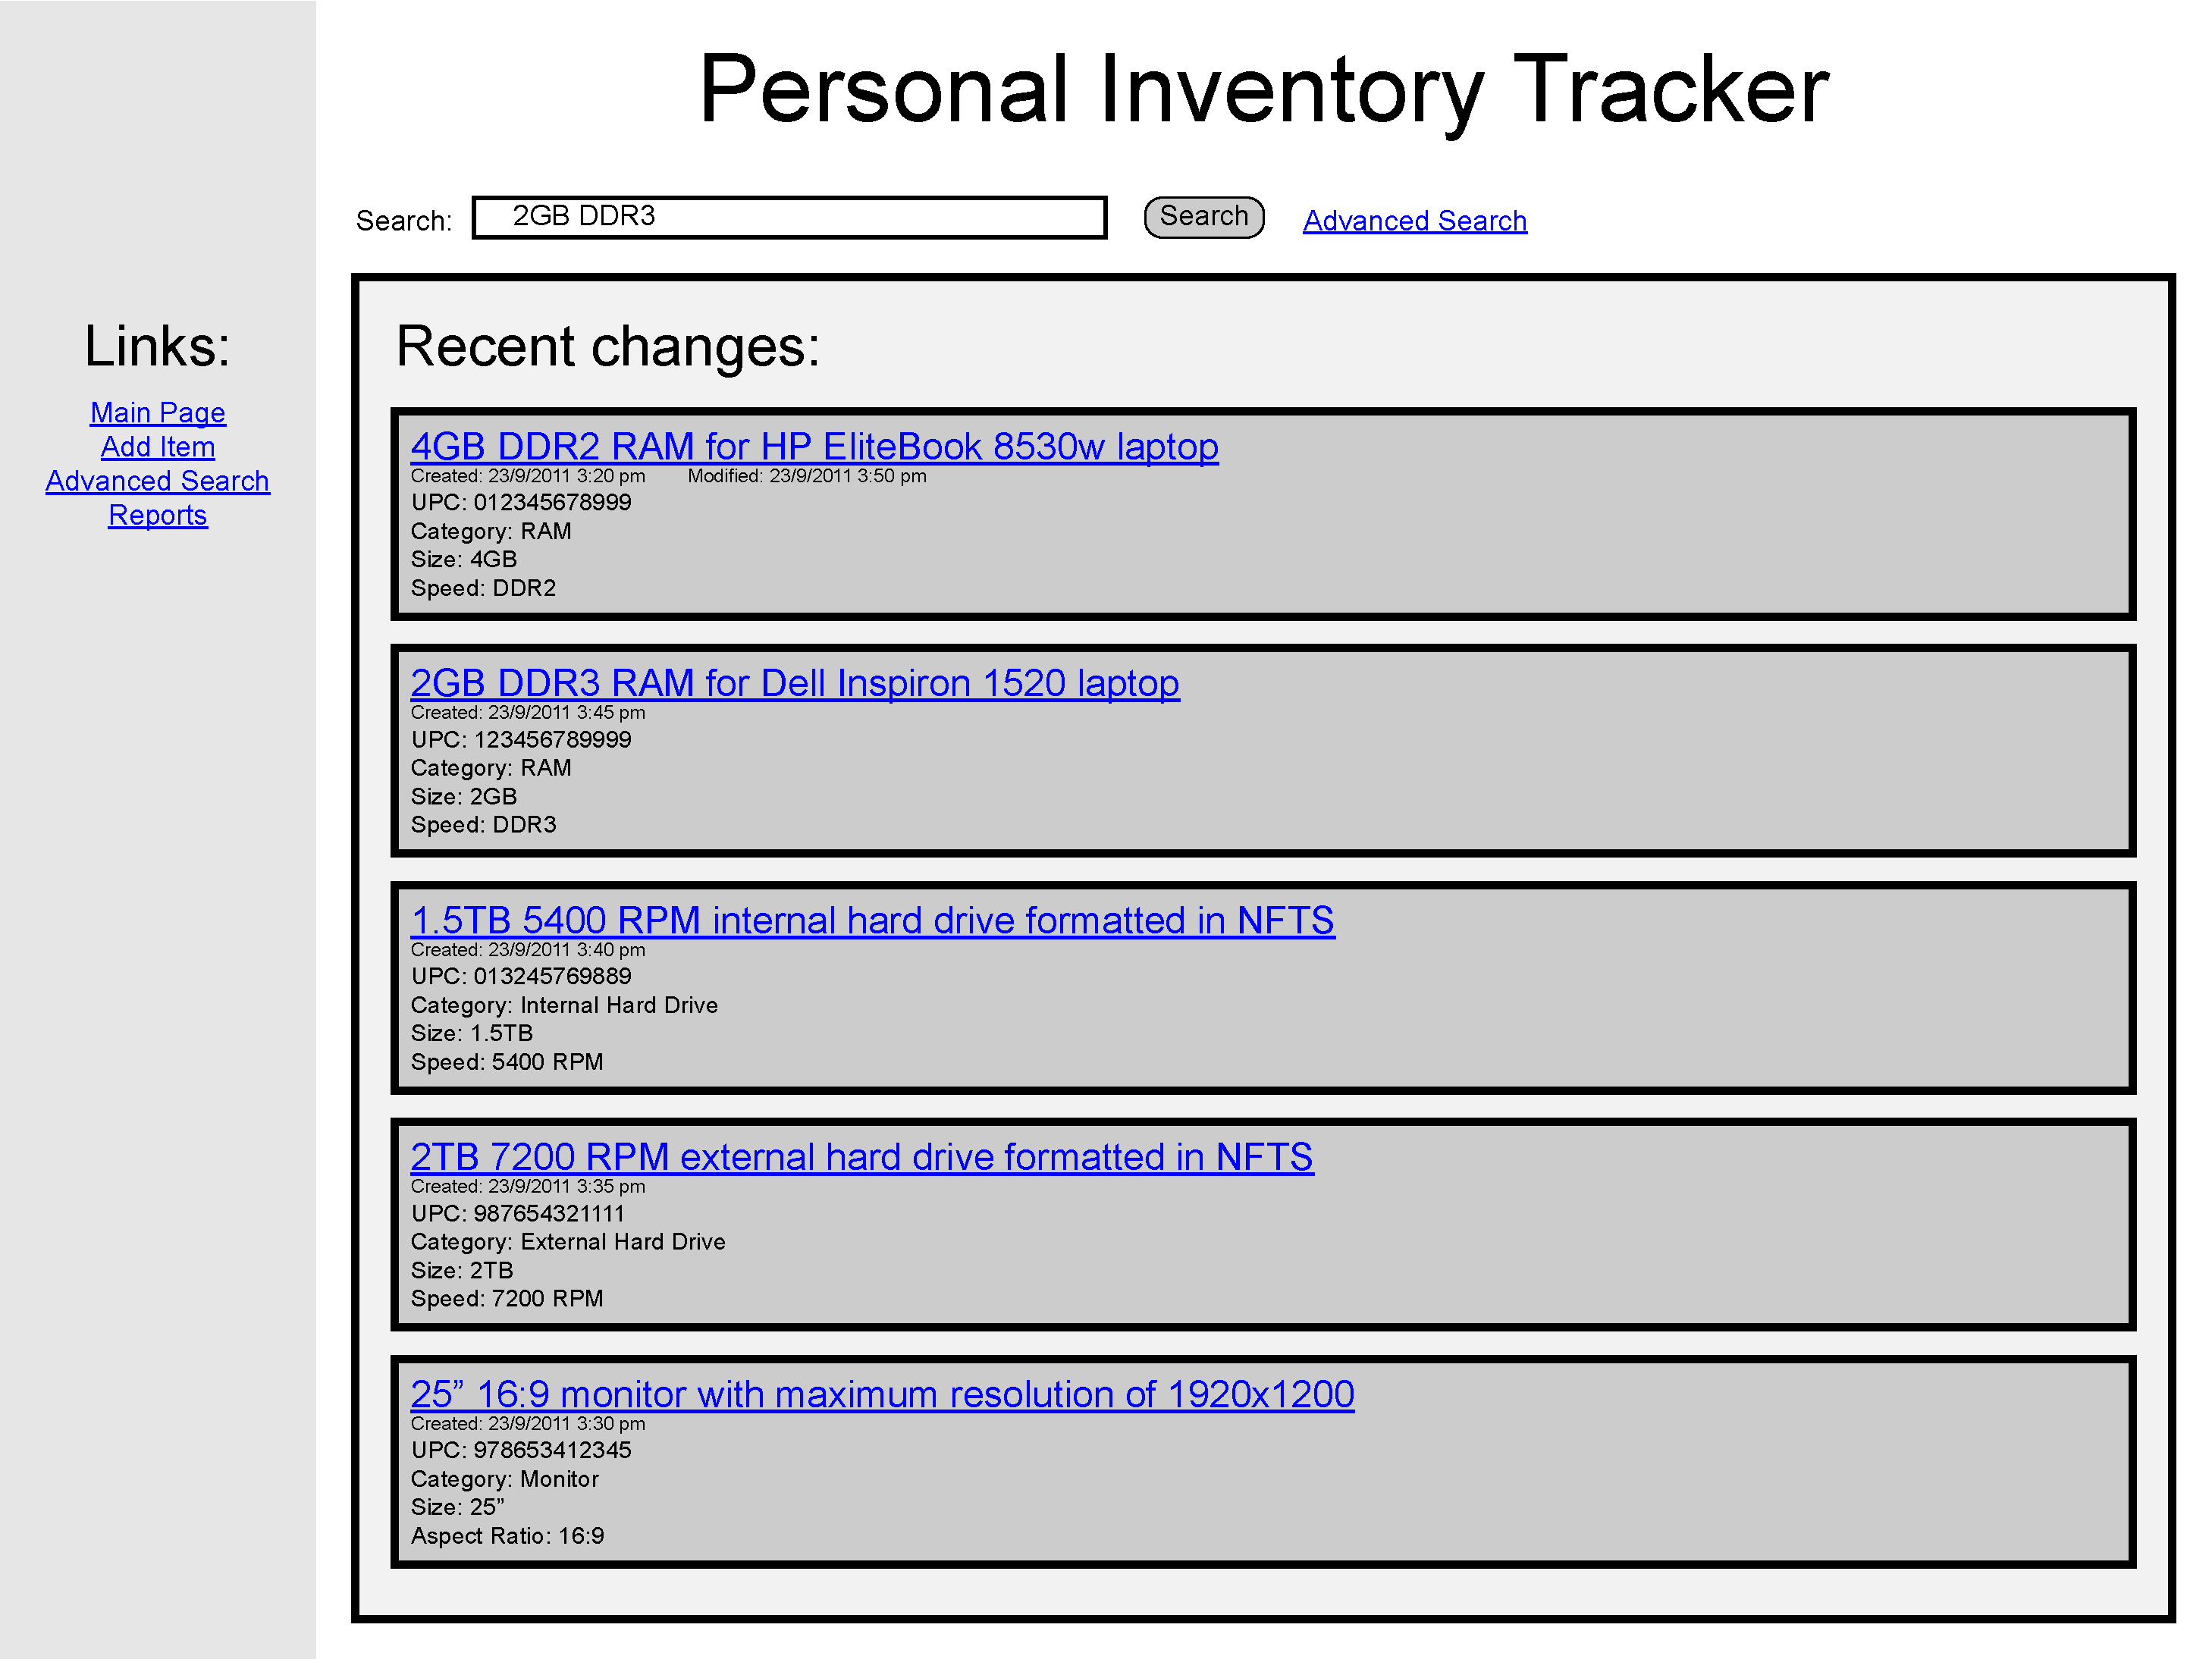
\includegraphics[keepaspectratio, width=4.5in]{basicSearchF0S0.pdf} \\
The main page with a basic search query filled in
\end{tabular}\\
~\\
~\\
\begin{tabular}{ p{4.5in} }
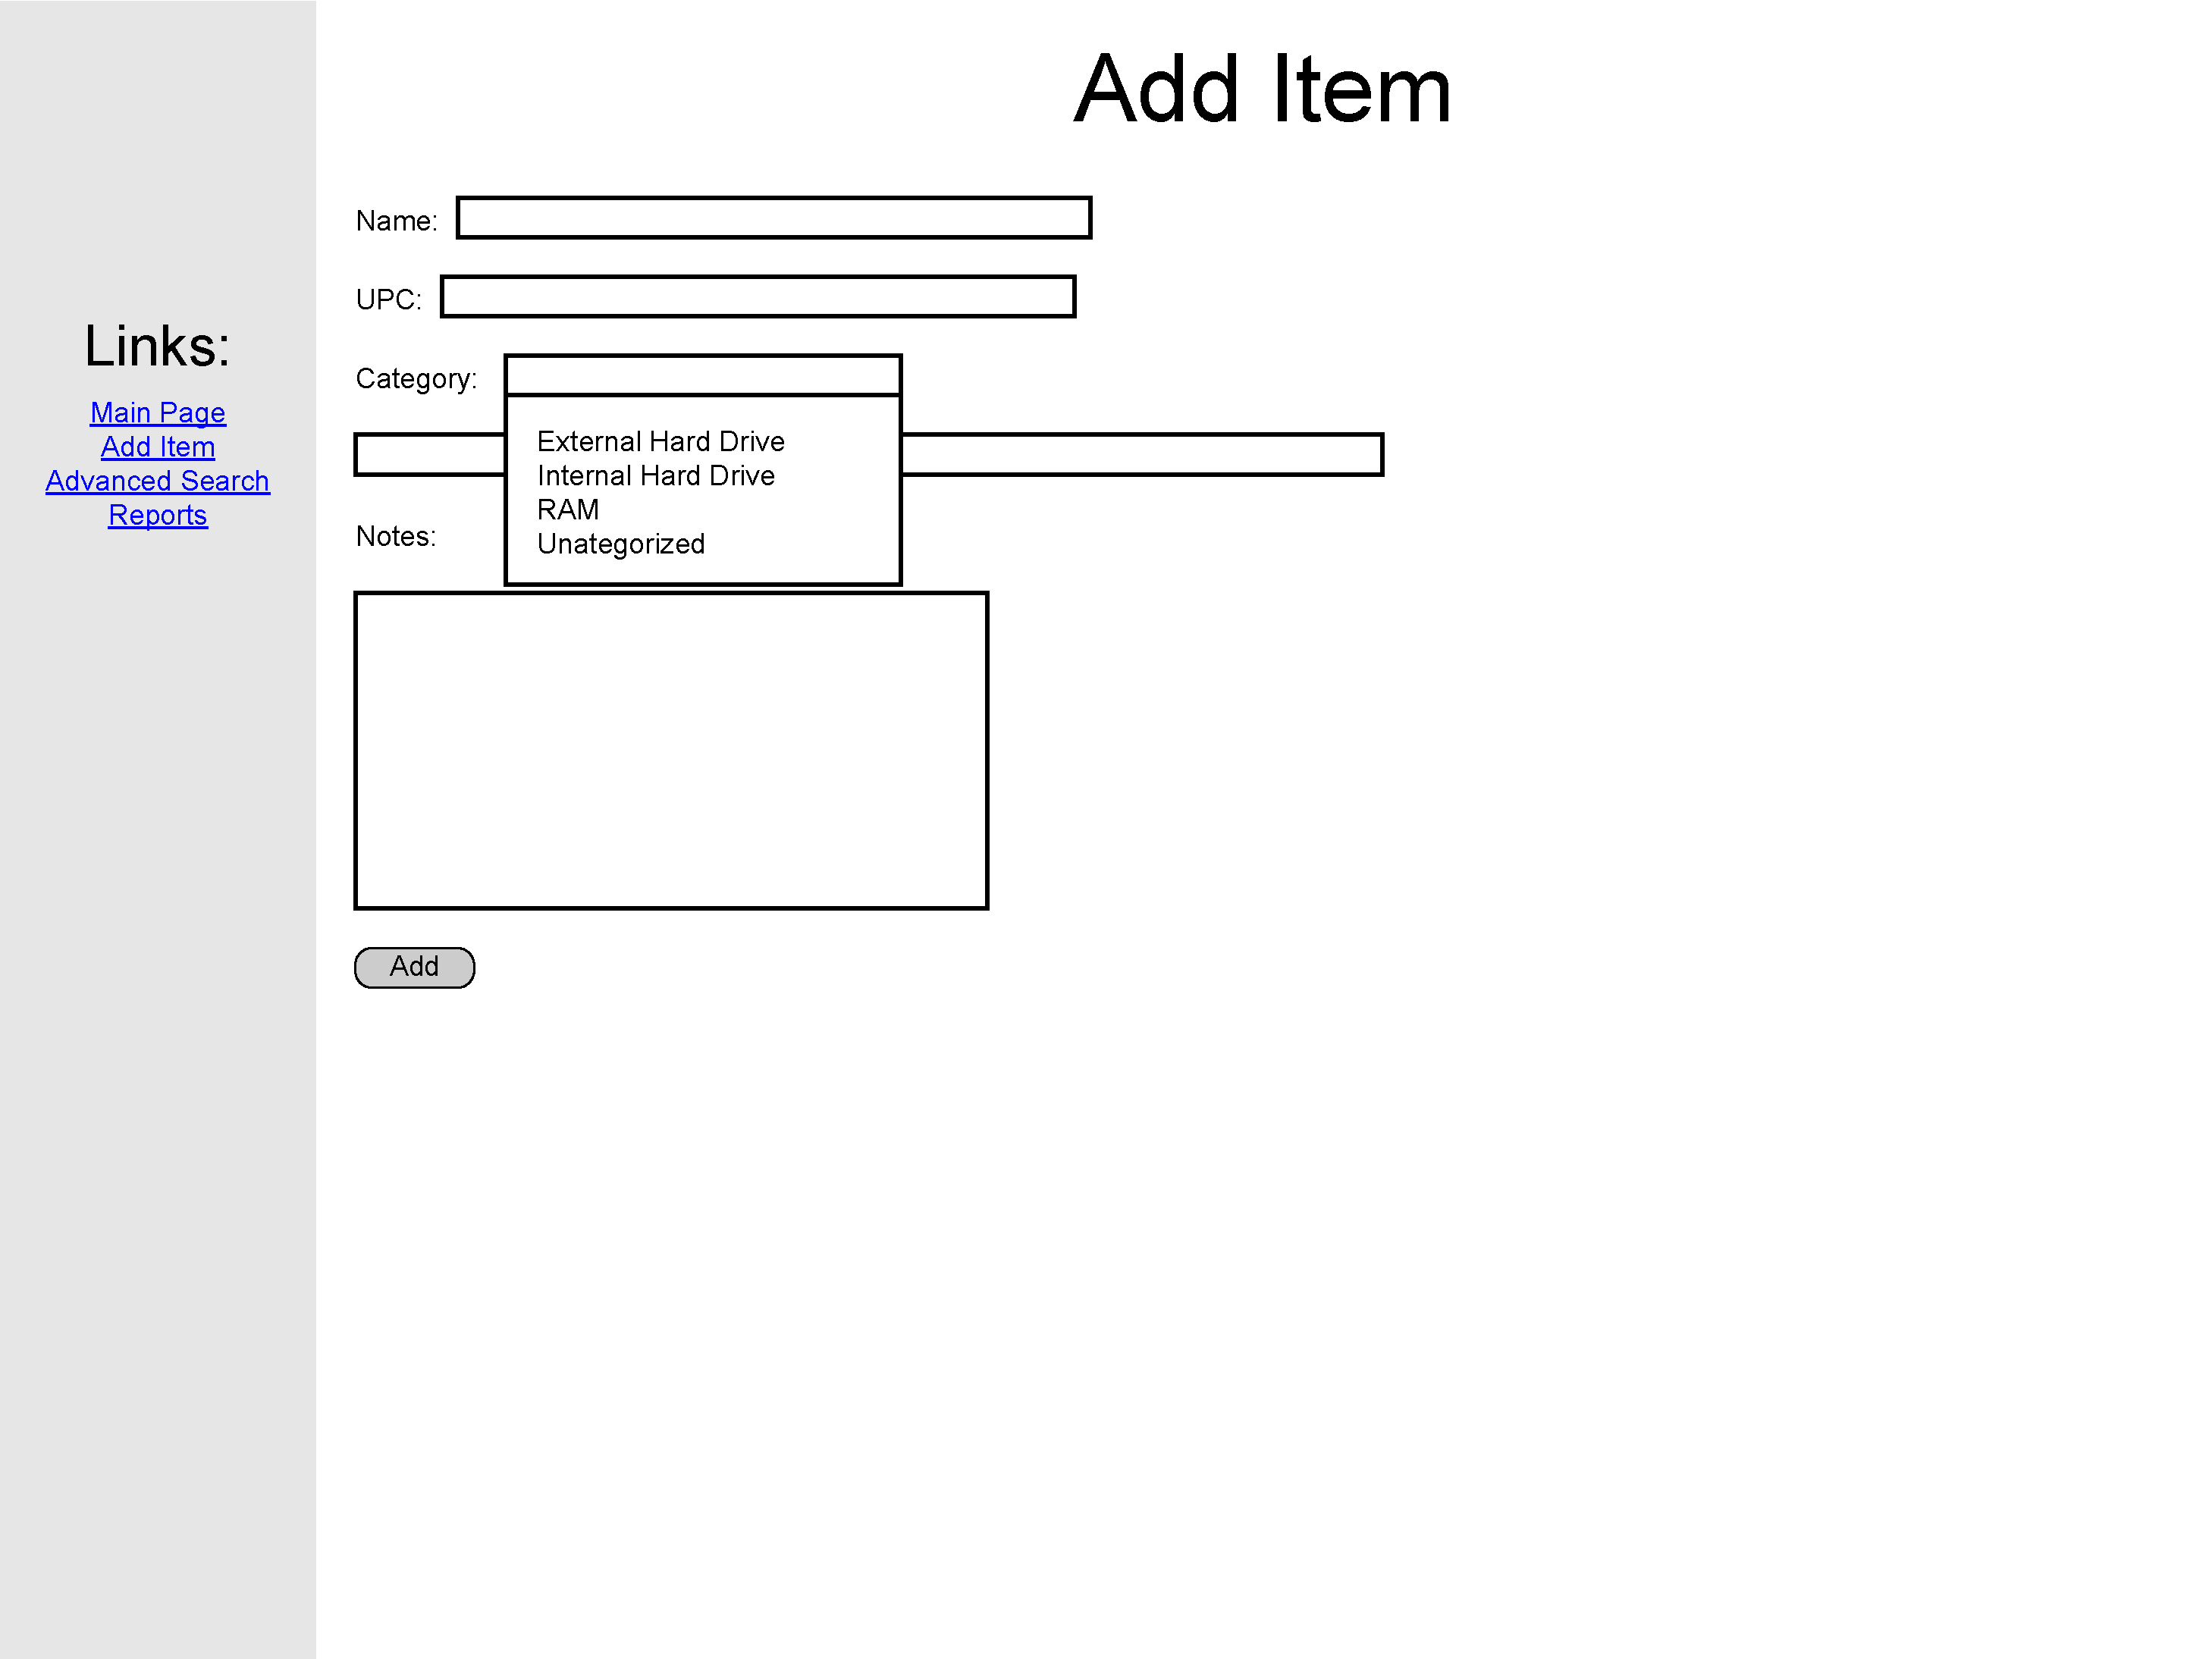
\includegraphics[keepaspectratio, width=4.5in]{addItemF0S1.pdf}\\
The add item page with category autocomplete showing.  The Name and UPC fields are required to be non-empty (and in the case of UPCs, unique as well).
\end{tabular}\\
~\\
~\\
\begin{tabular}{ p{4.5in} }
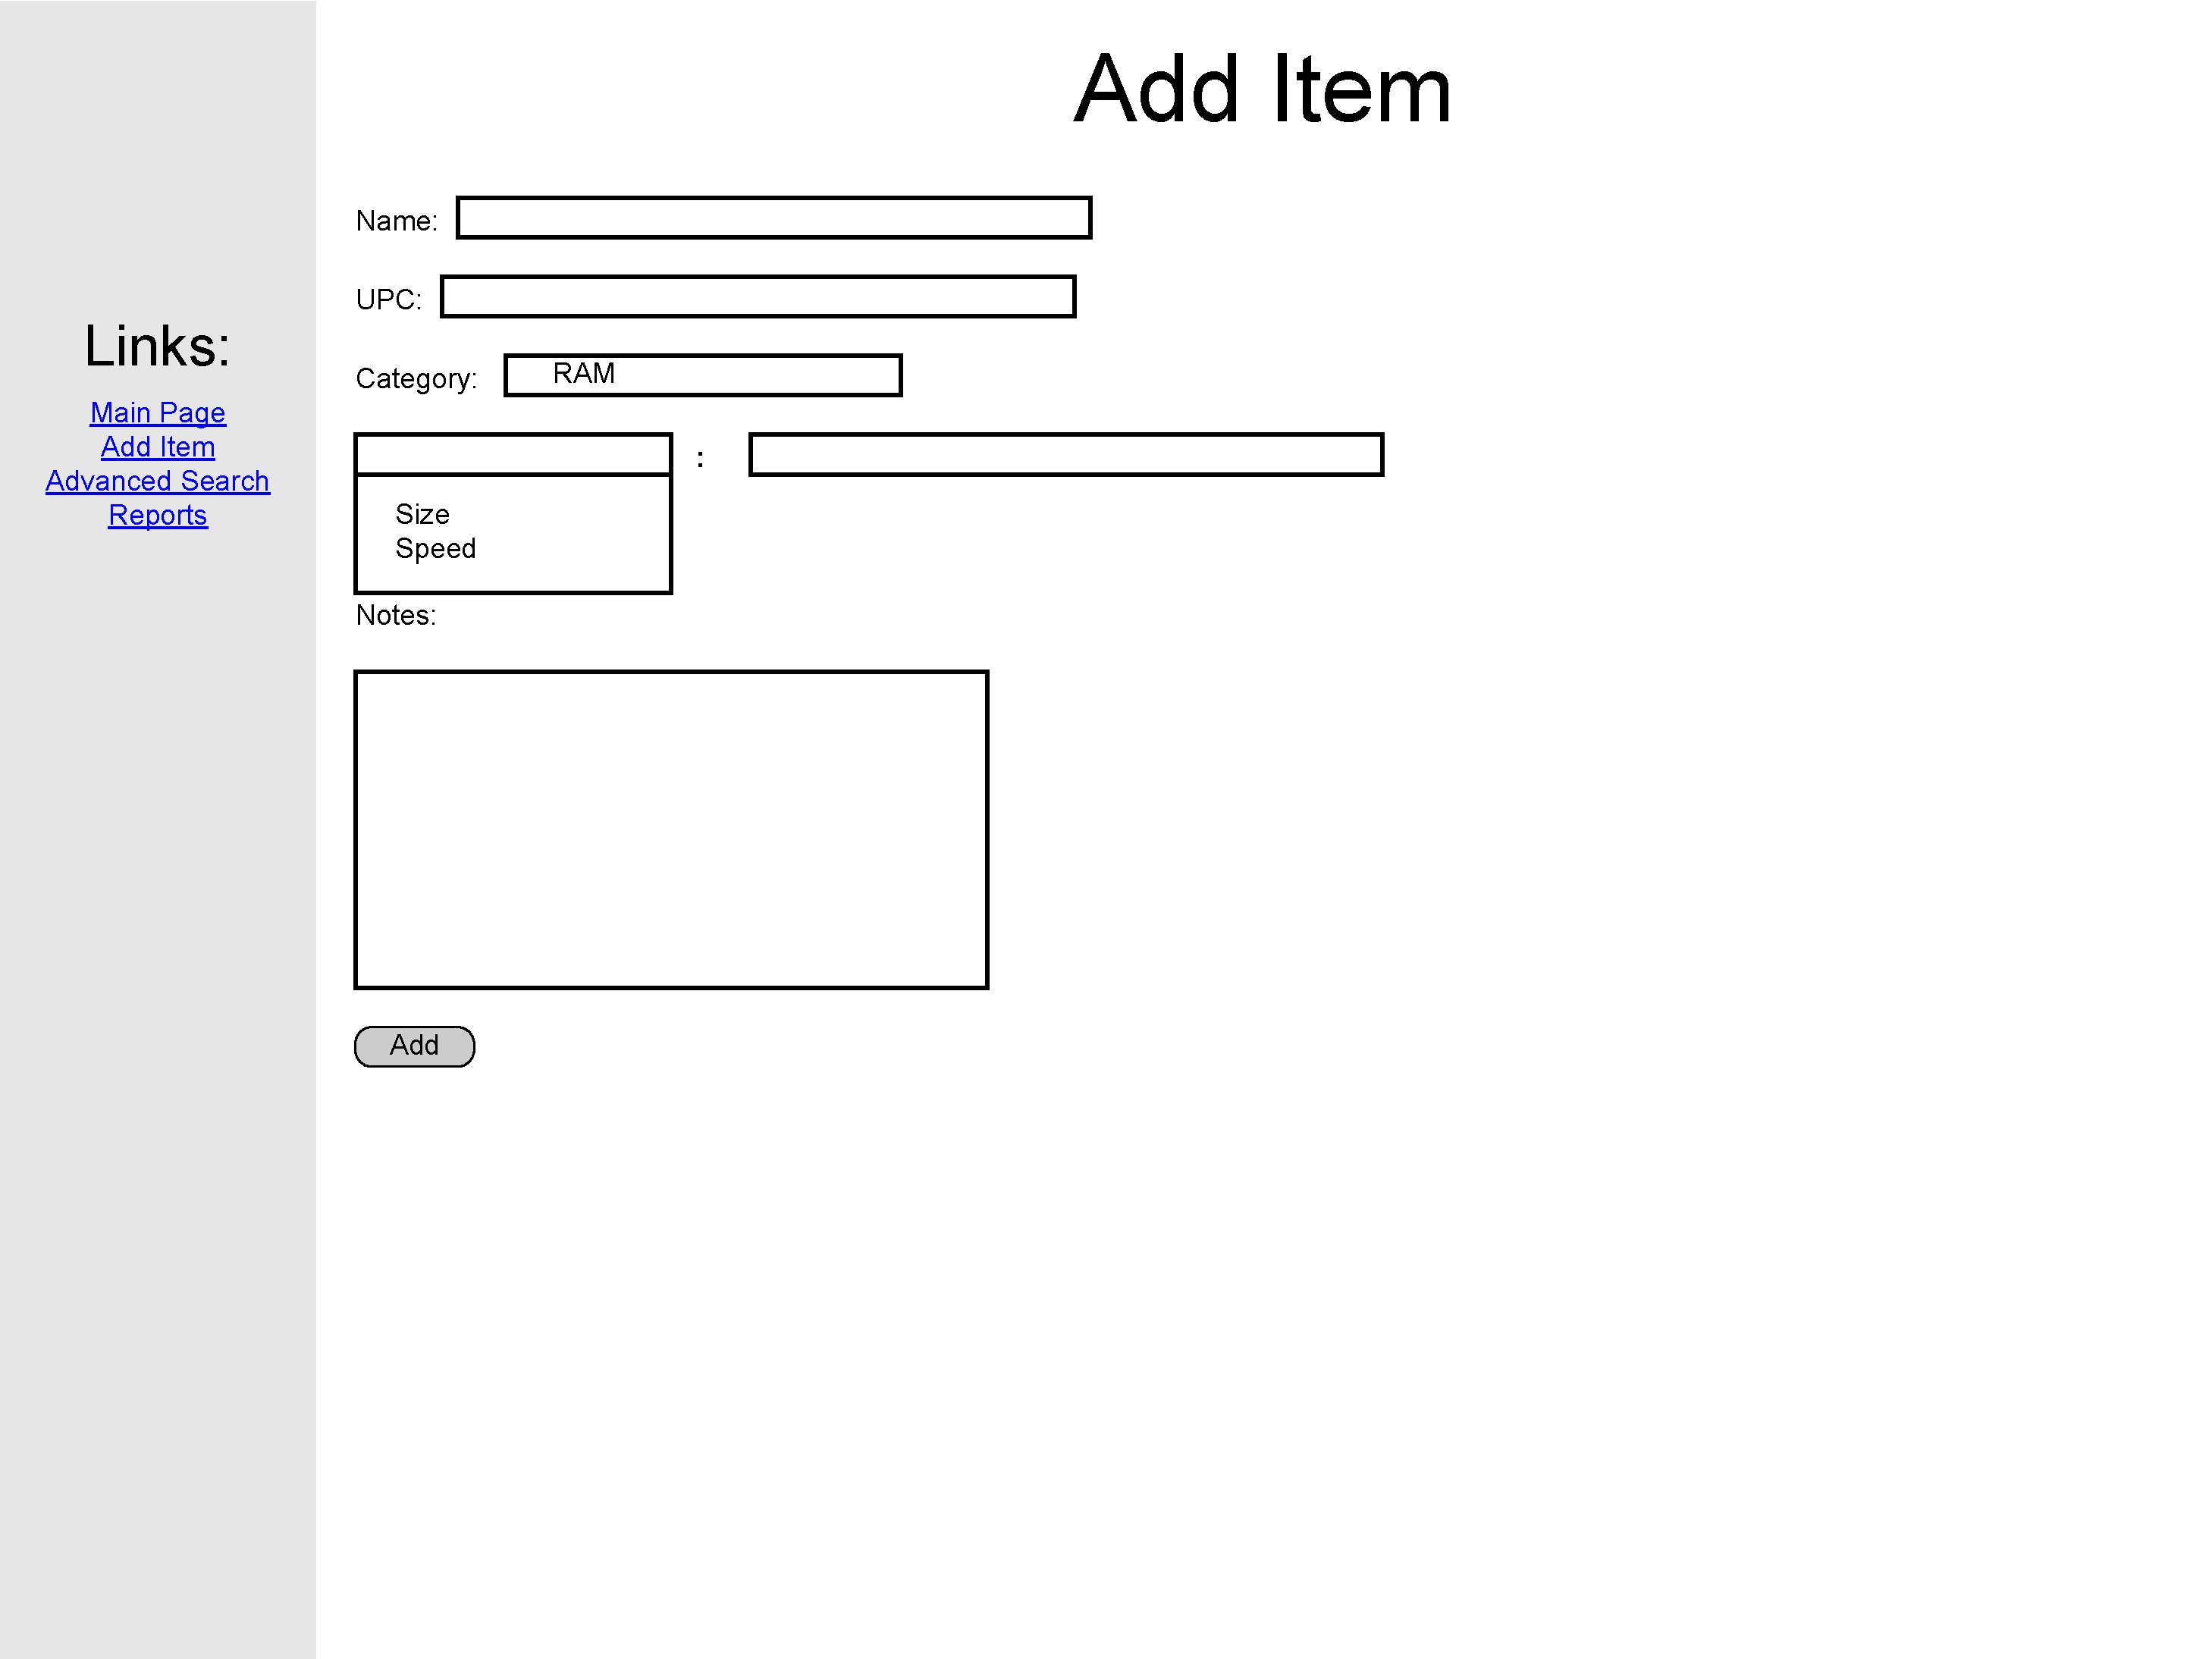
\includegraphics[keepaspectratio, width=4.5in]{addItemF0S2.pdf}  \\
The add item page with category selected and attribute autocomplete showing
\end{tabular}\\
~\\
~\\
\begin{tabular}{ p{4.5in} }
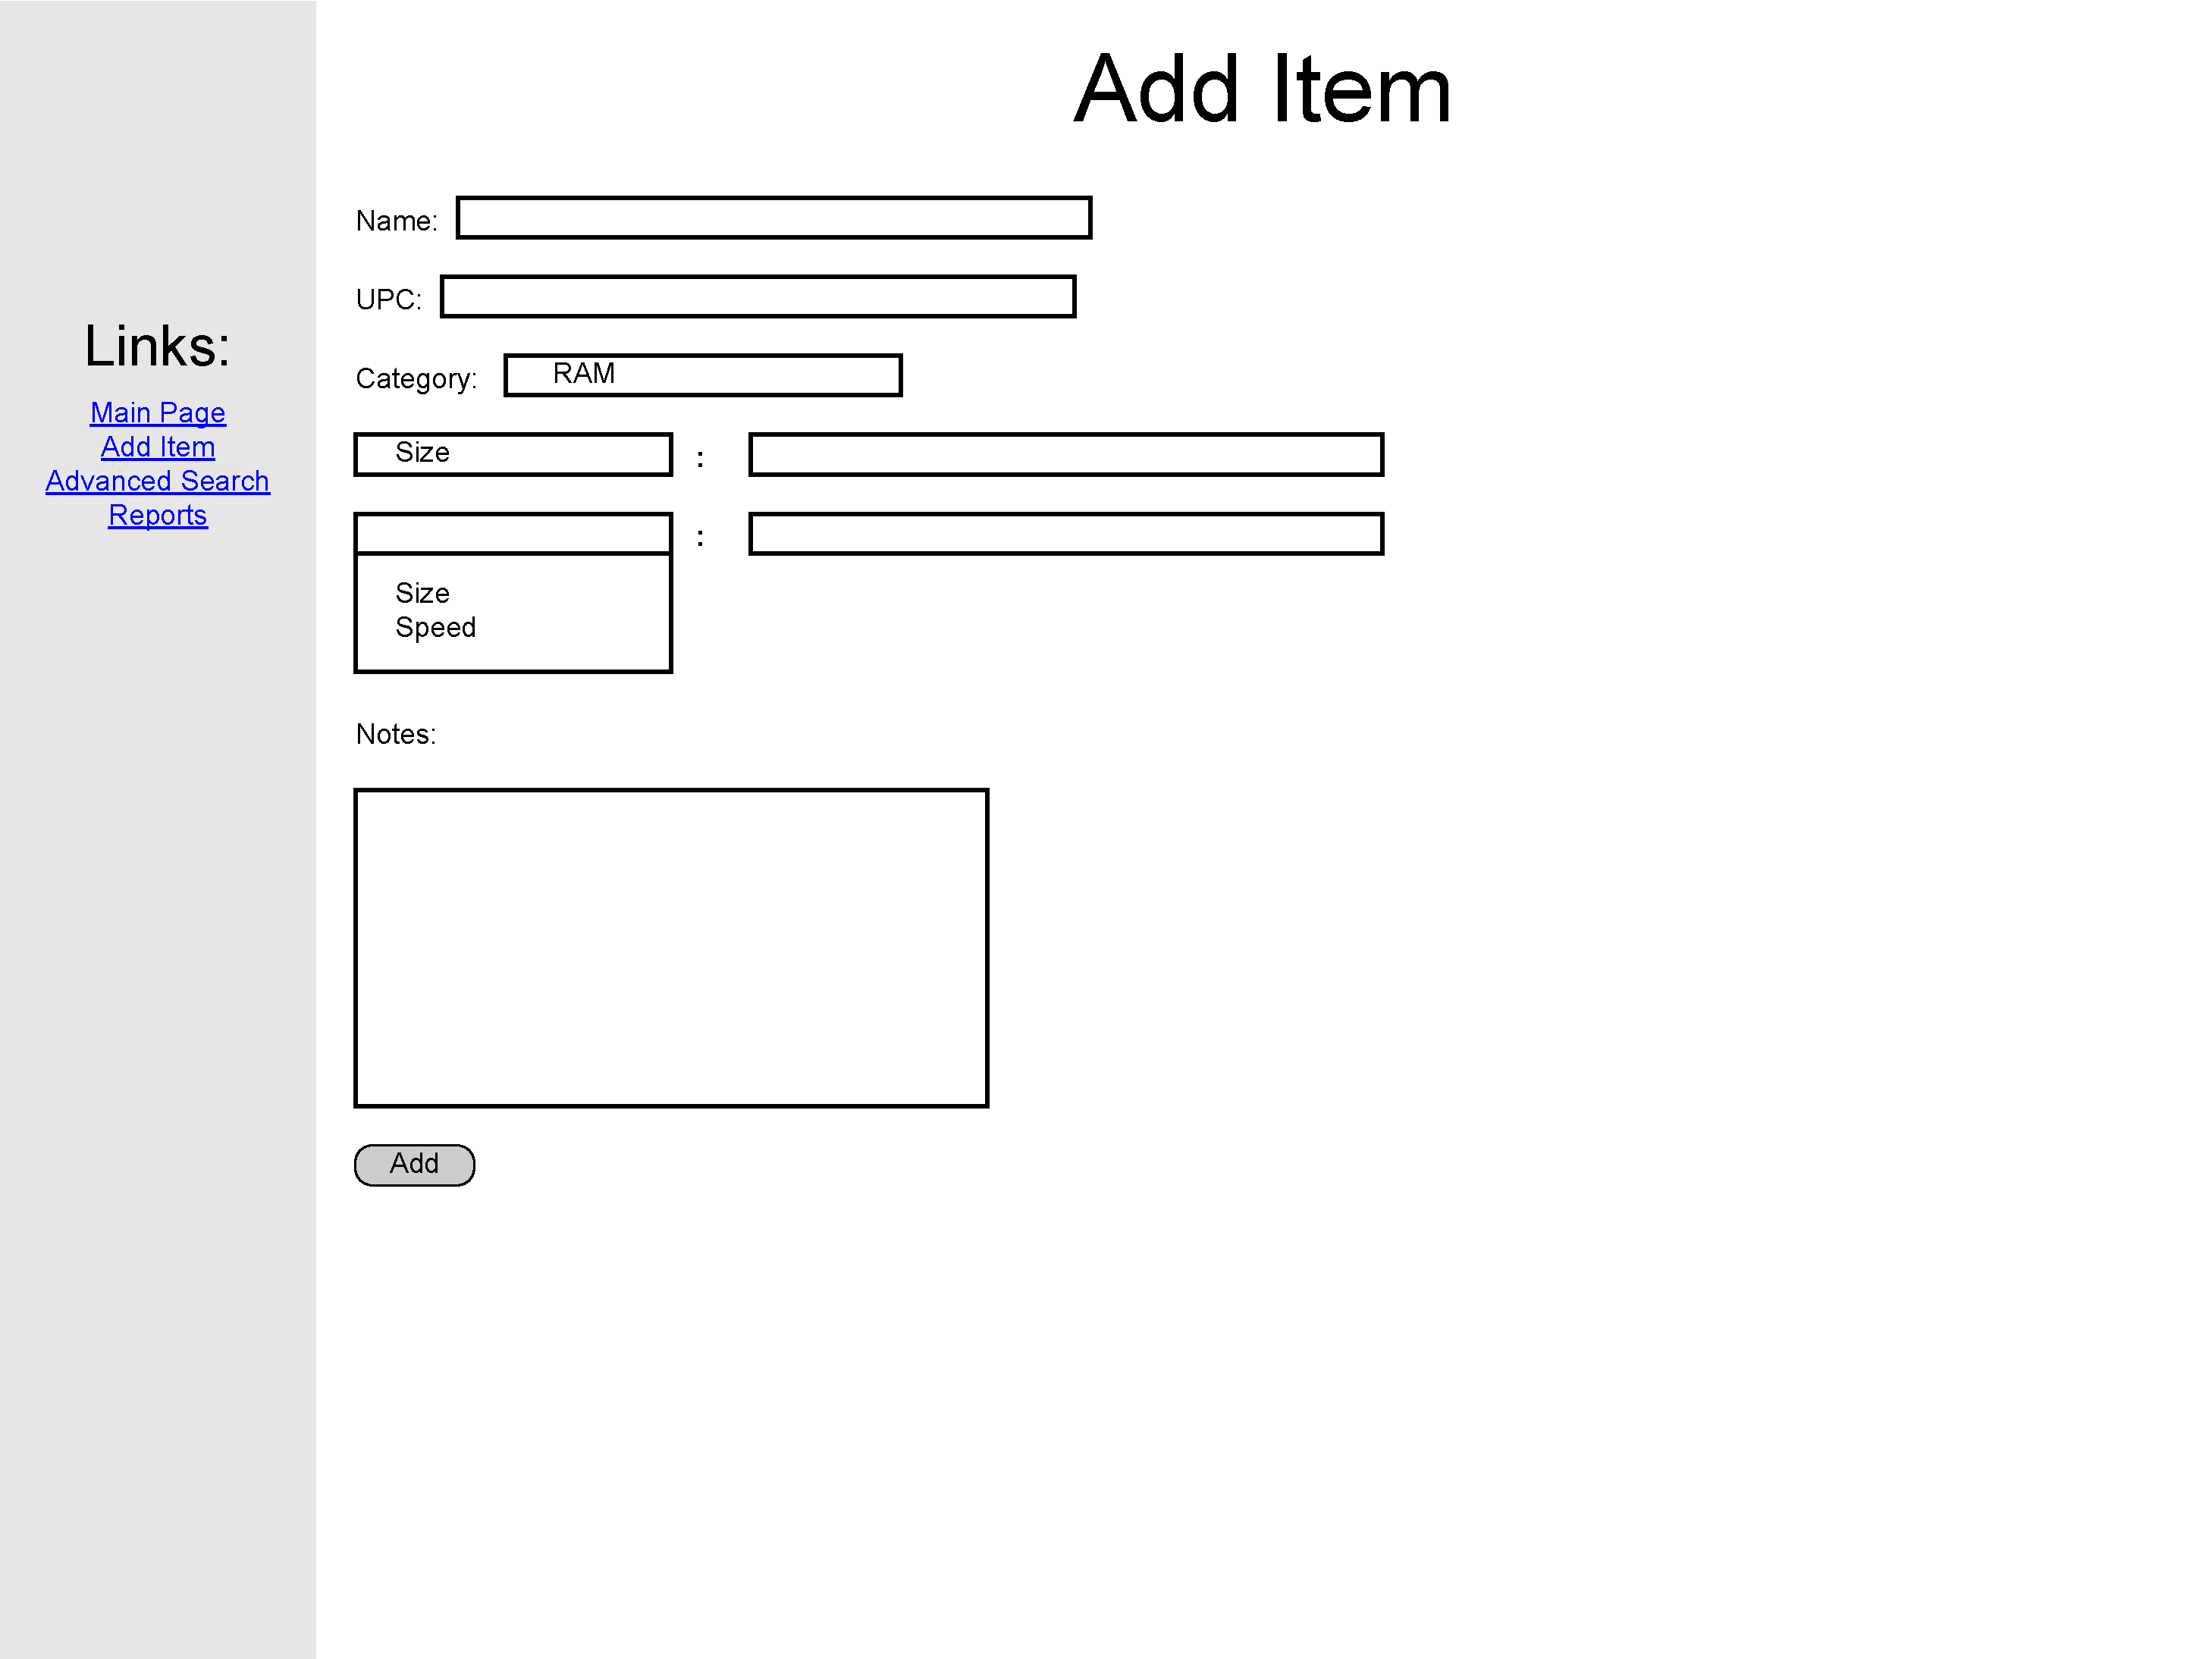
\includegraphics[keepaspectratio, width=4.5in]{addItemF0S3.pdf}\\
The add item page after one attribute key has been selected and another field added
\end{tabular}\\
~\\
~\\
\begin{tabular}{ p{4.5in} }
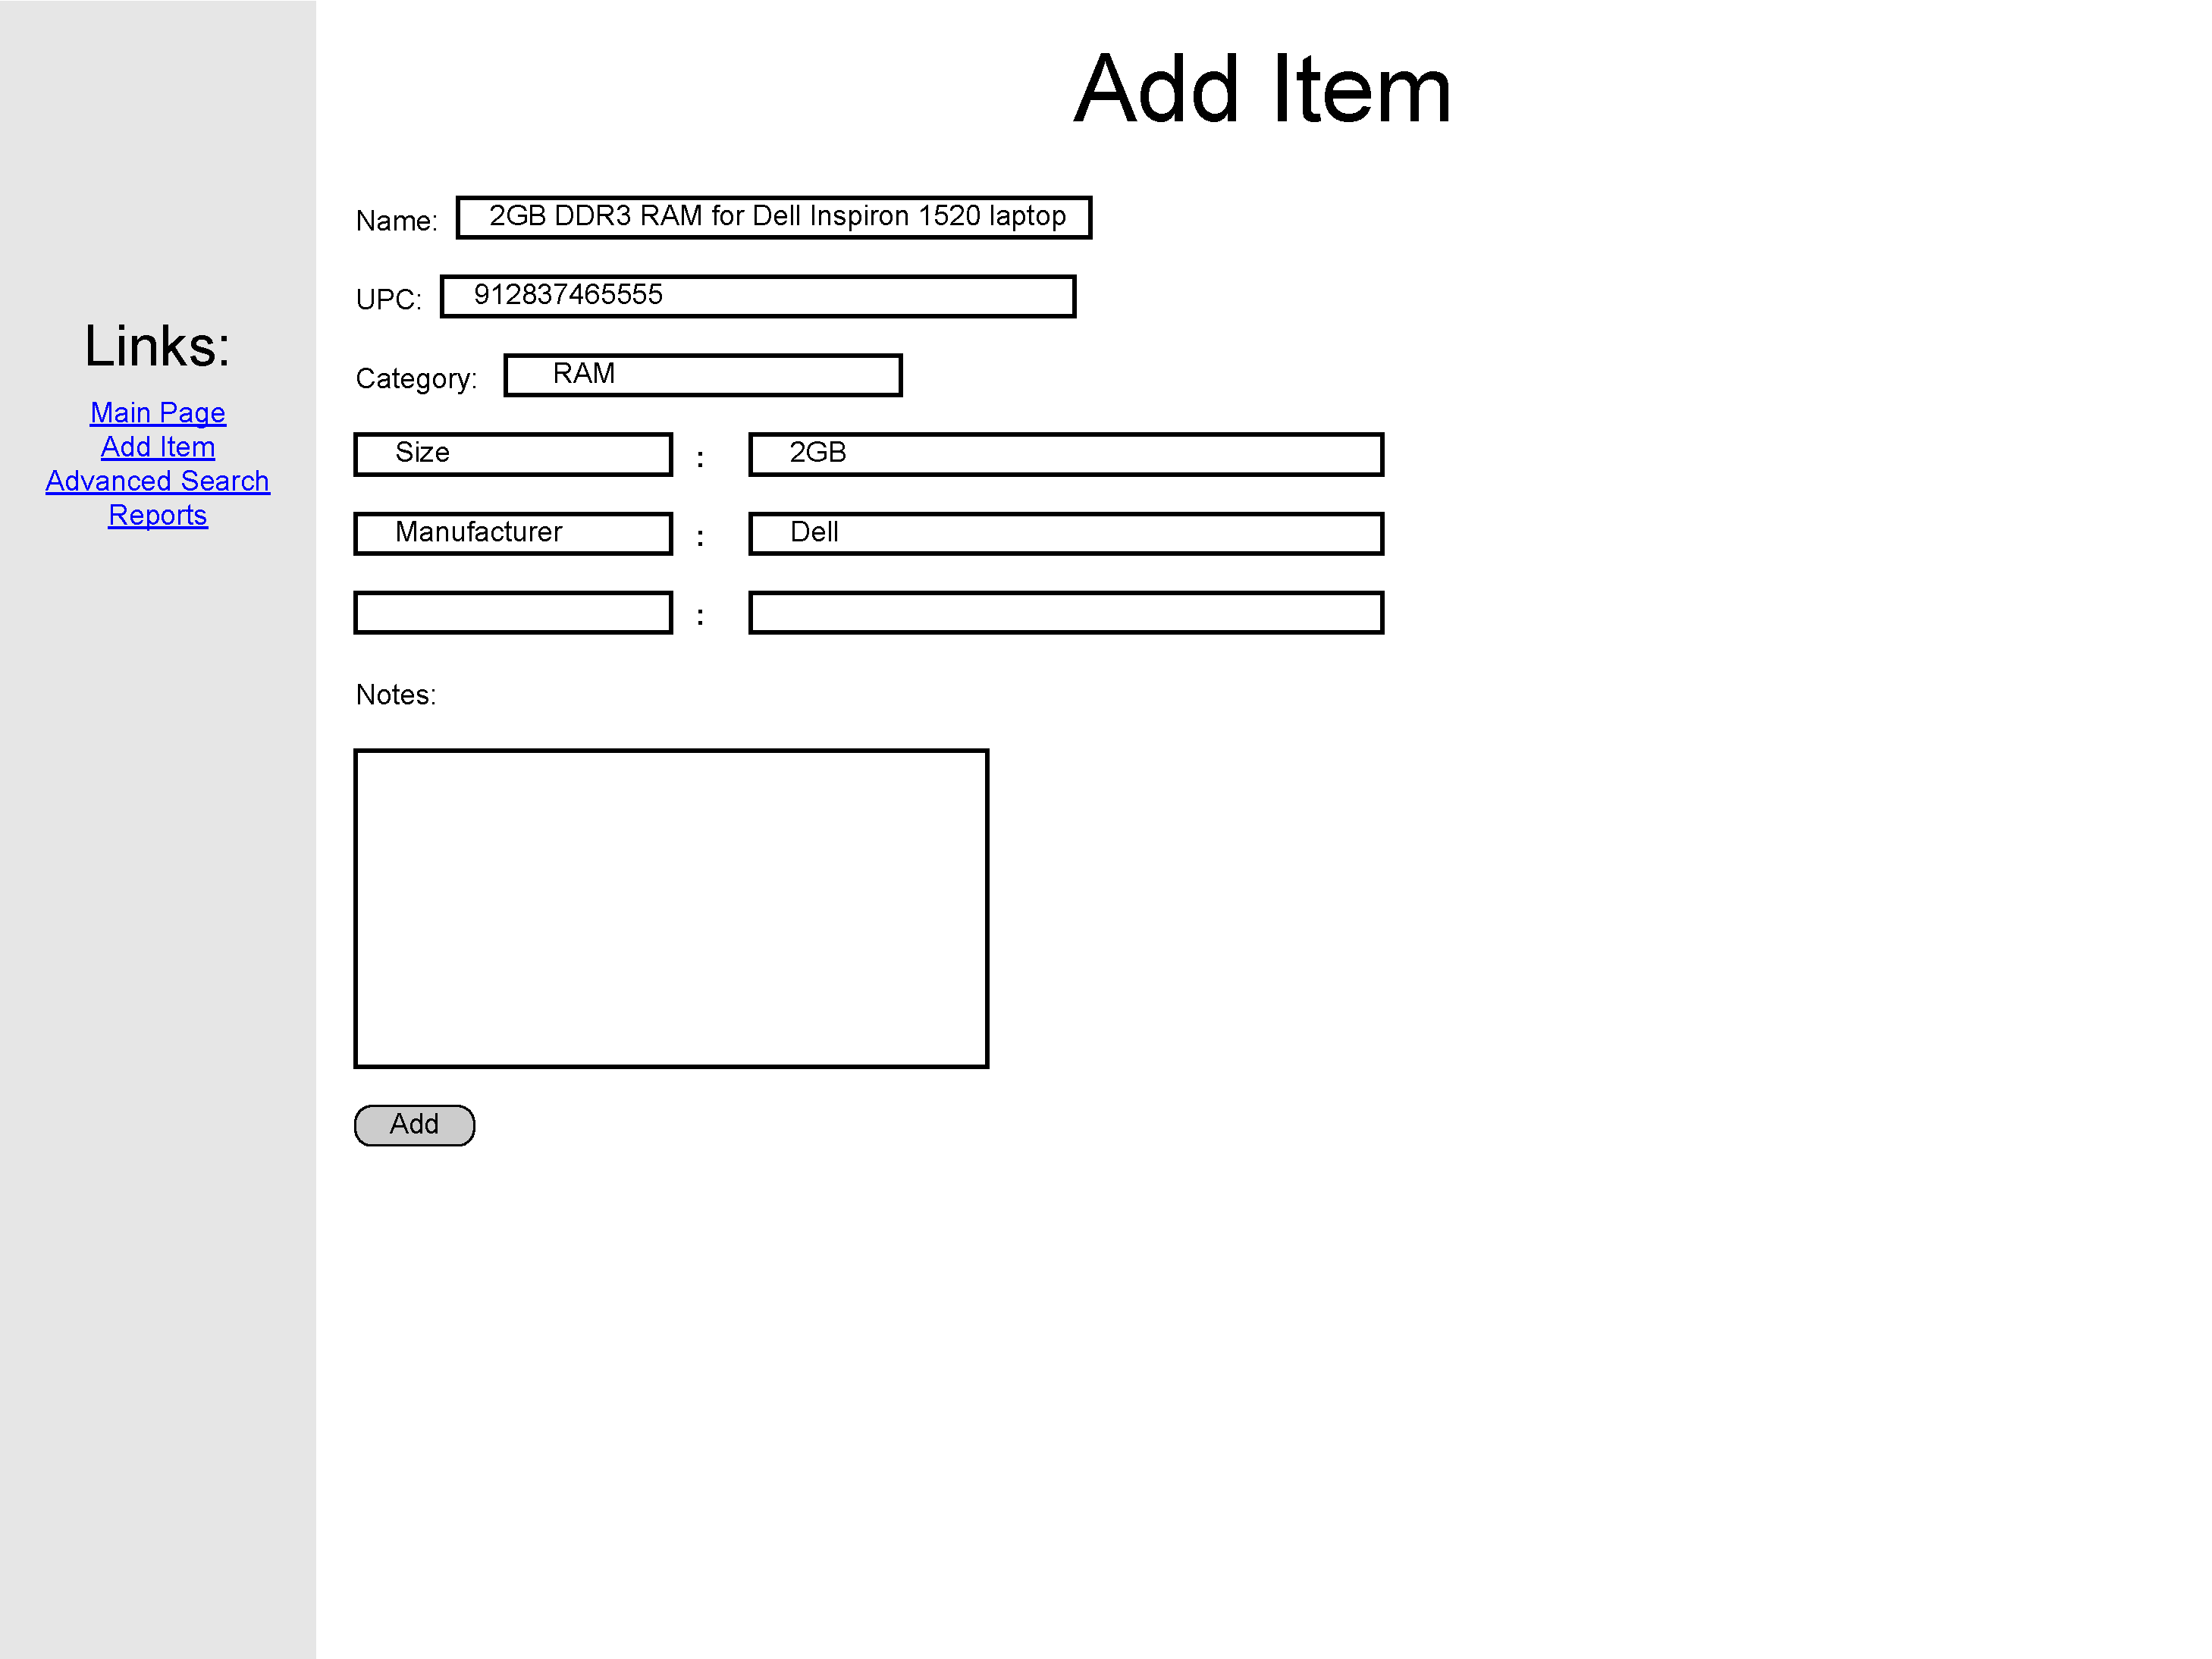
\includegraphics[keepaspectratio, width=4.5in]{addItemF0S5.pdf}\\
The add item page with data filled in, showing that arbitrary attribute names can be used.  It is also possible to use arbitrary categories.
\end{tabular}\\
~\\
~\\
\begin{tabular}{ p{4.5in} }
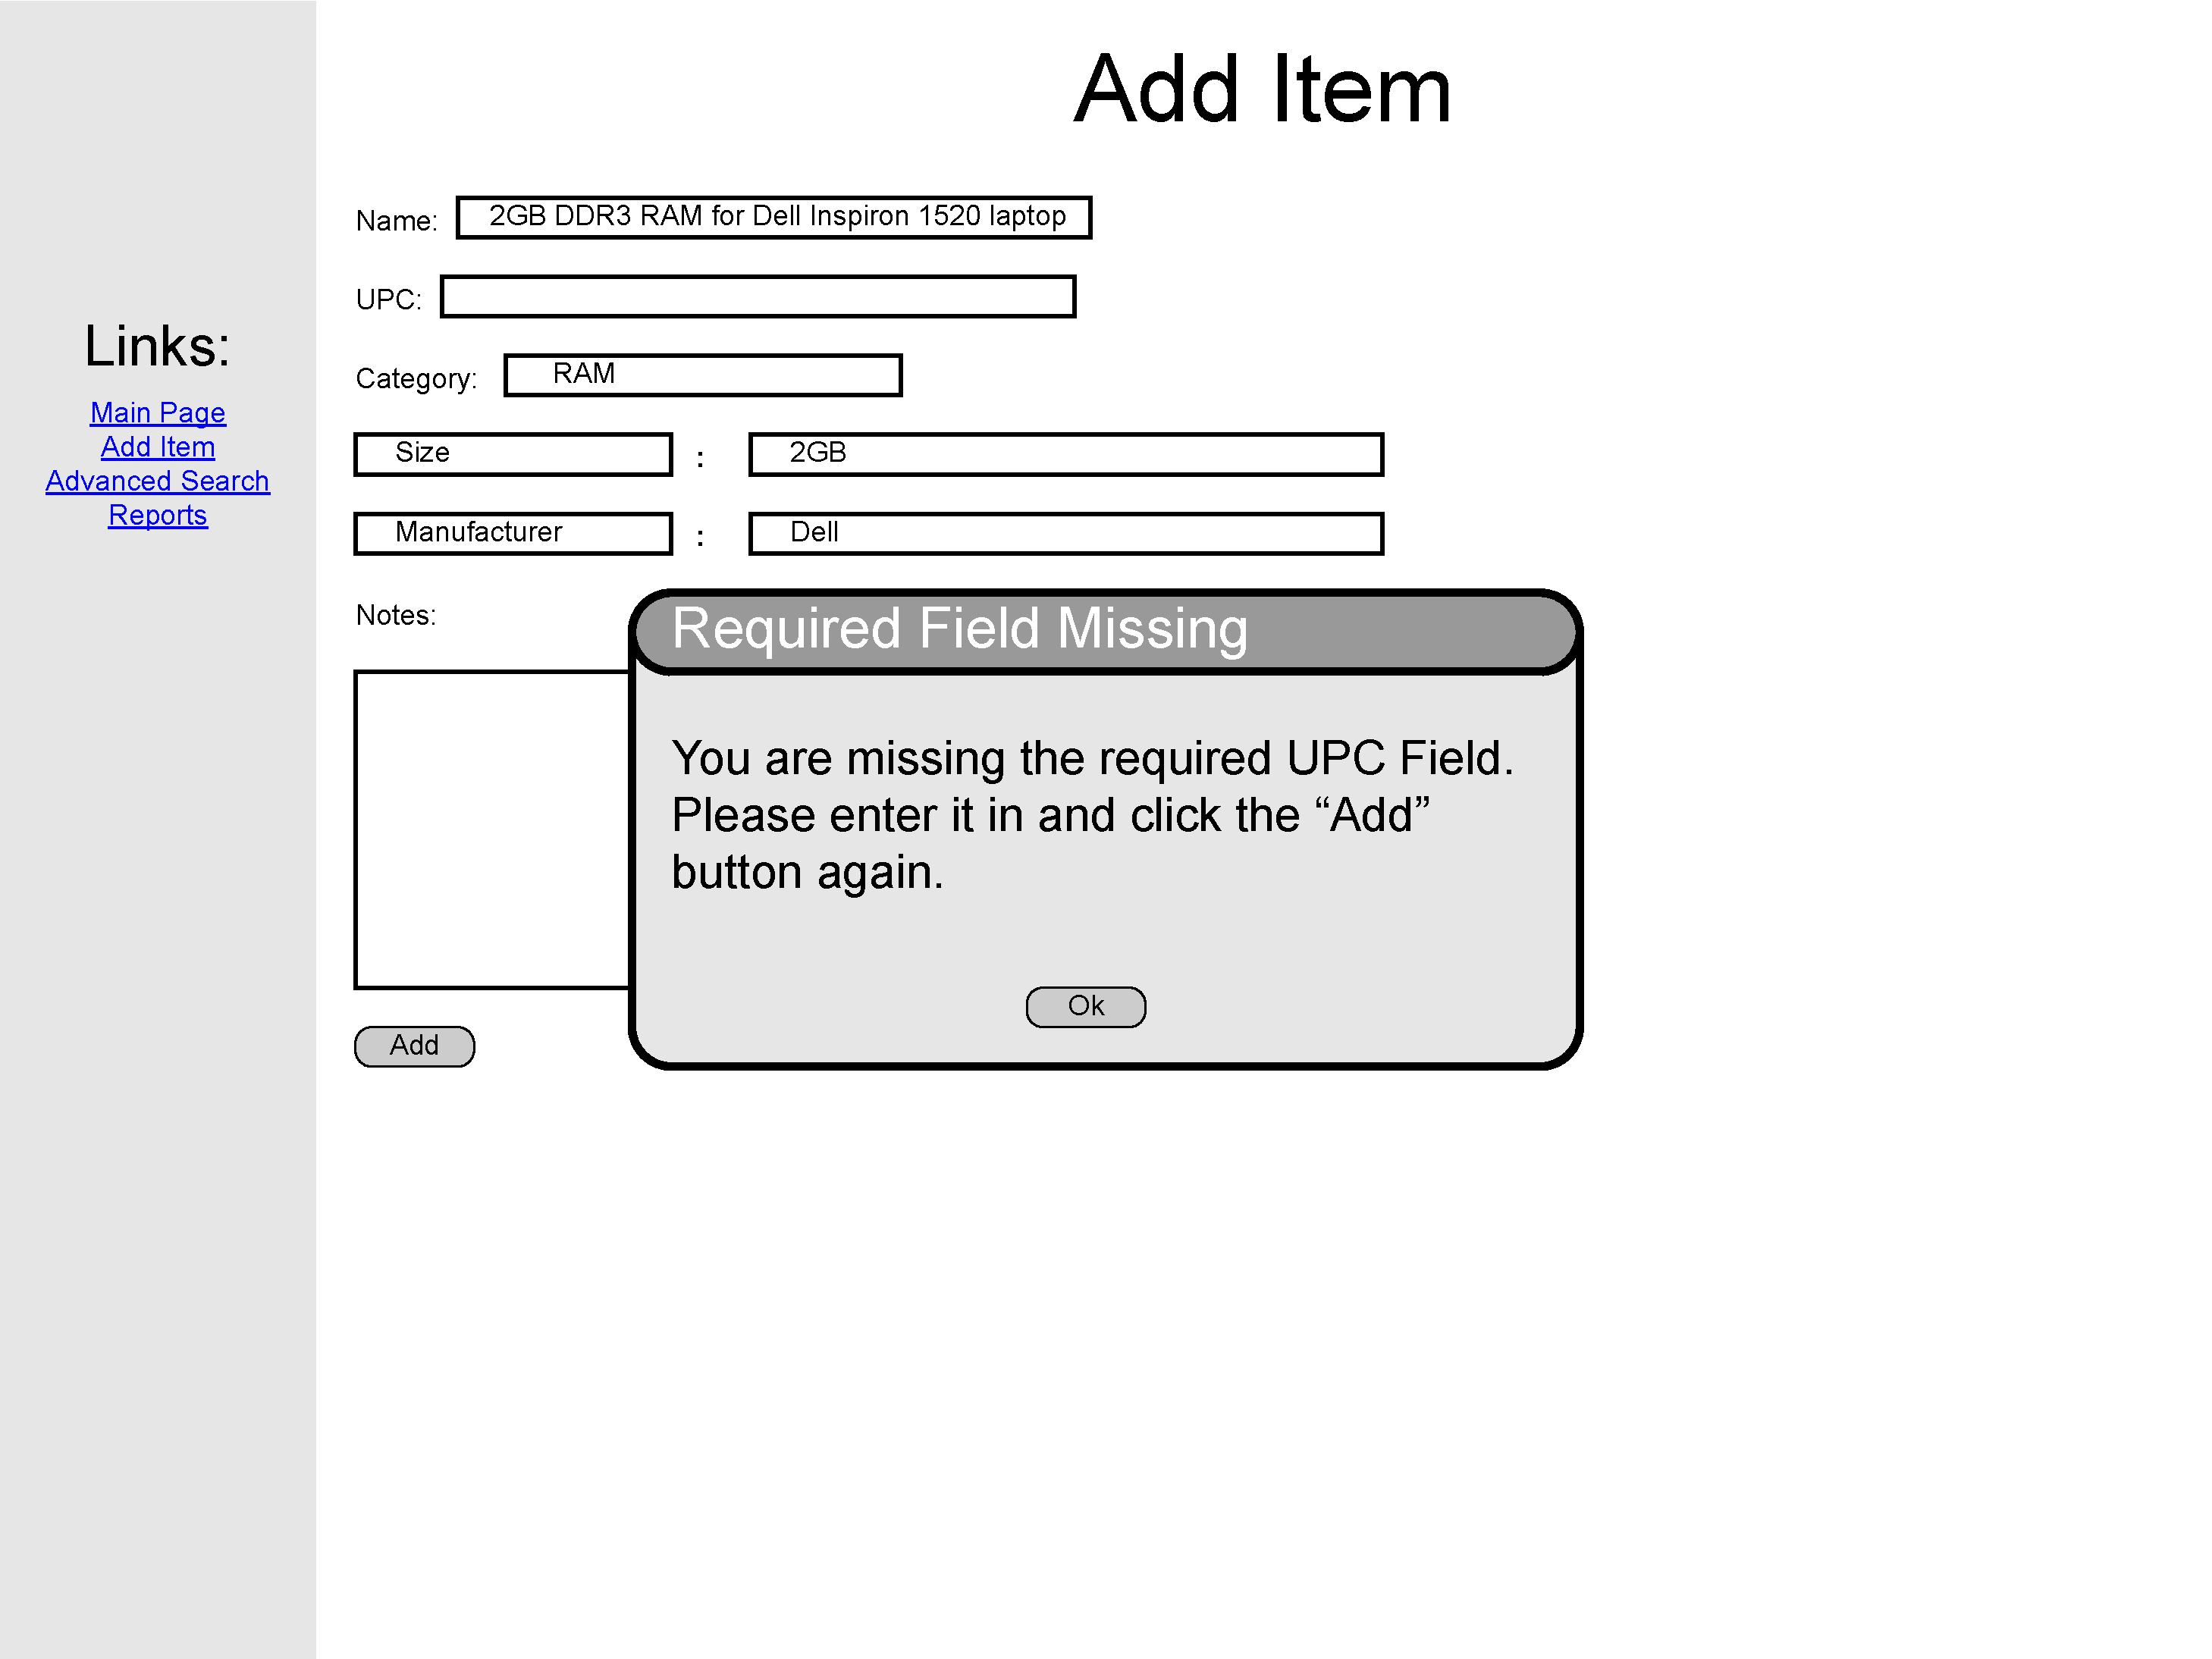
\includegraphics[keepaspectratio, width=4.5in]{addItemF1S5.pdf} \\
Popup message informing the user that the required UPC field is missing
\end{tabular}\\
~\\
~\\
\begin{tabular}{ p{4.5in} }
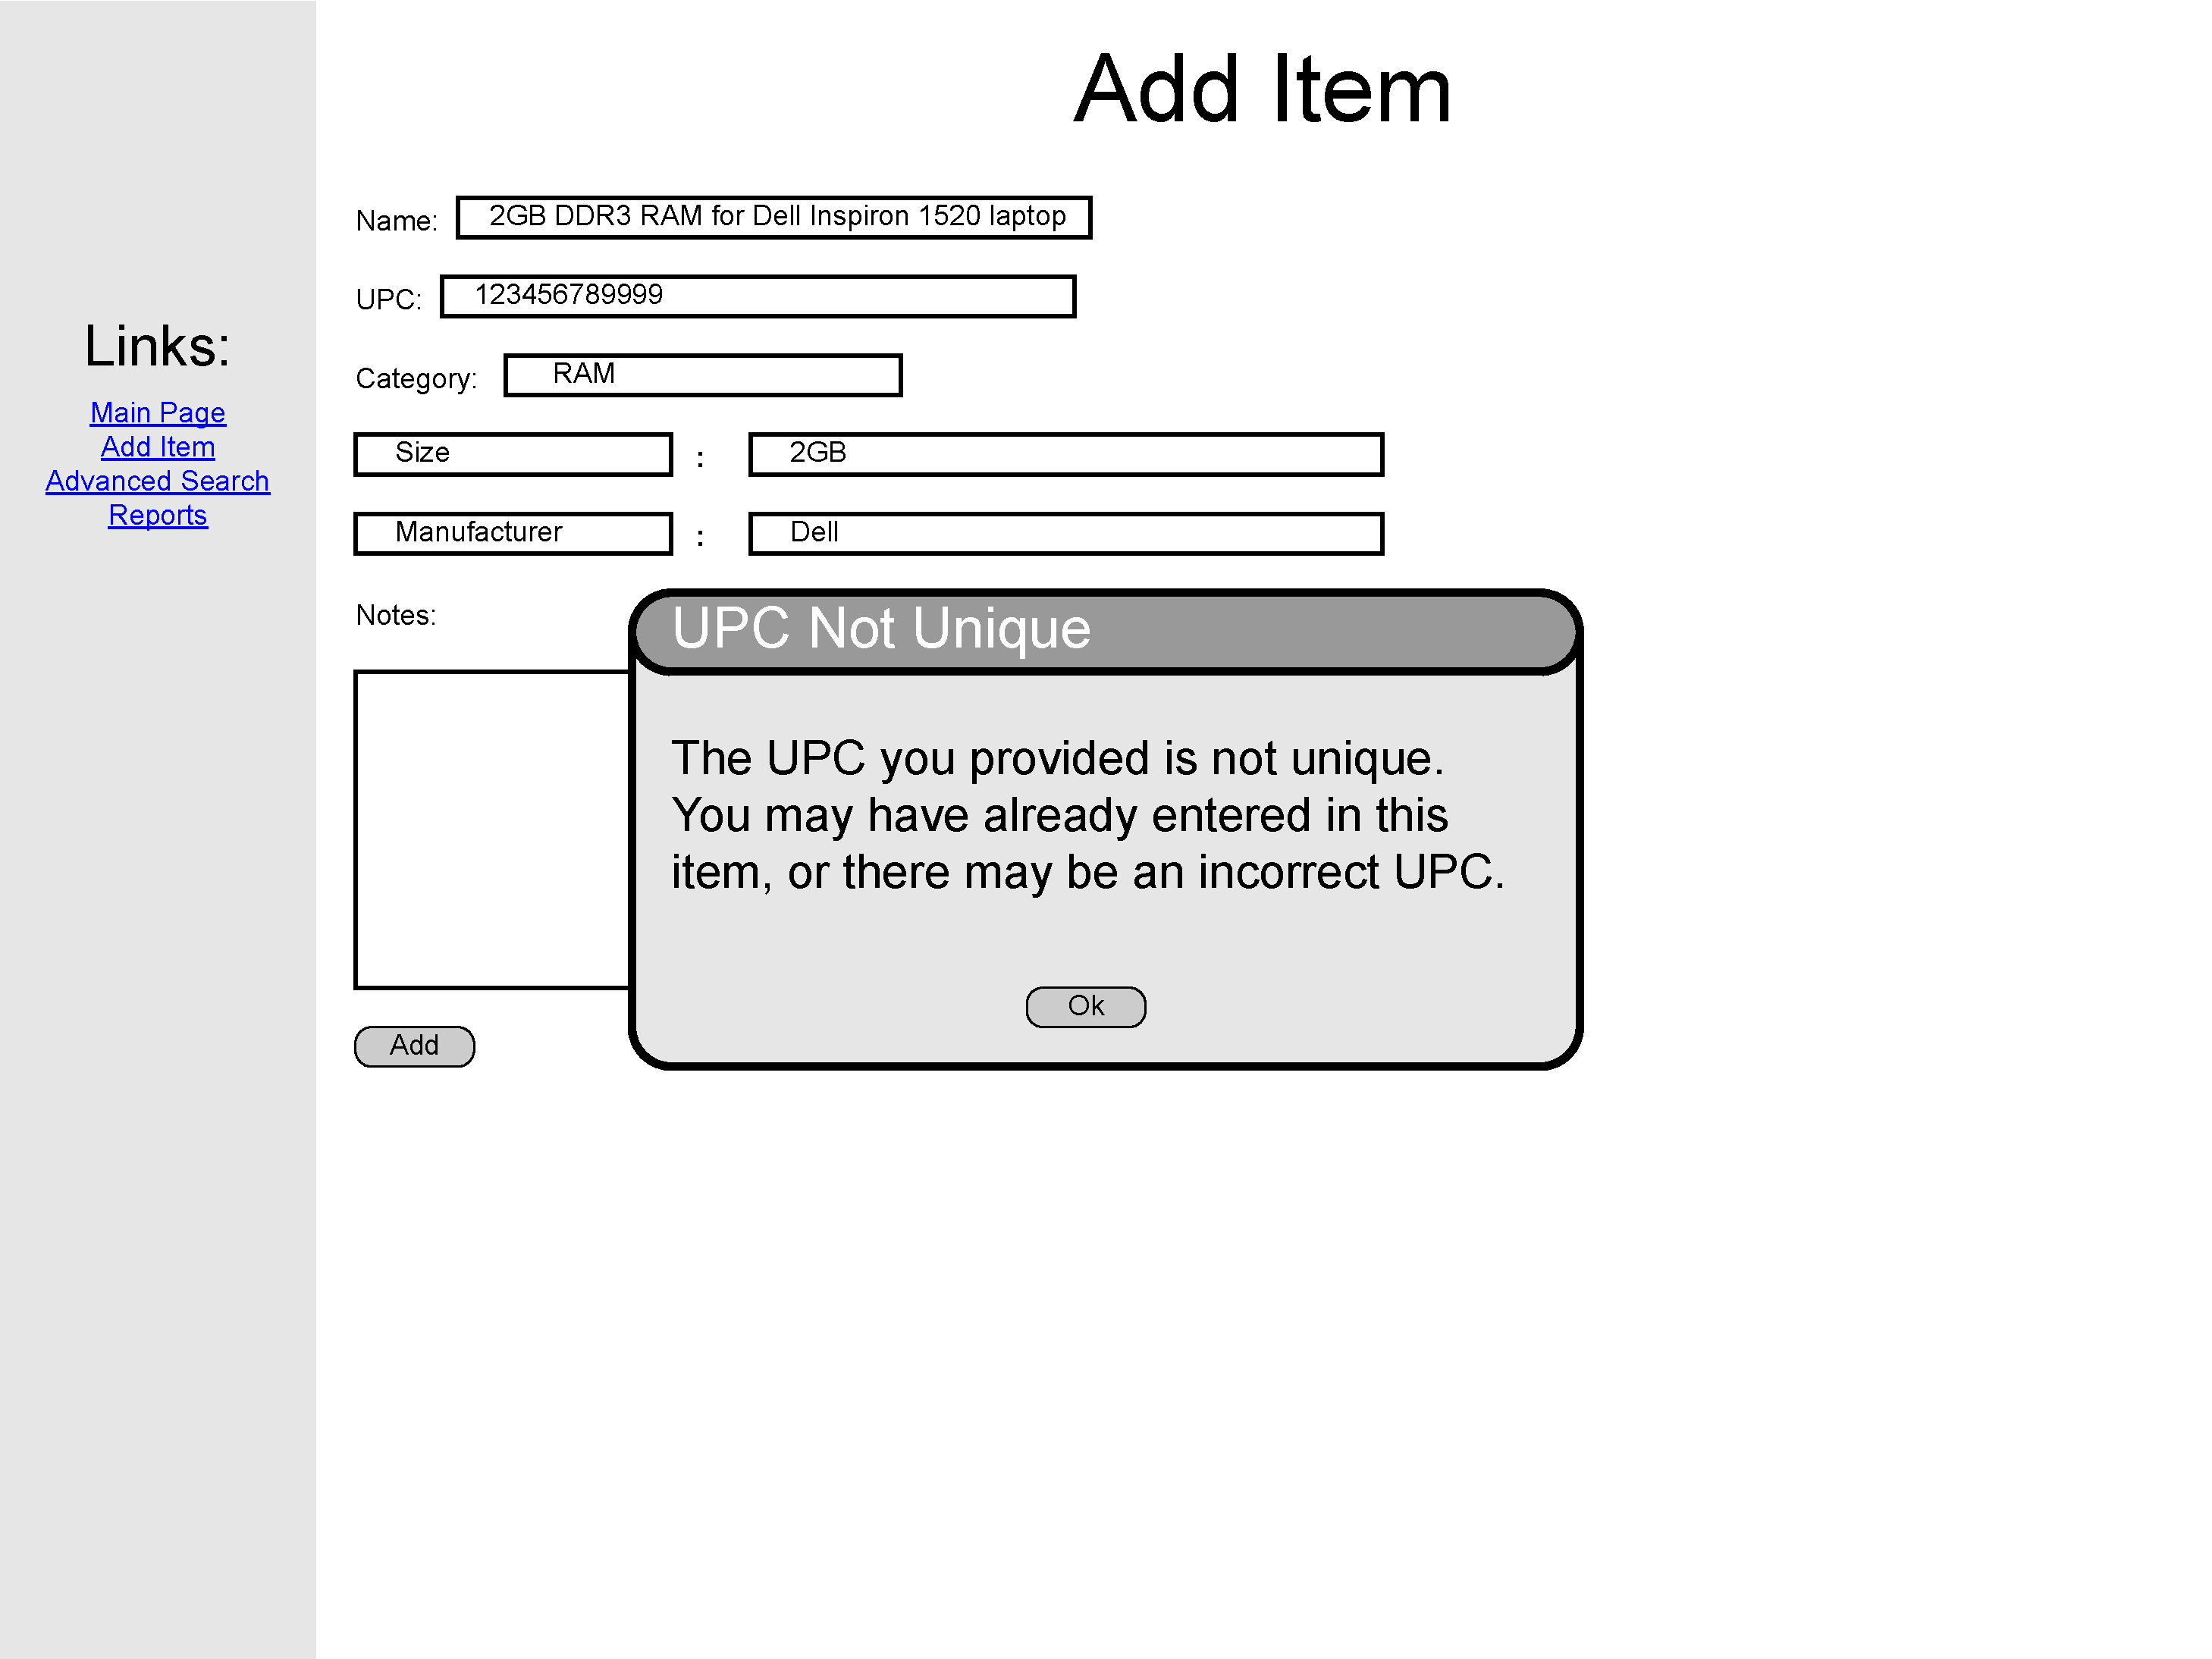
\includegraphics[keepaspectratio, width=4.5in]{addItemF2S5.pdf} \\
Popup message informing the user that the UPC entered has been previously entered
\end{tabular}\\
~\\
~\\
\begin{tabular}{ p{4.5in} }
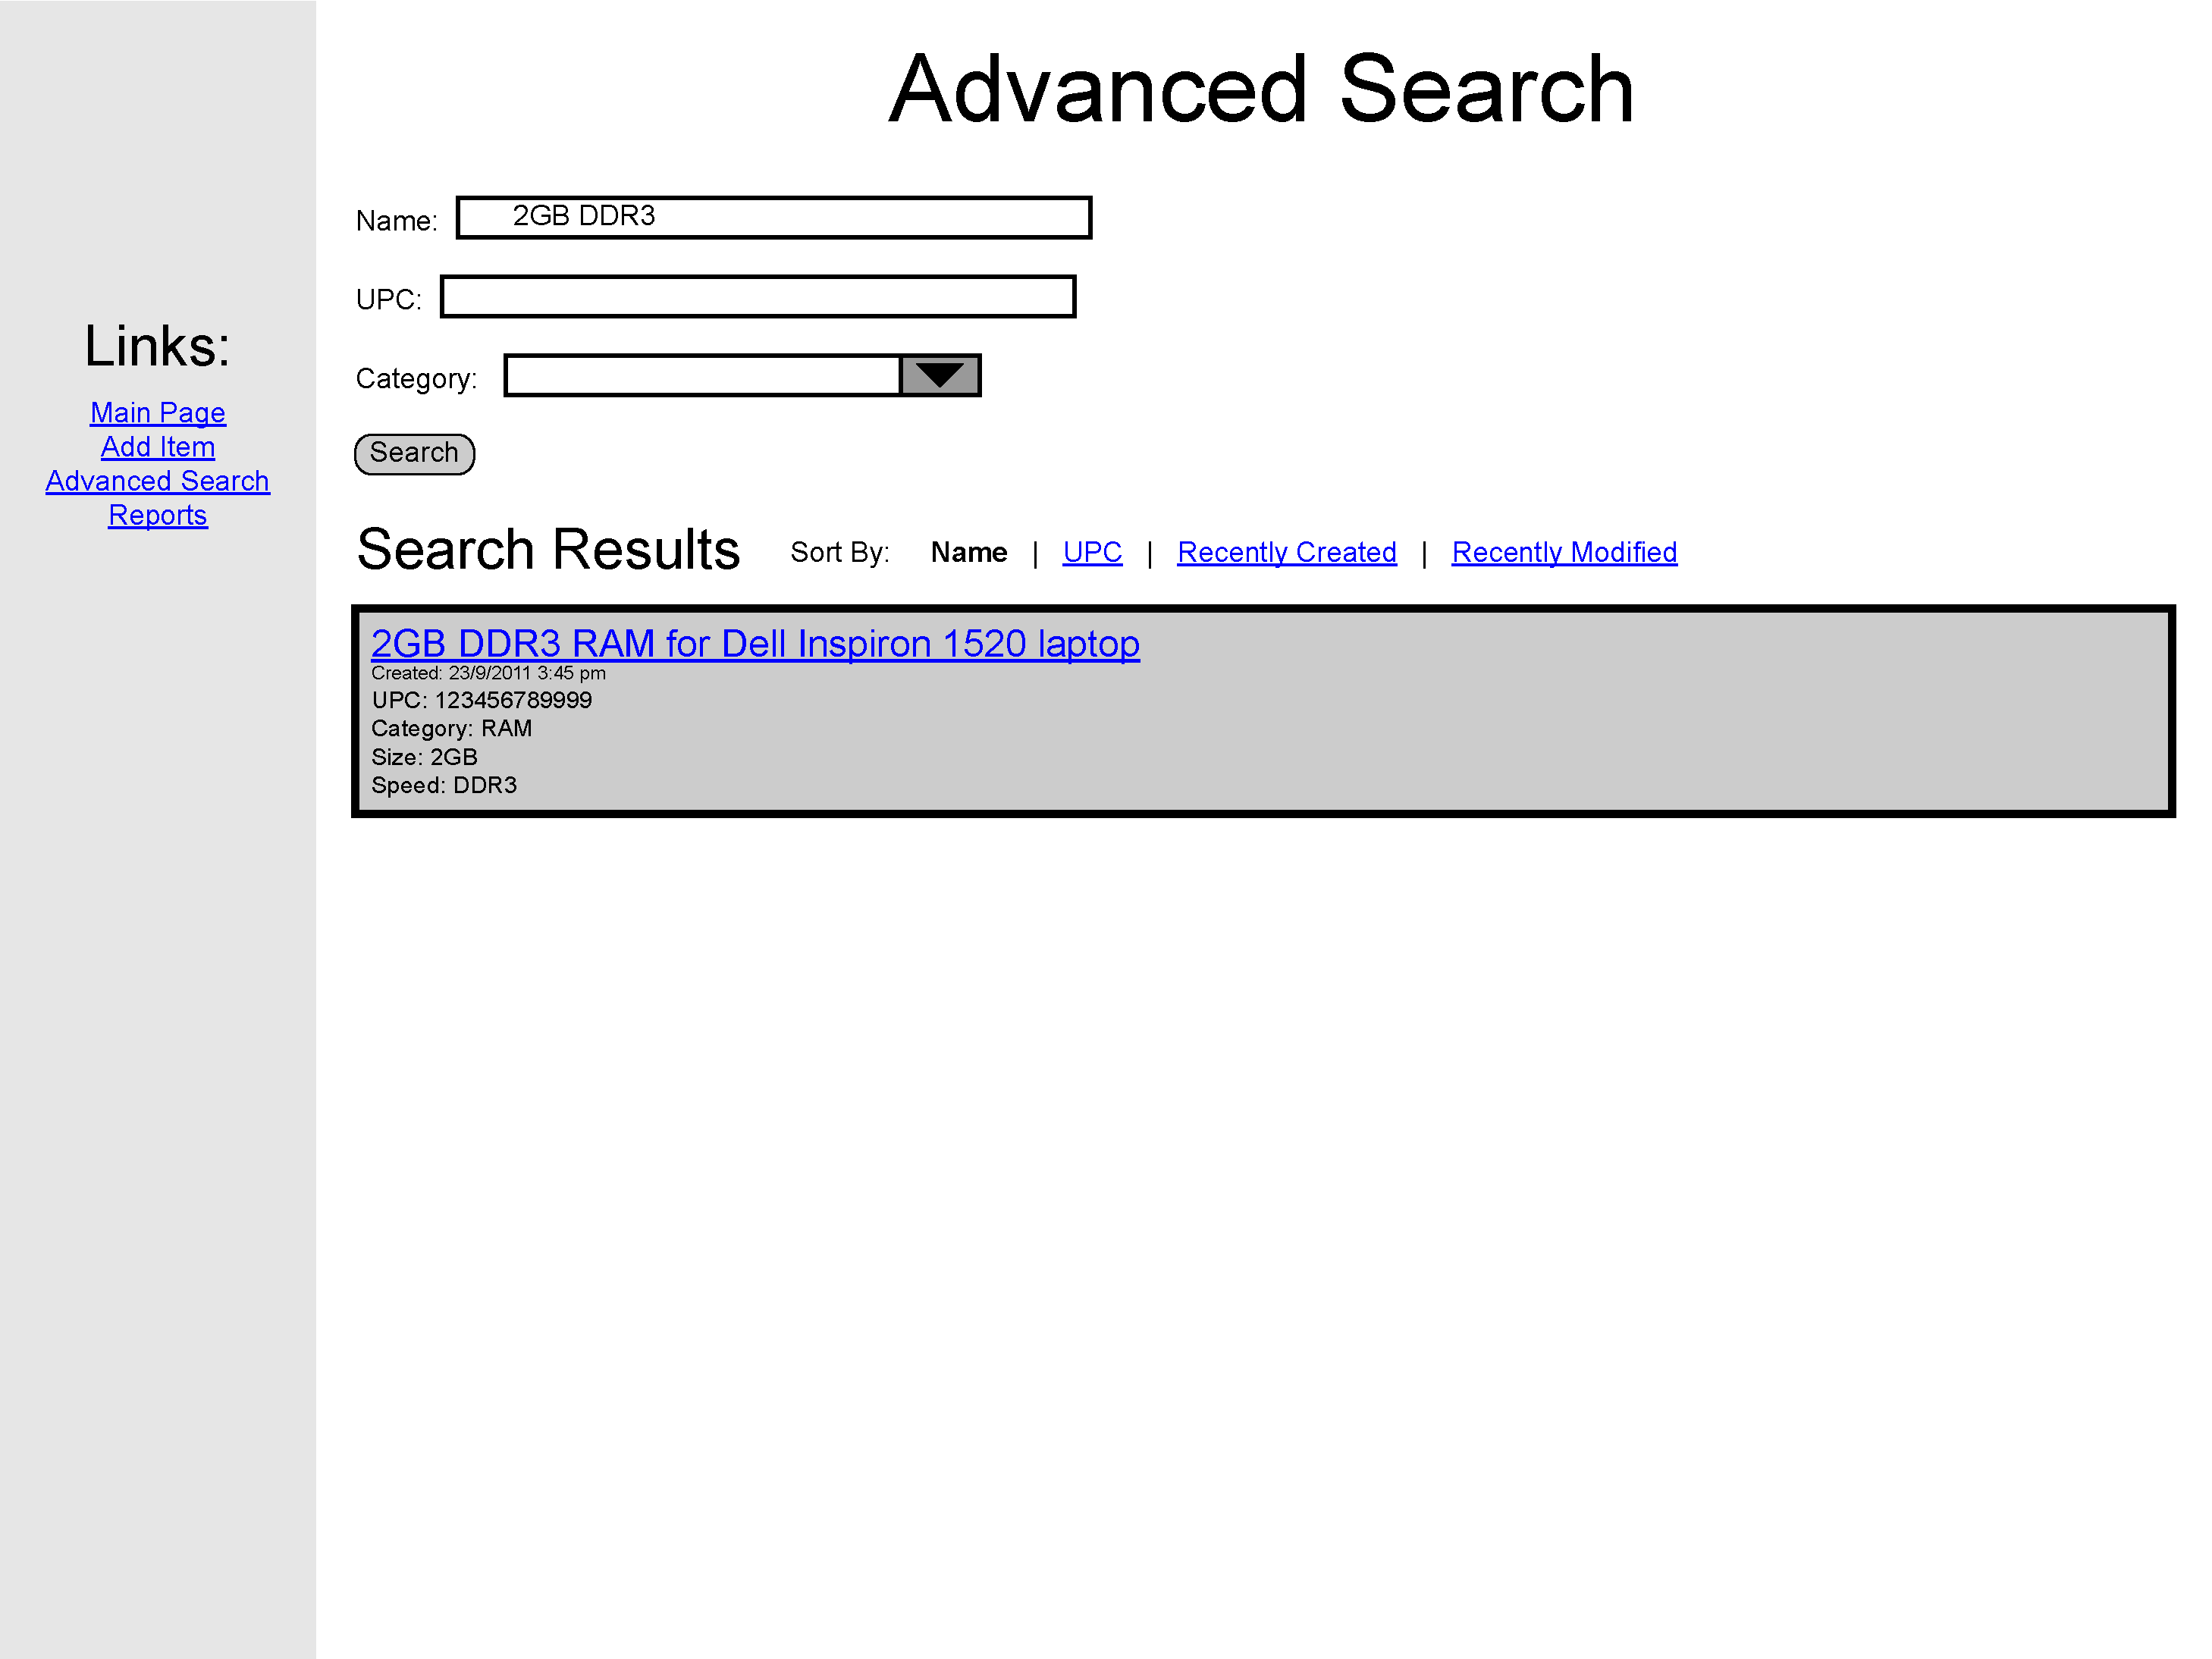
\includegraphics[keepaspectratio, width=4.5in]{basicSearchF0S1.pdf} \\
The results of the basic search, showing all of the results on one page
\end{tabular}\\
~\\
~\\
\begin{tabular}{ p{4.5in} }
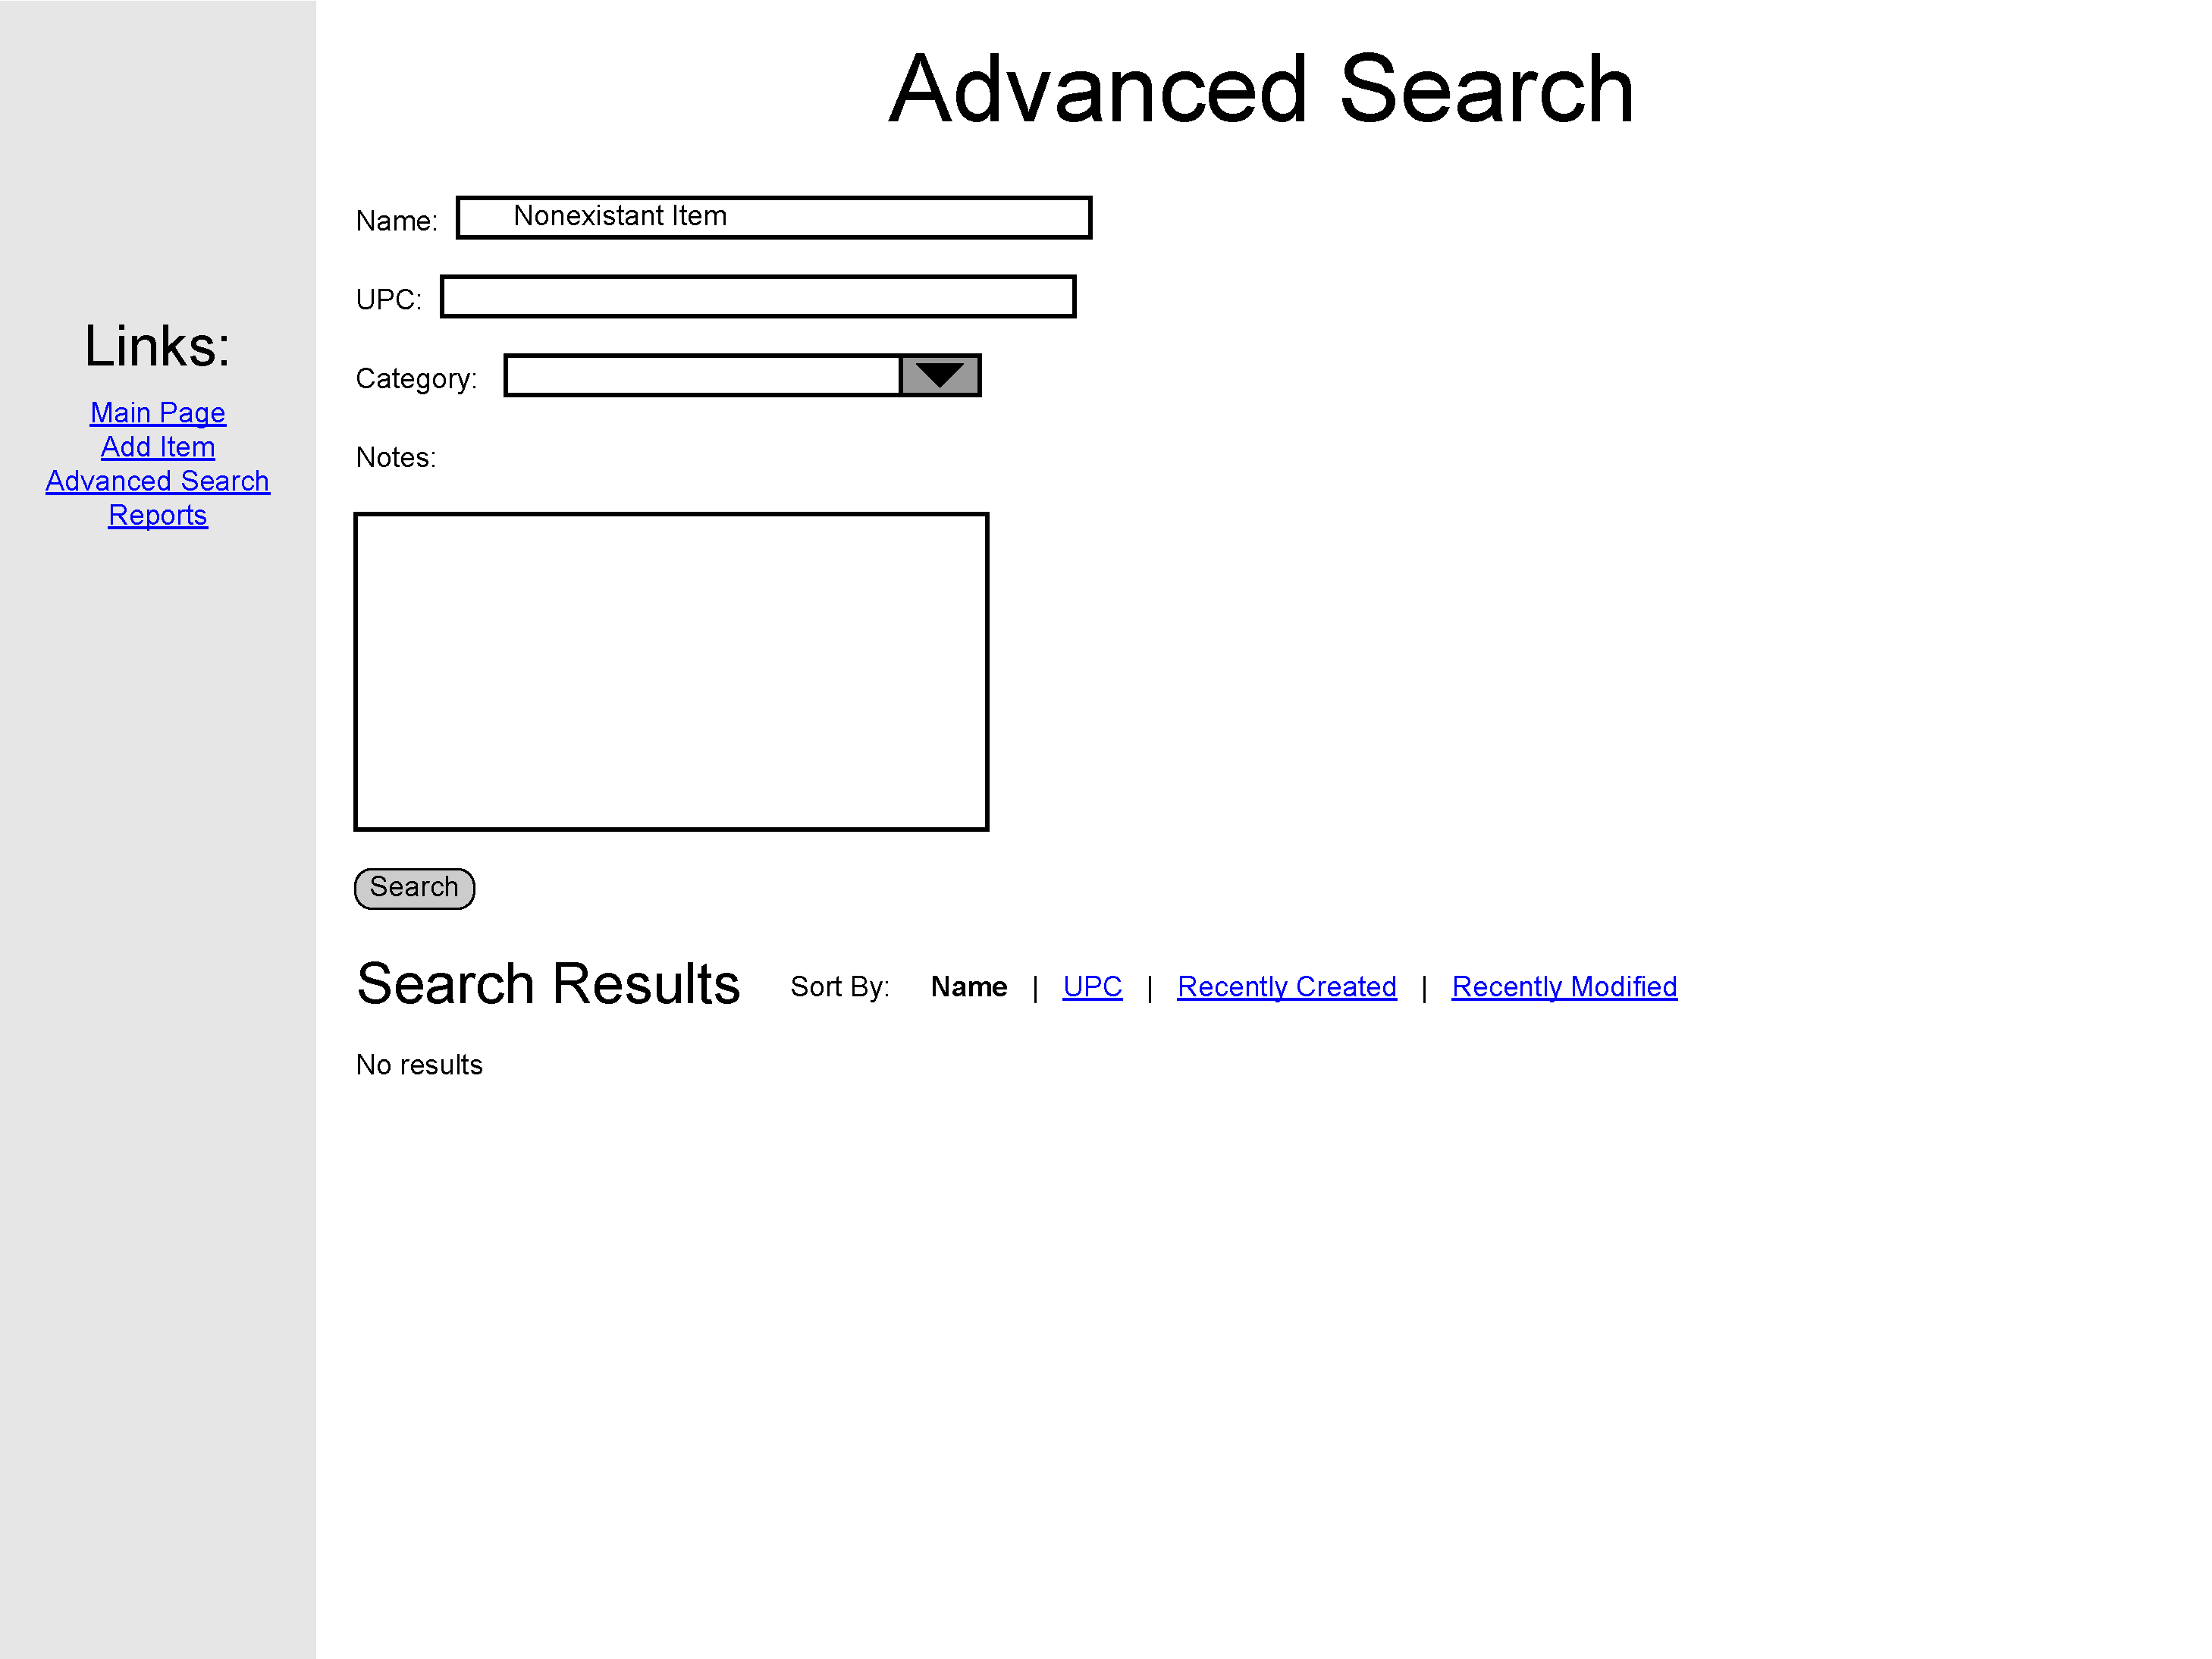
\includegraphics[keepaspectratio, width=4.5in]{basicSearchF2S1.pdf} \\
The results of the basic search when there are no matching entries
\end{tabular}\\
~\\
~\\
\begin{tabular}{ p{4.5in} }
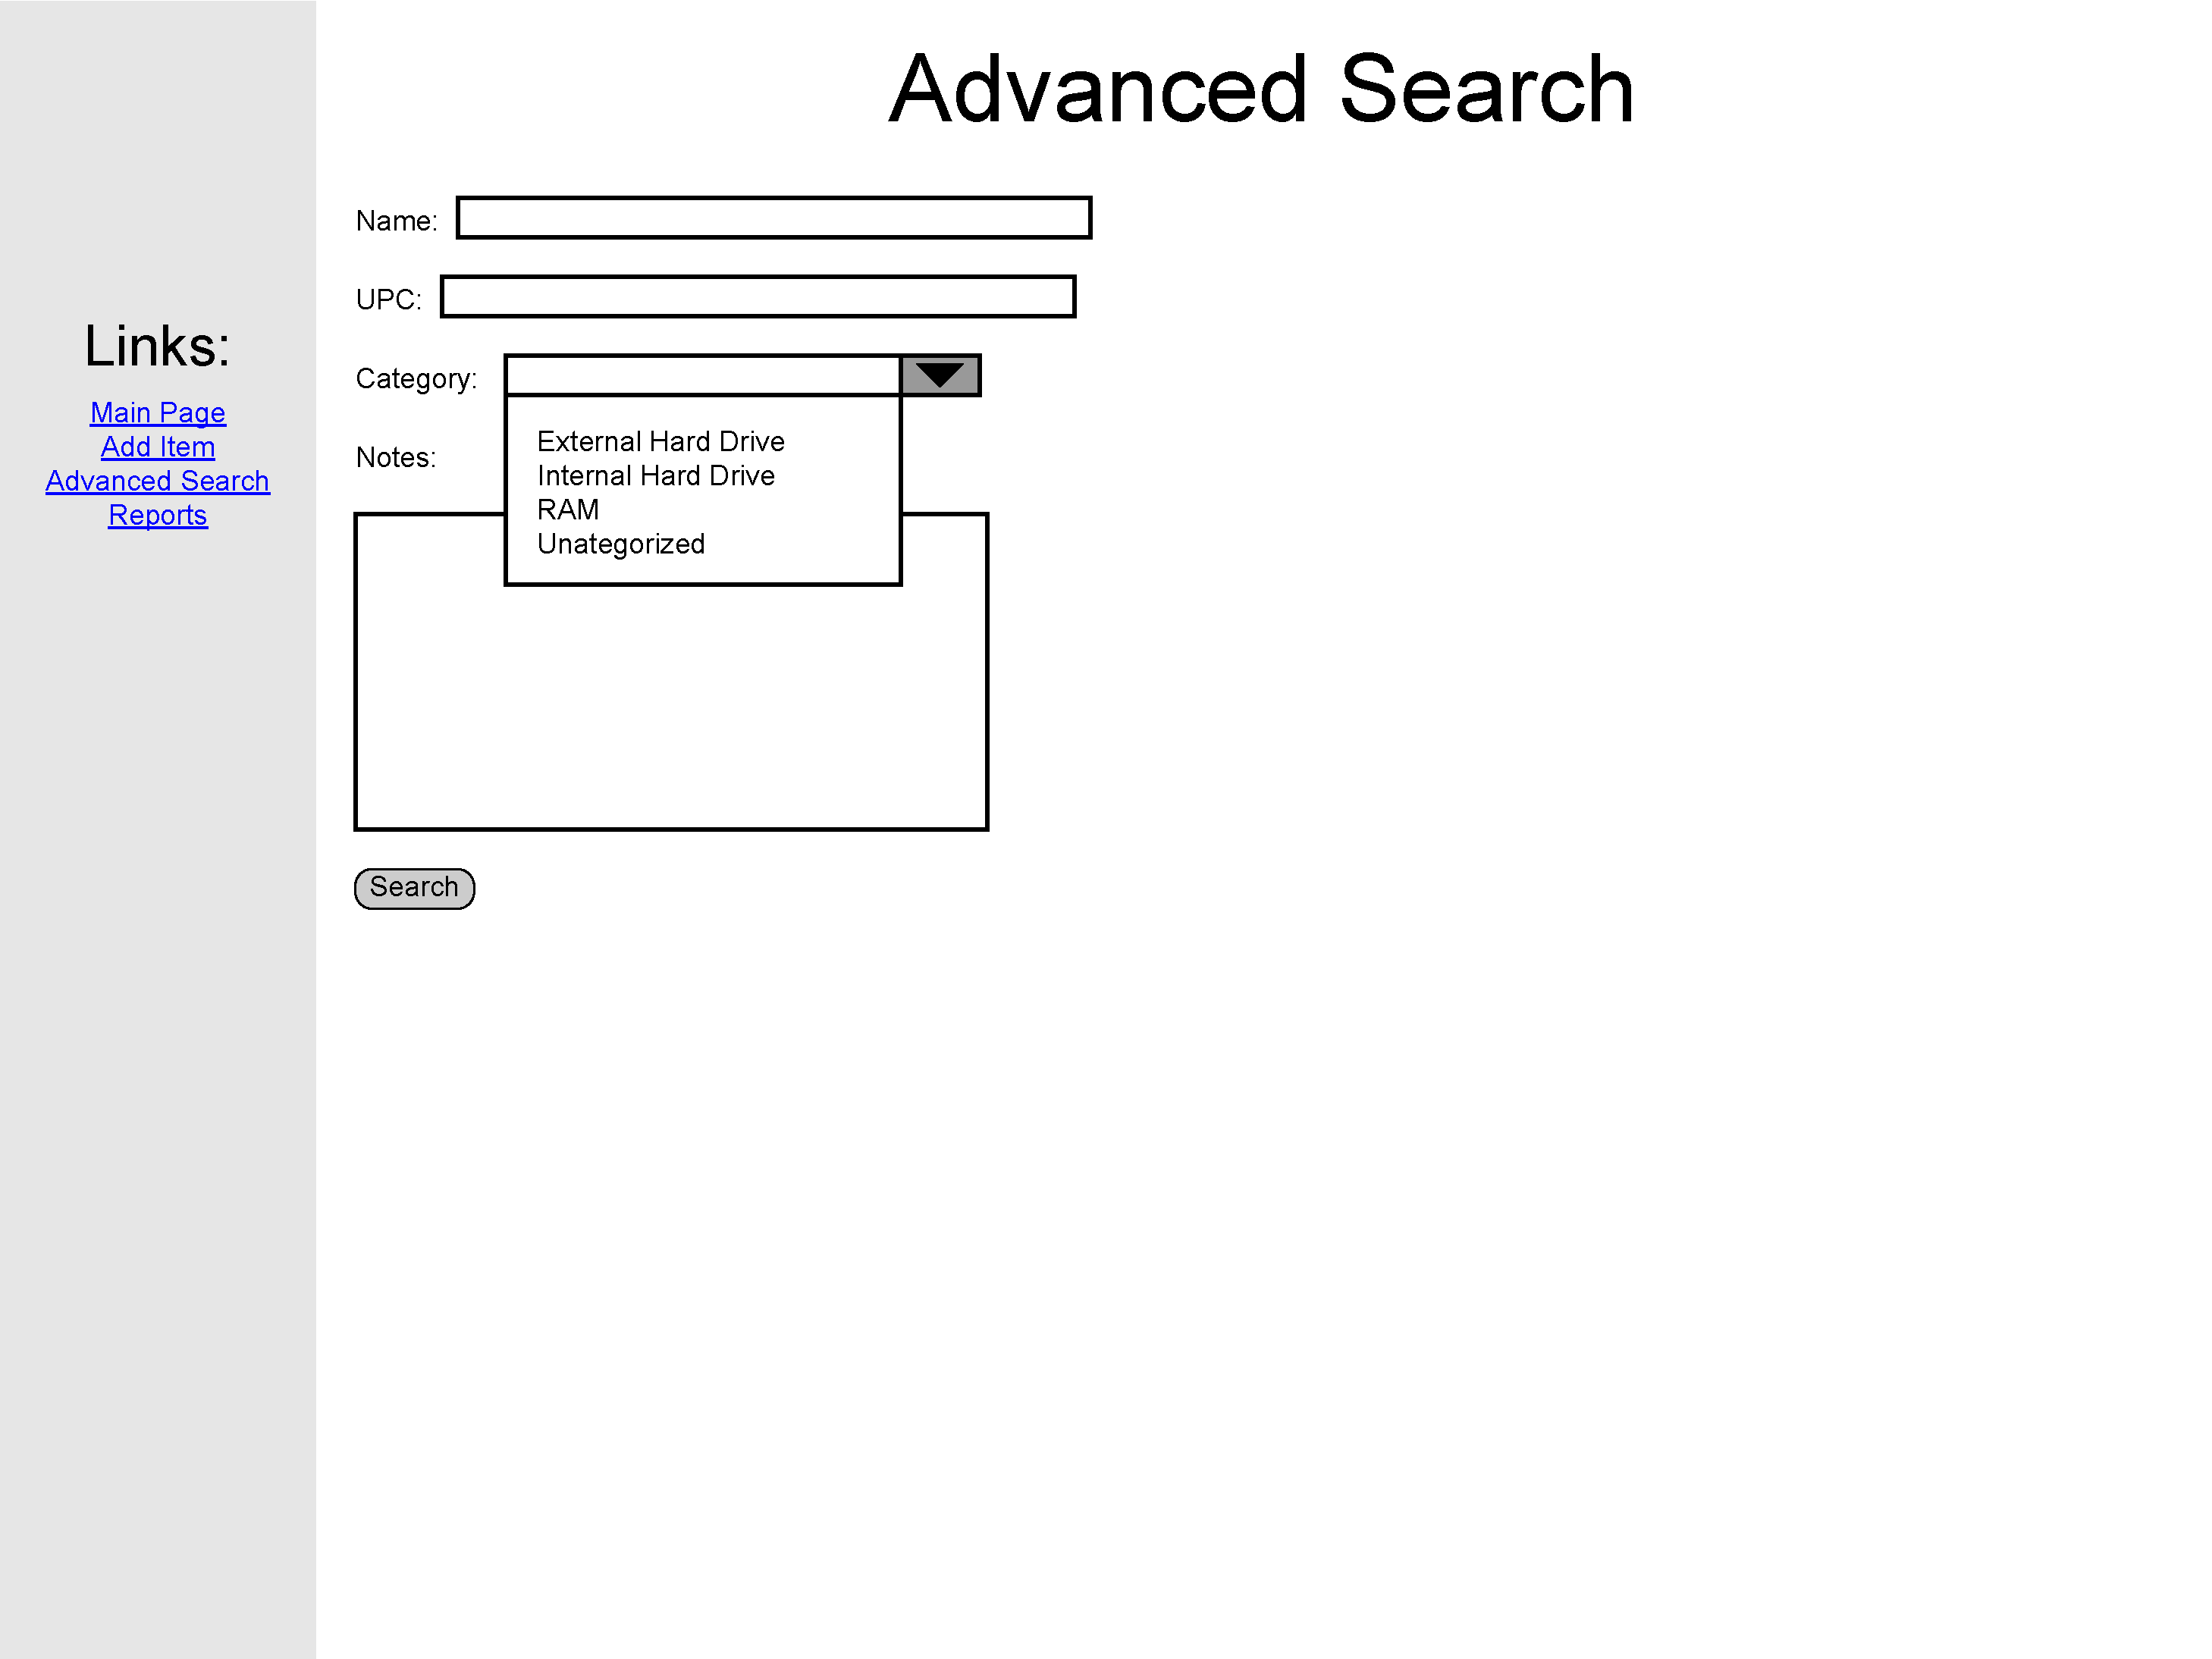
\includegraphics[keepaspectratio, width=4.5in]{advancedSearchF0S1.pdf} \\
The advanced search page with the category dropdown expanded
\end{tabular}\\
~\\
~\\
\begin{tabular}{ p{4.5in} }
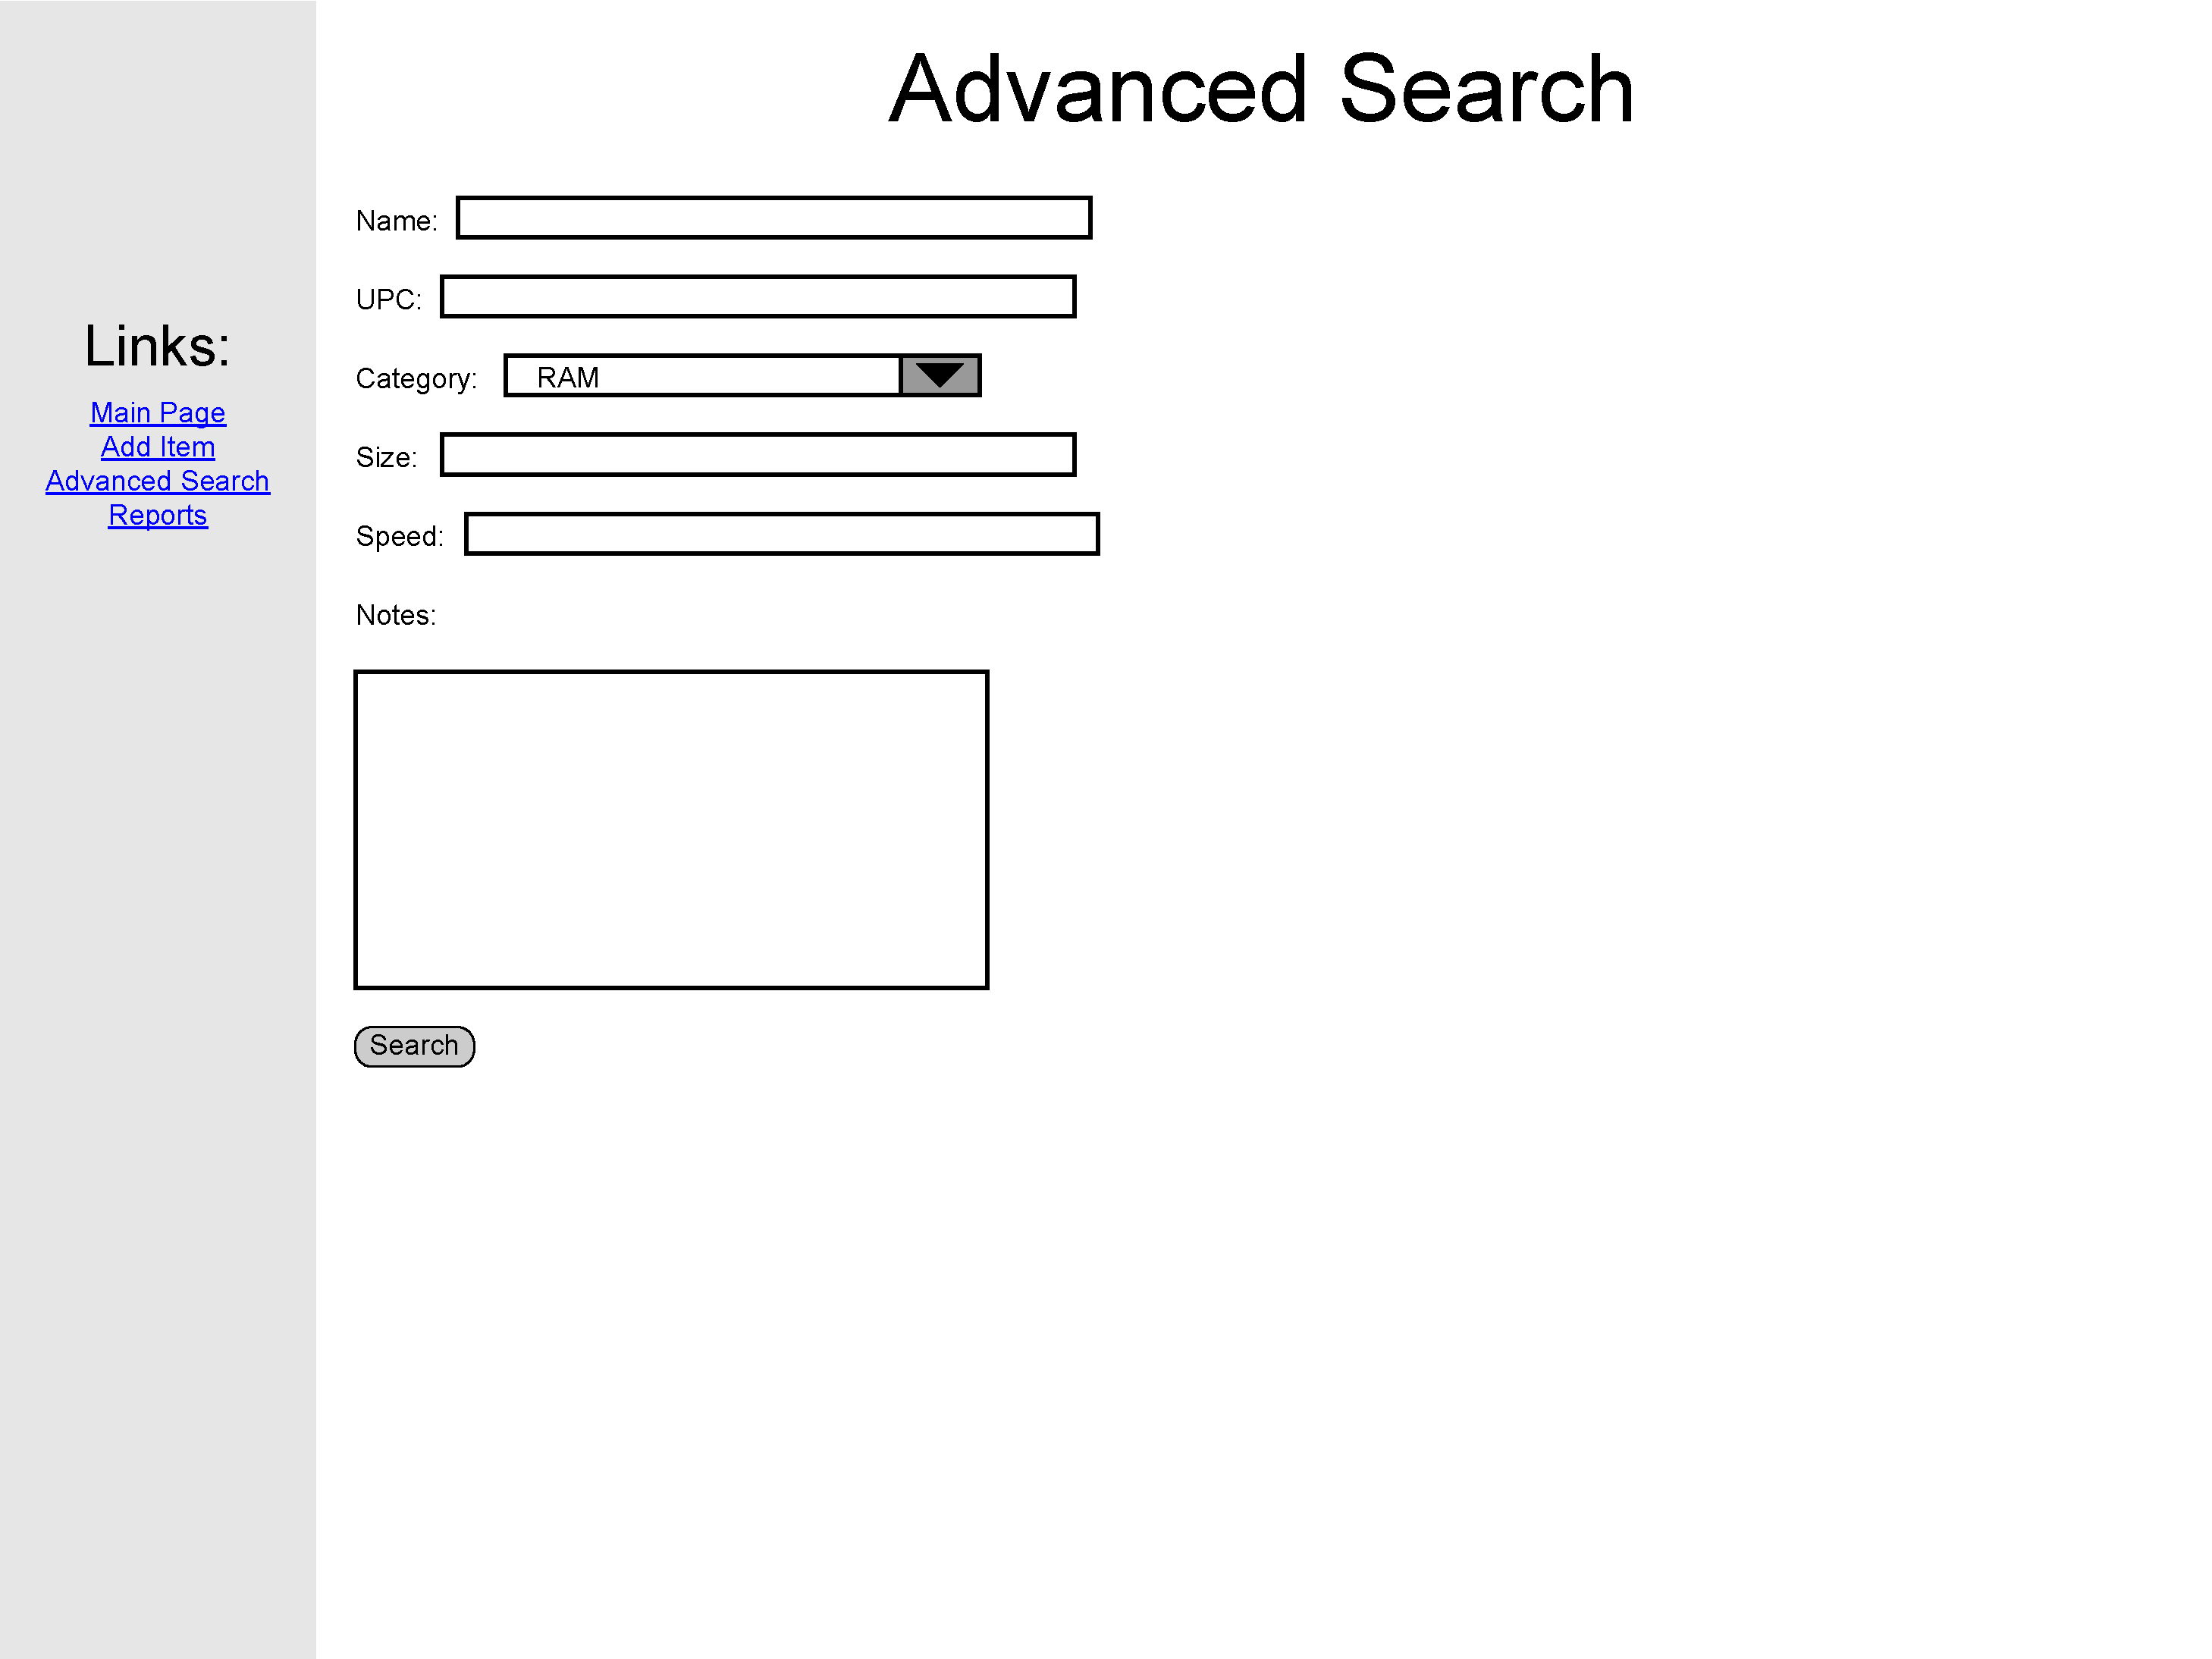
\includegraphics[keepaspectratio, width=4.5in]{advancedSearchF0S2.pdf} \\
The advanced search page with a category selected
\end{tabular}\\
~\\
~\\
\begin{tabular}{ p{4.5in} }
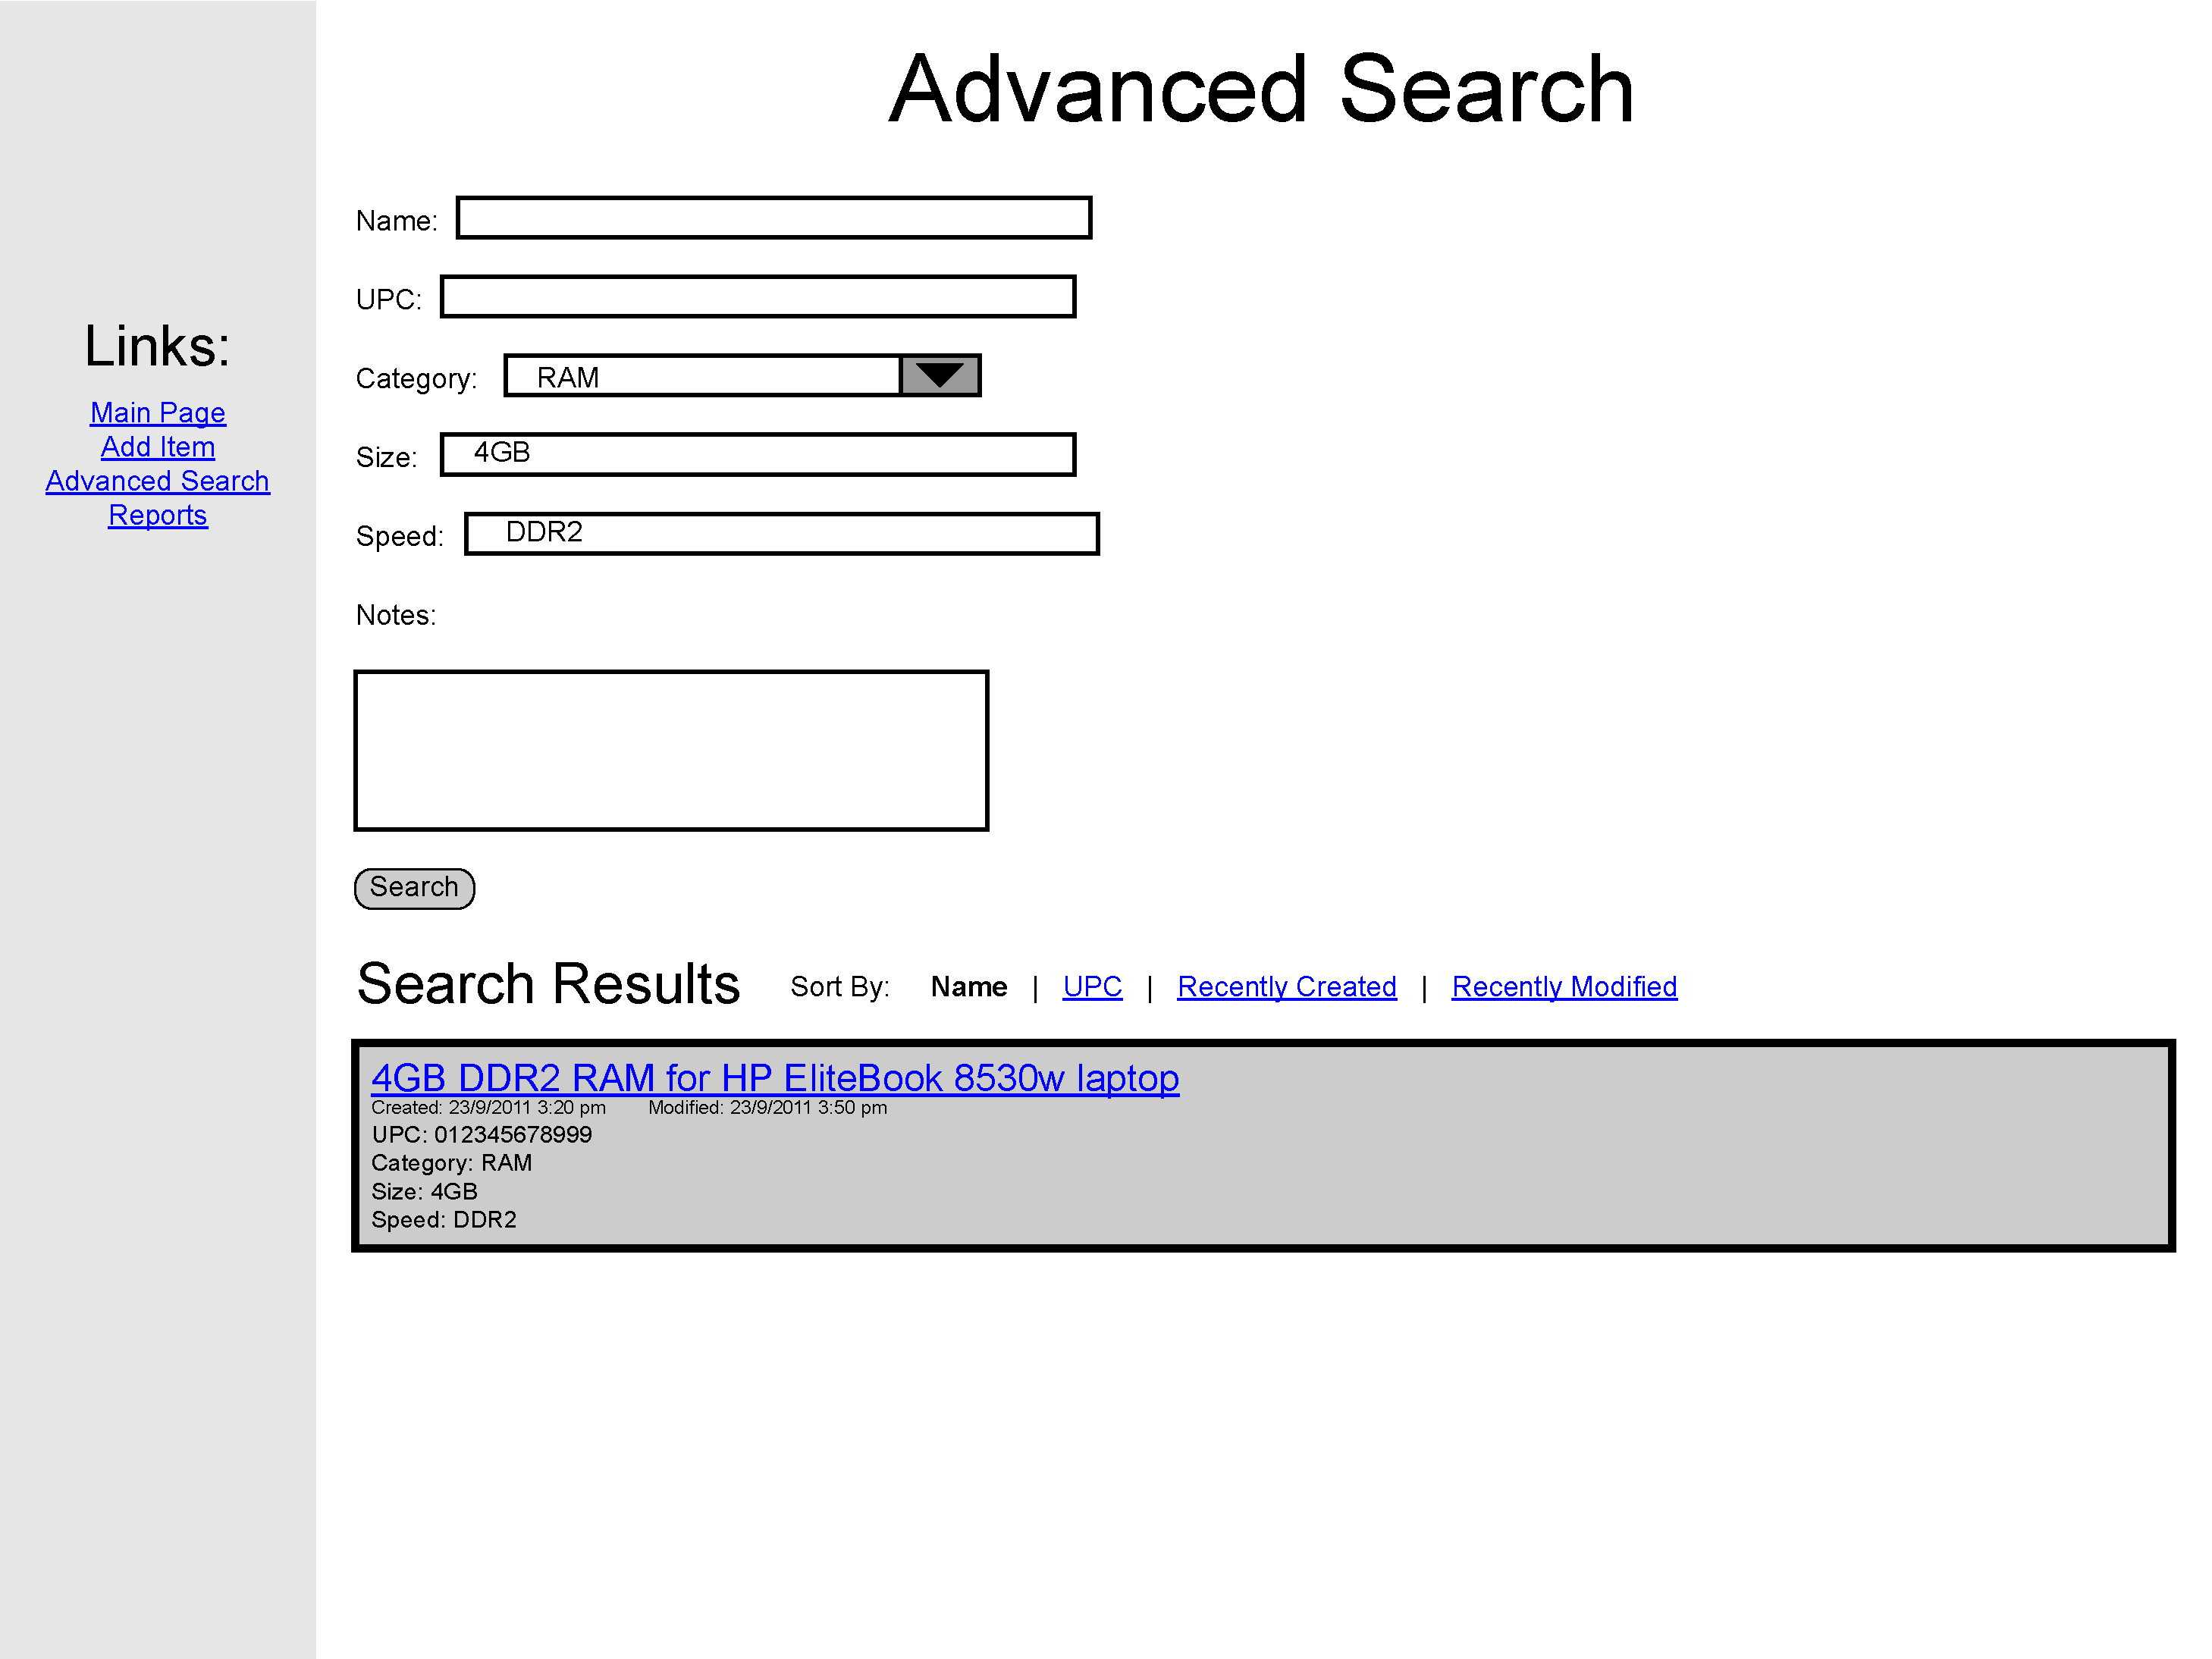
\includegraphics[keepaspectratio, width=4.5in]{advancedSearchF0S3.pdf} \\
The advanced search page with results showing
\end{tabular}\\
~\\
~\\
\begin{tabular}{ p{4.5in} }
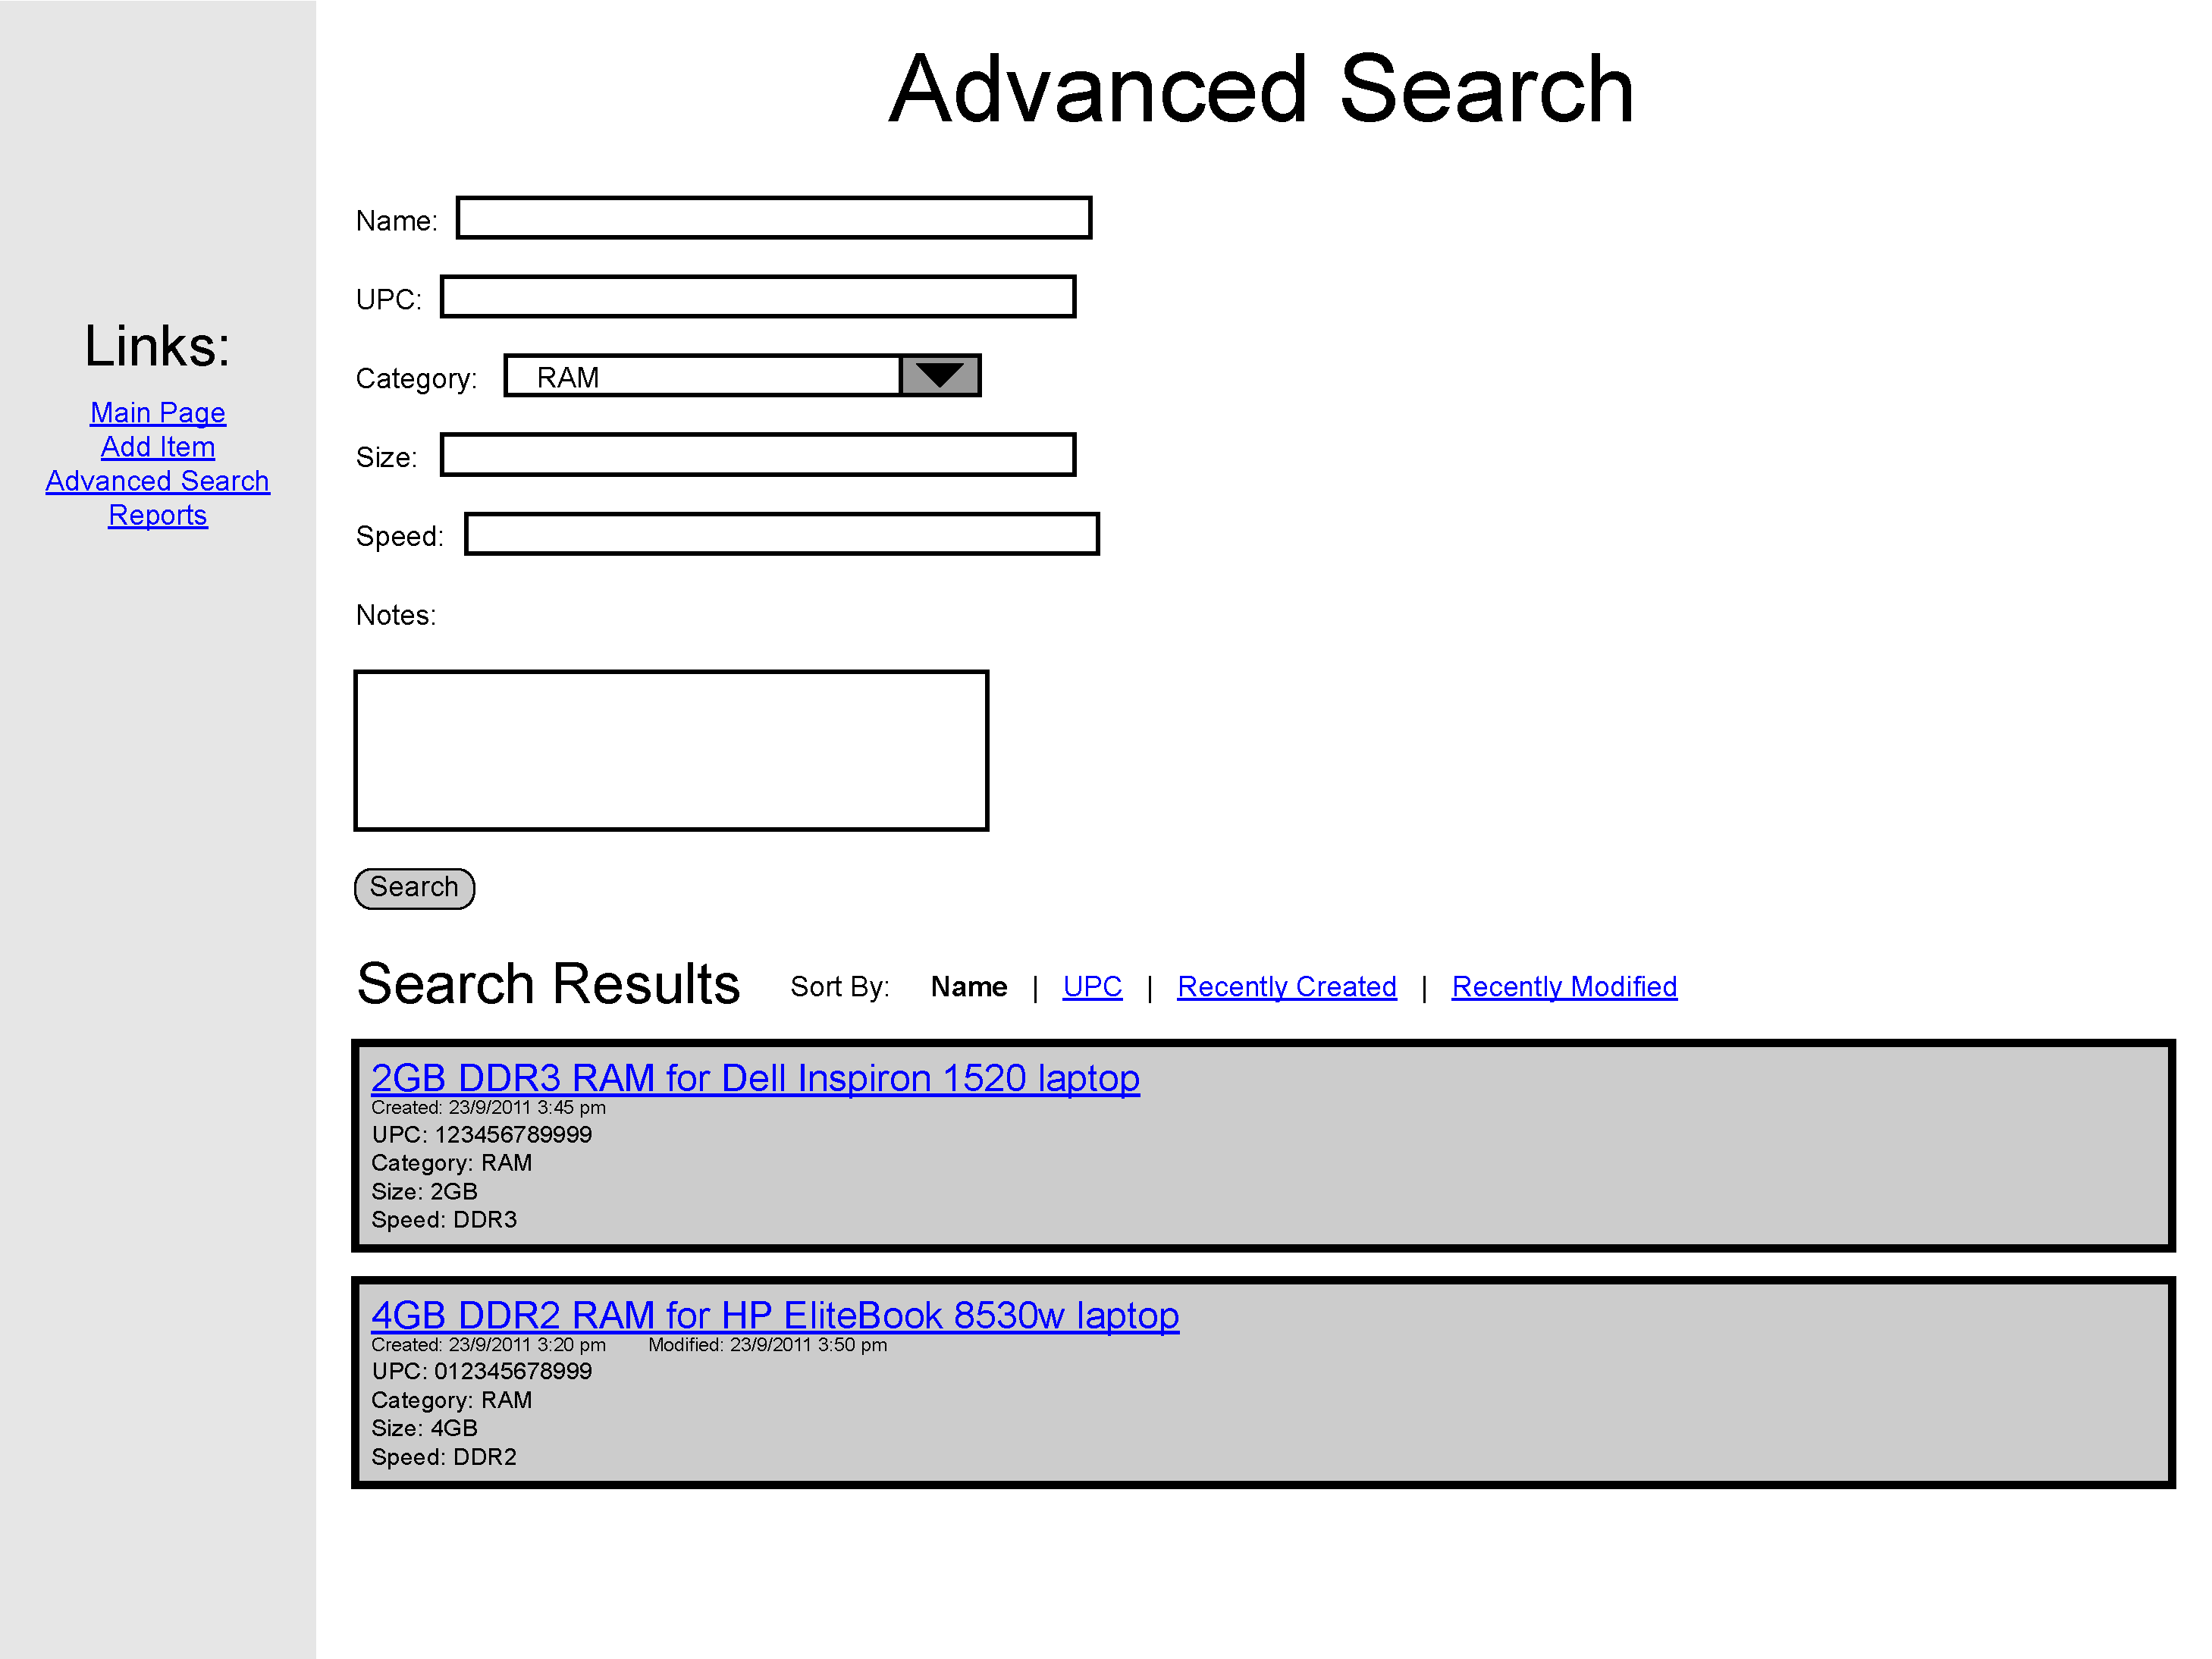
\includegraphics[keepaspectratio, width=4.5in]{sortResultsF0S0.pdf} \\
The advanced search page with results sorted by the default of Name
\end{tabular}\\
~\\
~\\
\begin{tabular}{ p{4.5in} }
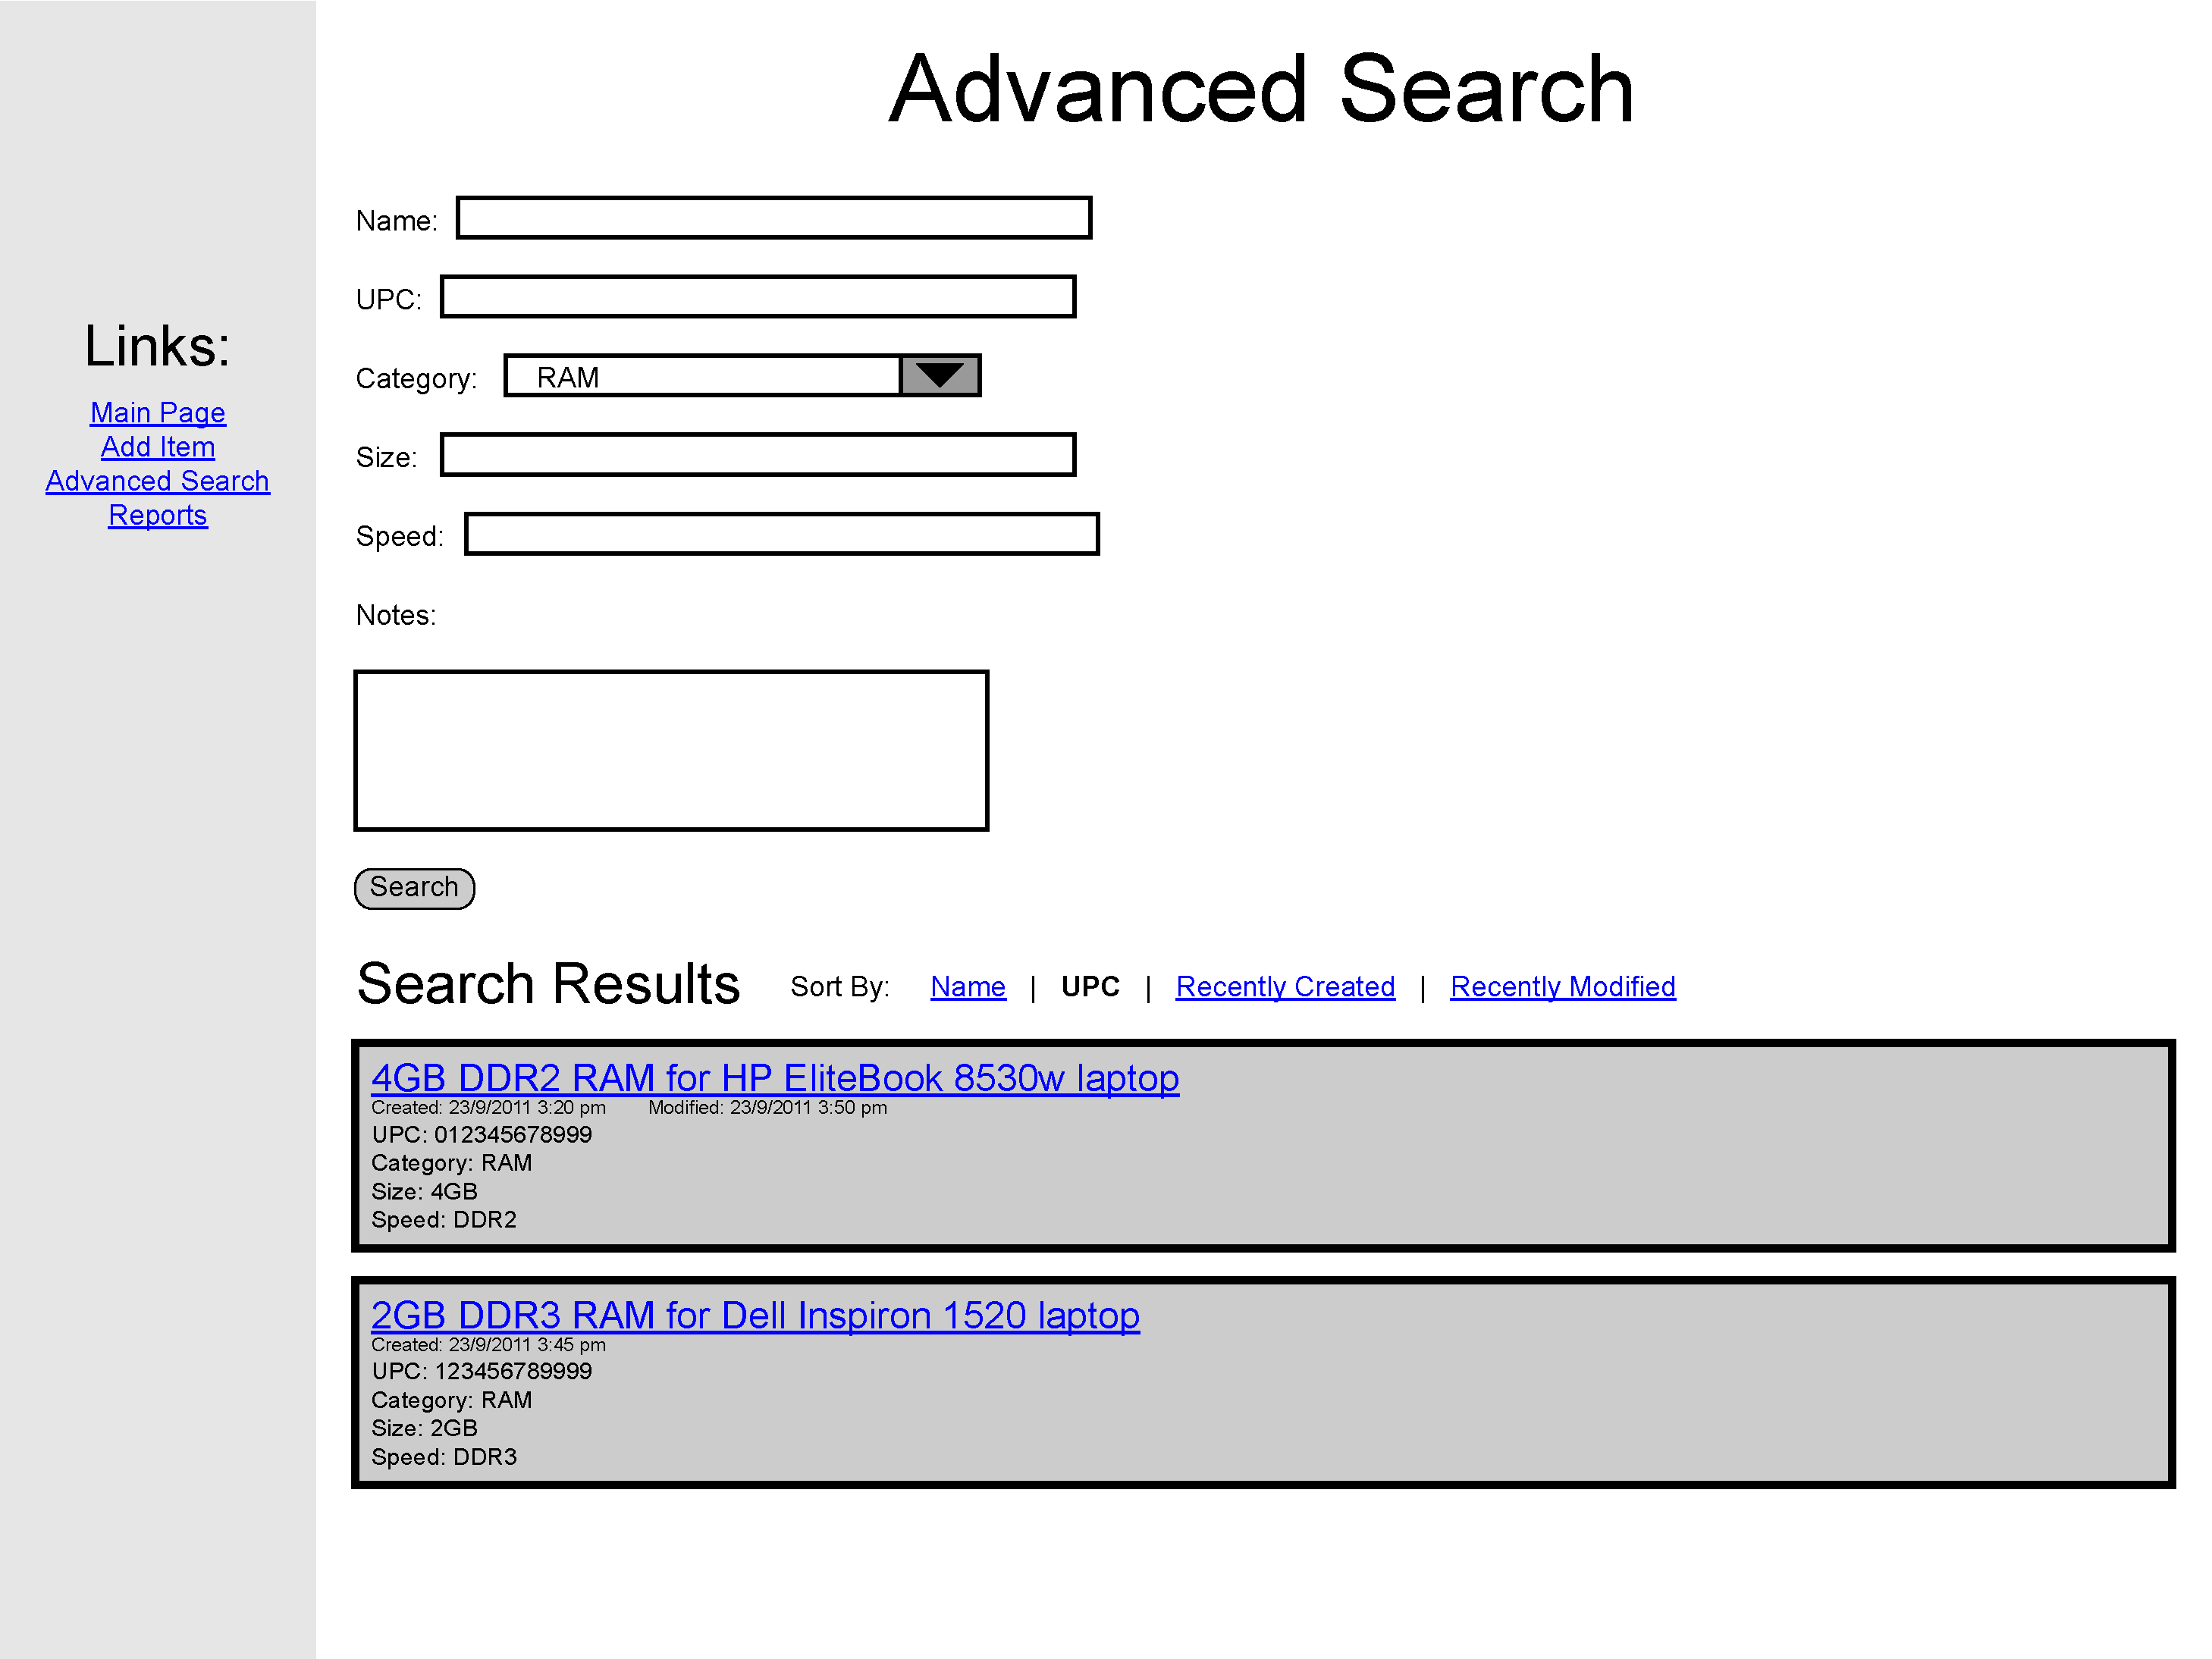
\includegraphics[keepaspectratio, width=4.5in]{sortResultsF0S1.pdf} \\
The advanced search page with results sorted by the user's choice of UPC
\end{tabular}\\
~\\
~\\
\begin{tabular}{ p{4.5in} }
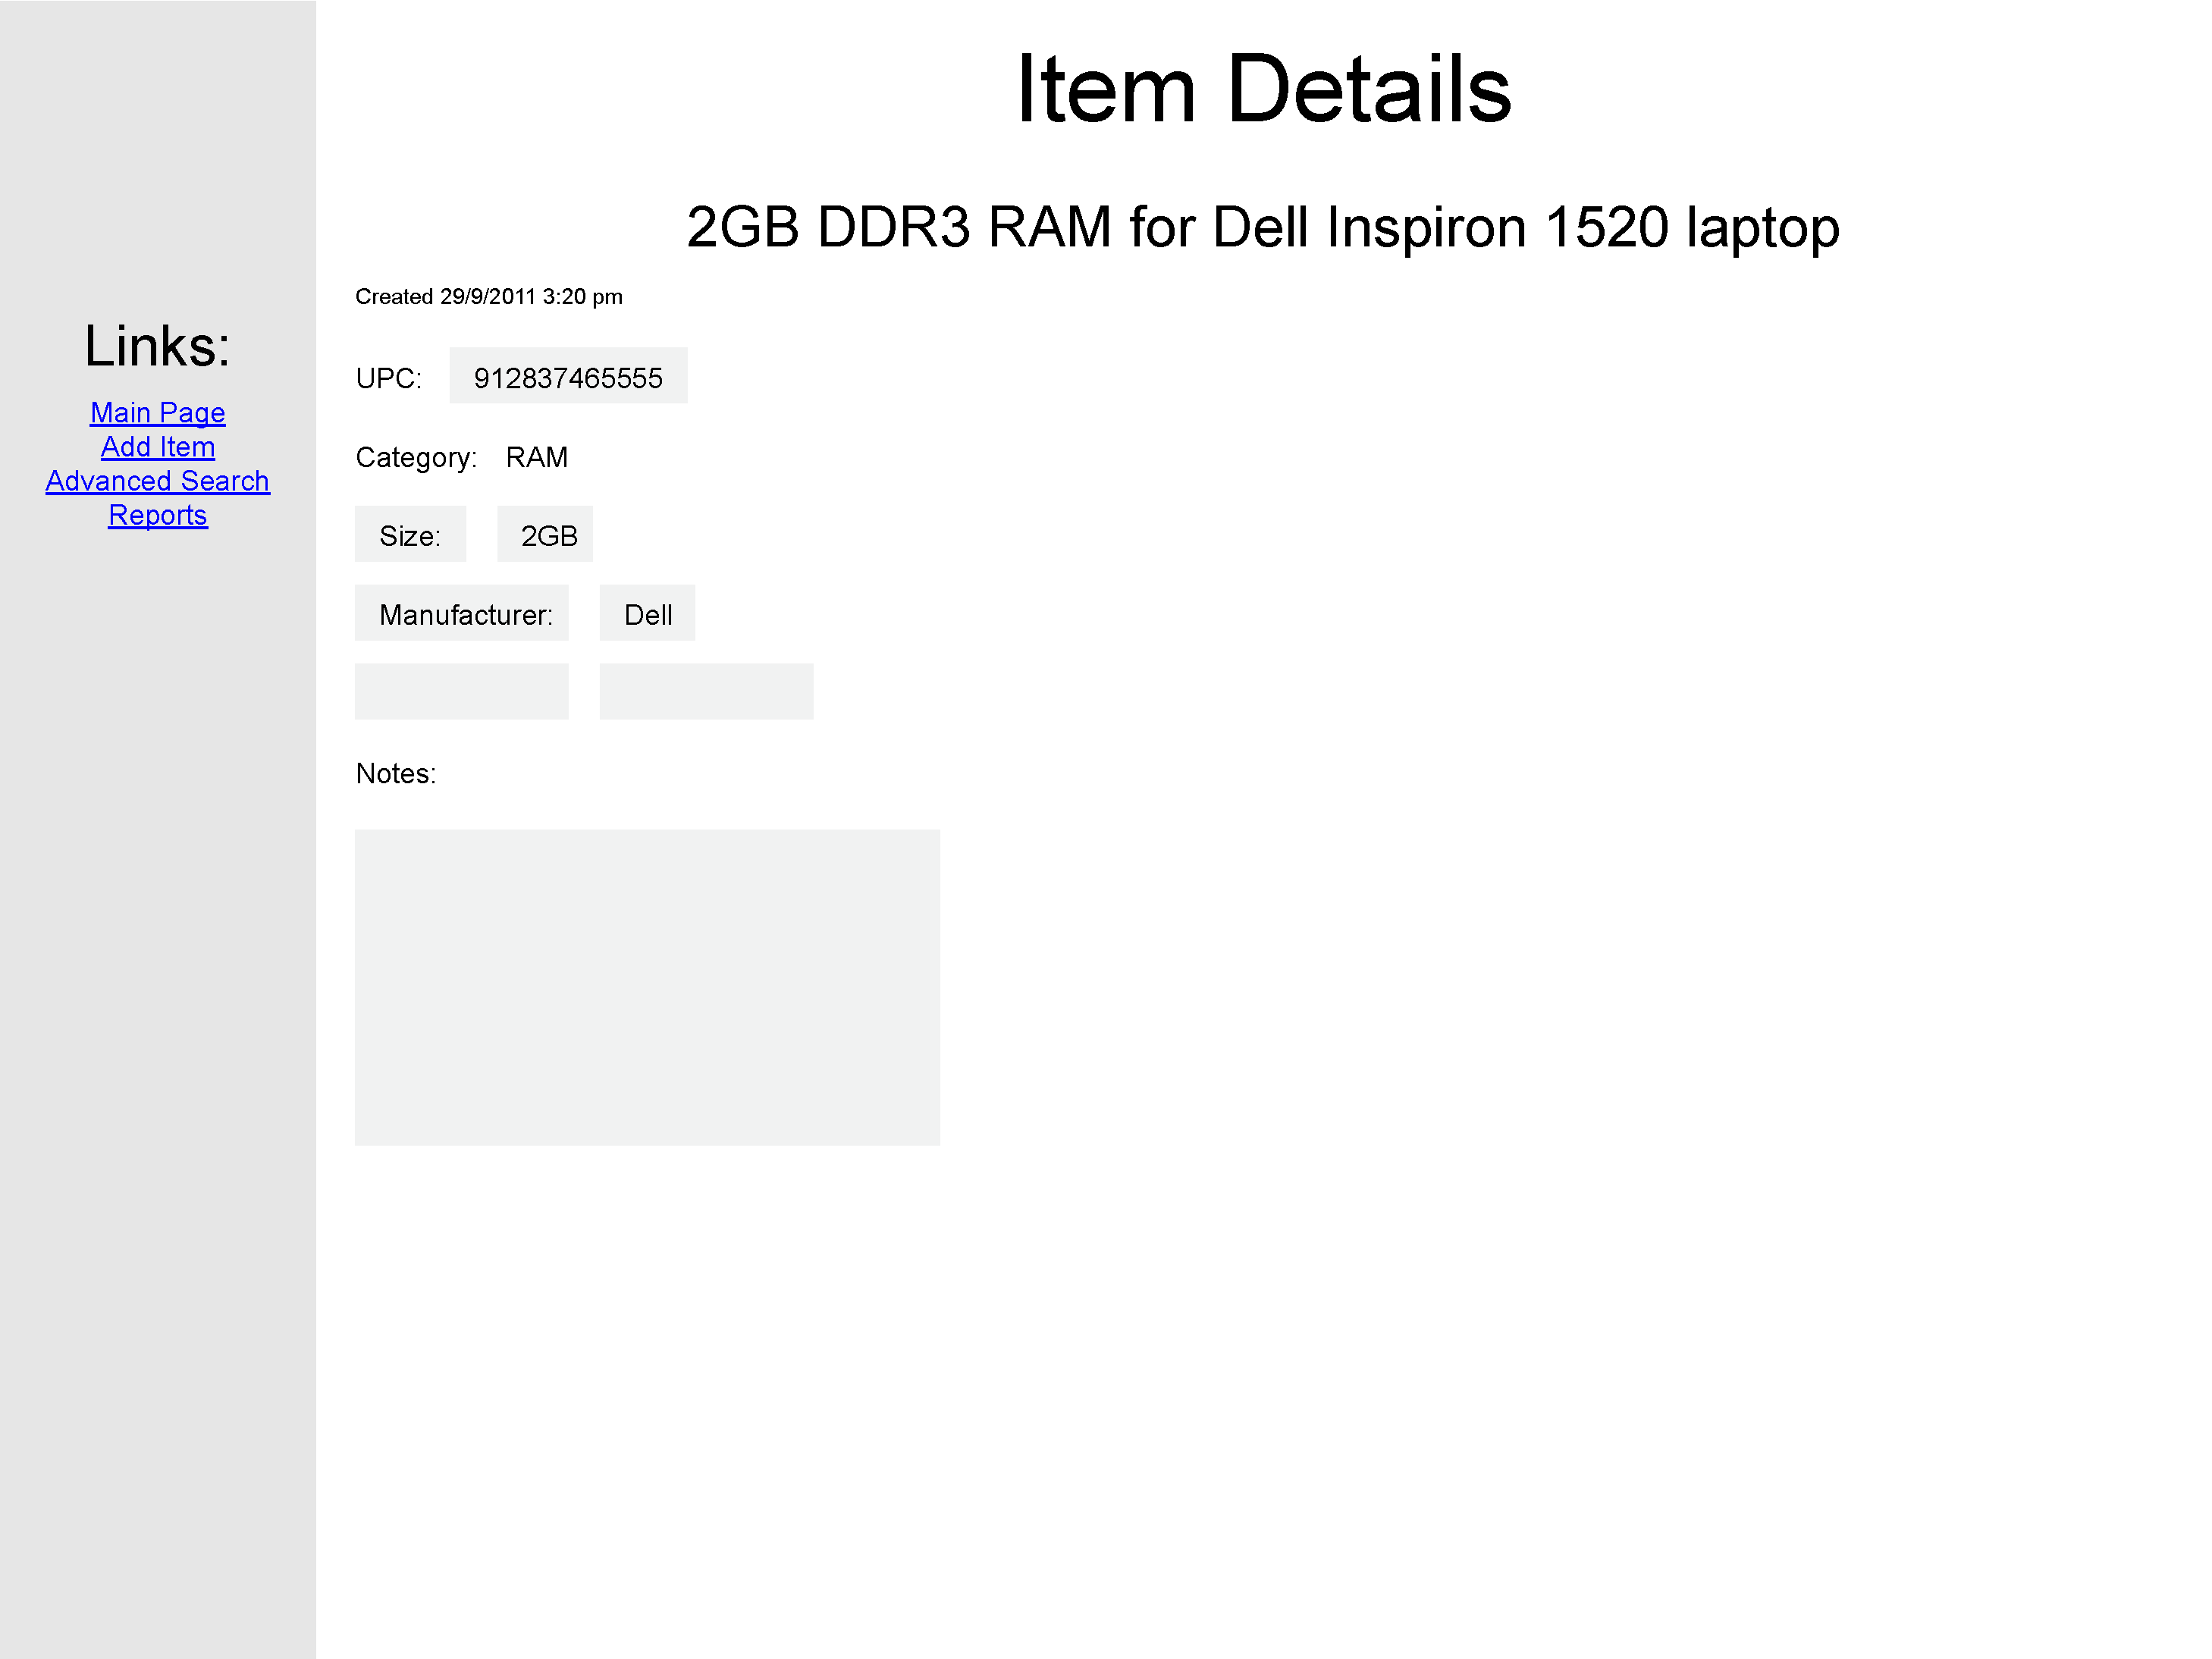
\includegraphics[keepaspectratio, width=4.5in]{viewDetailsF0S1.pdf} \\
The item details page in its initial state
\end{tabular}\\
~\\
~\\
\begin{tabular}{ p{4.5in} }
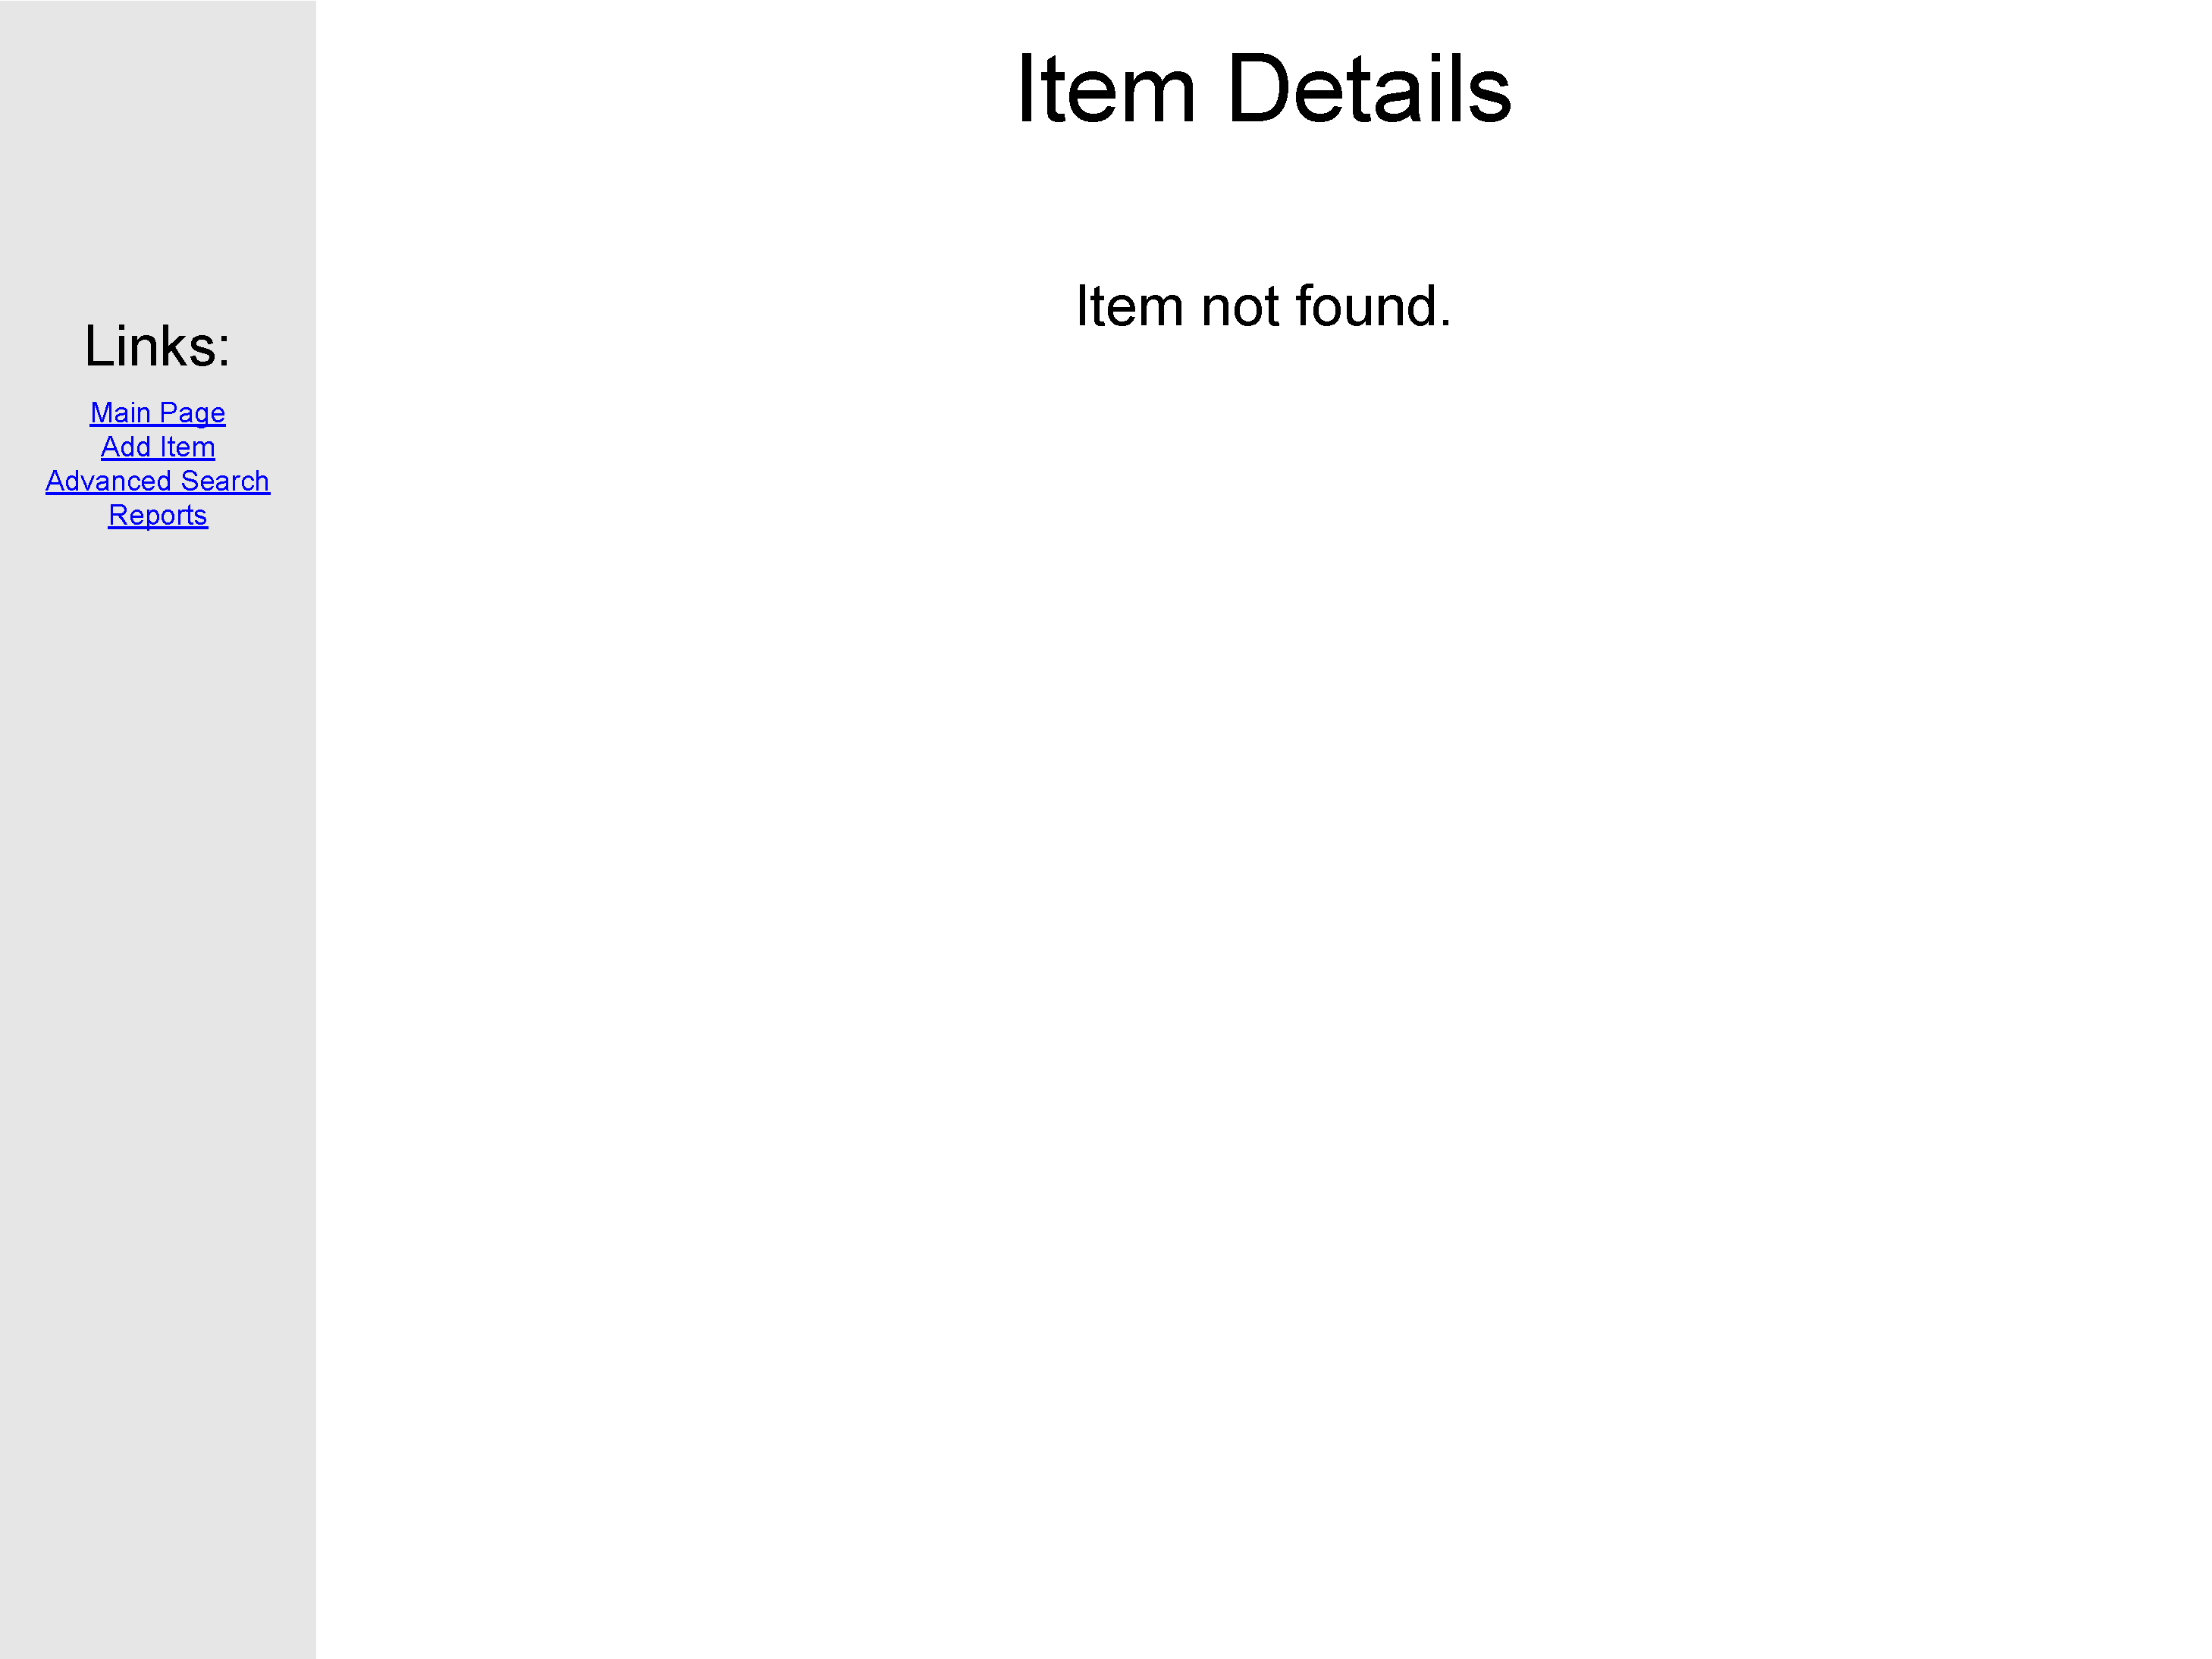
\includegraphics[keepaspectratio, width=4.5in]{viewDetailsF1S1.pdf} \\
The item details page for an item that could not be found.
\end{tabular}\\
~\\
~\\
\begin{tabular}{ p{4.5in} }
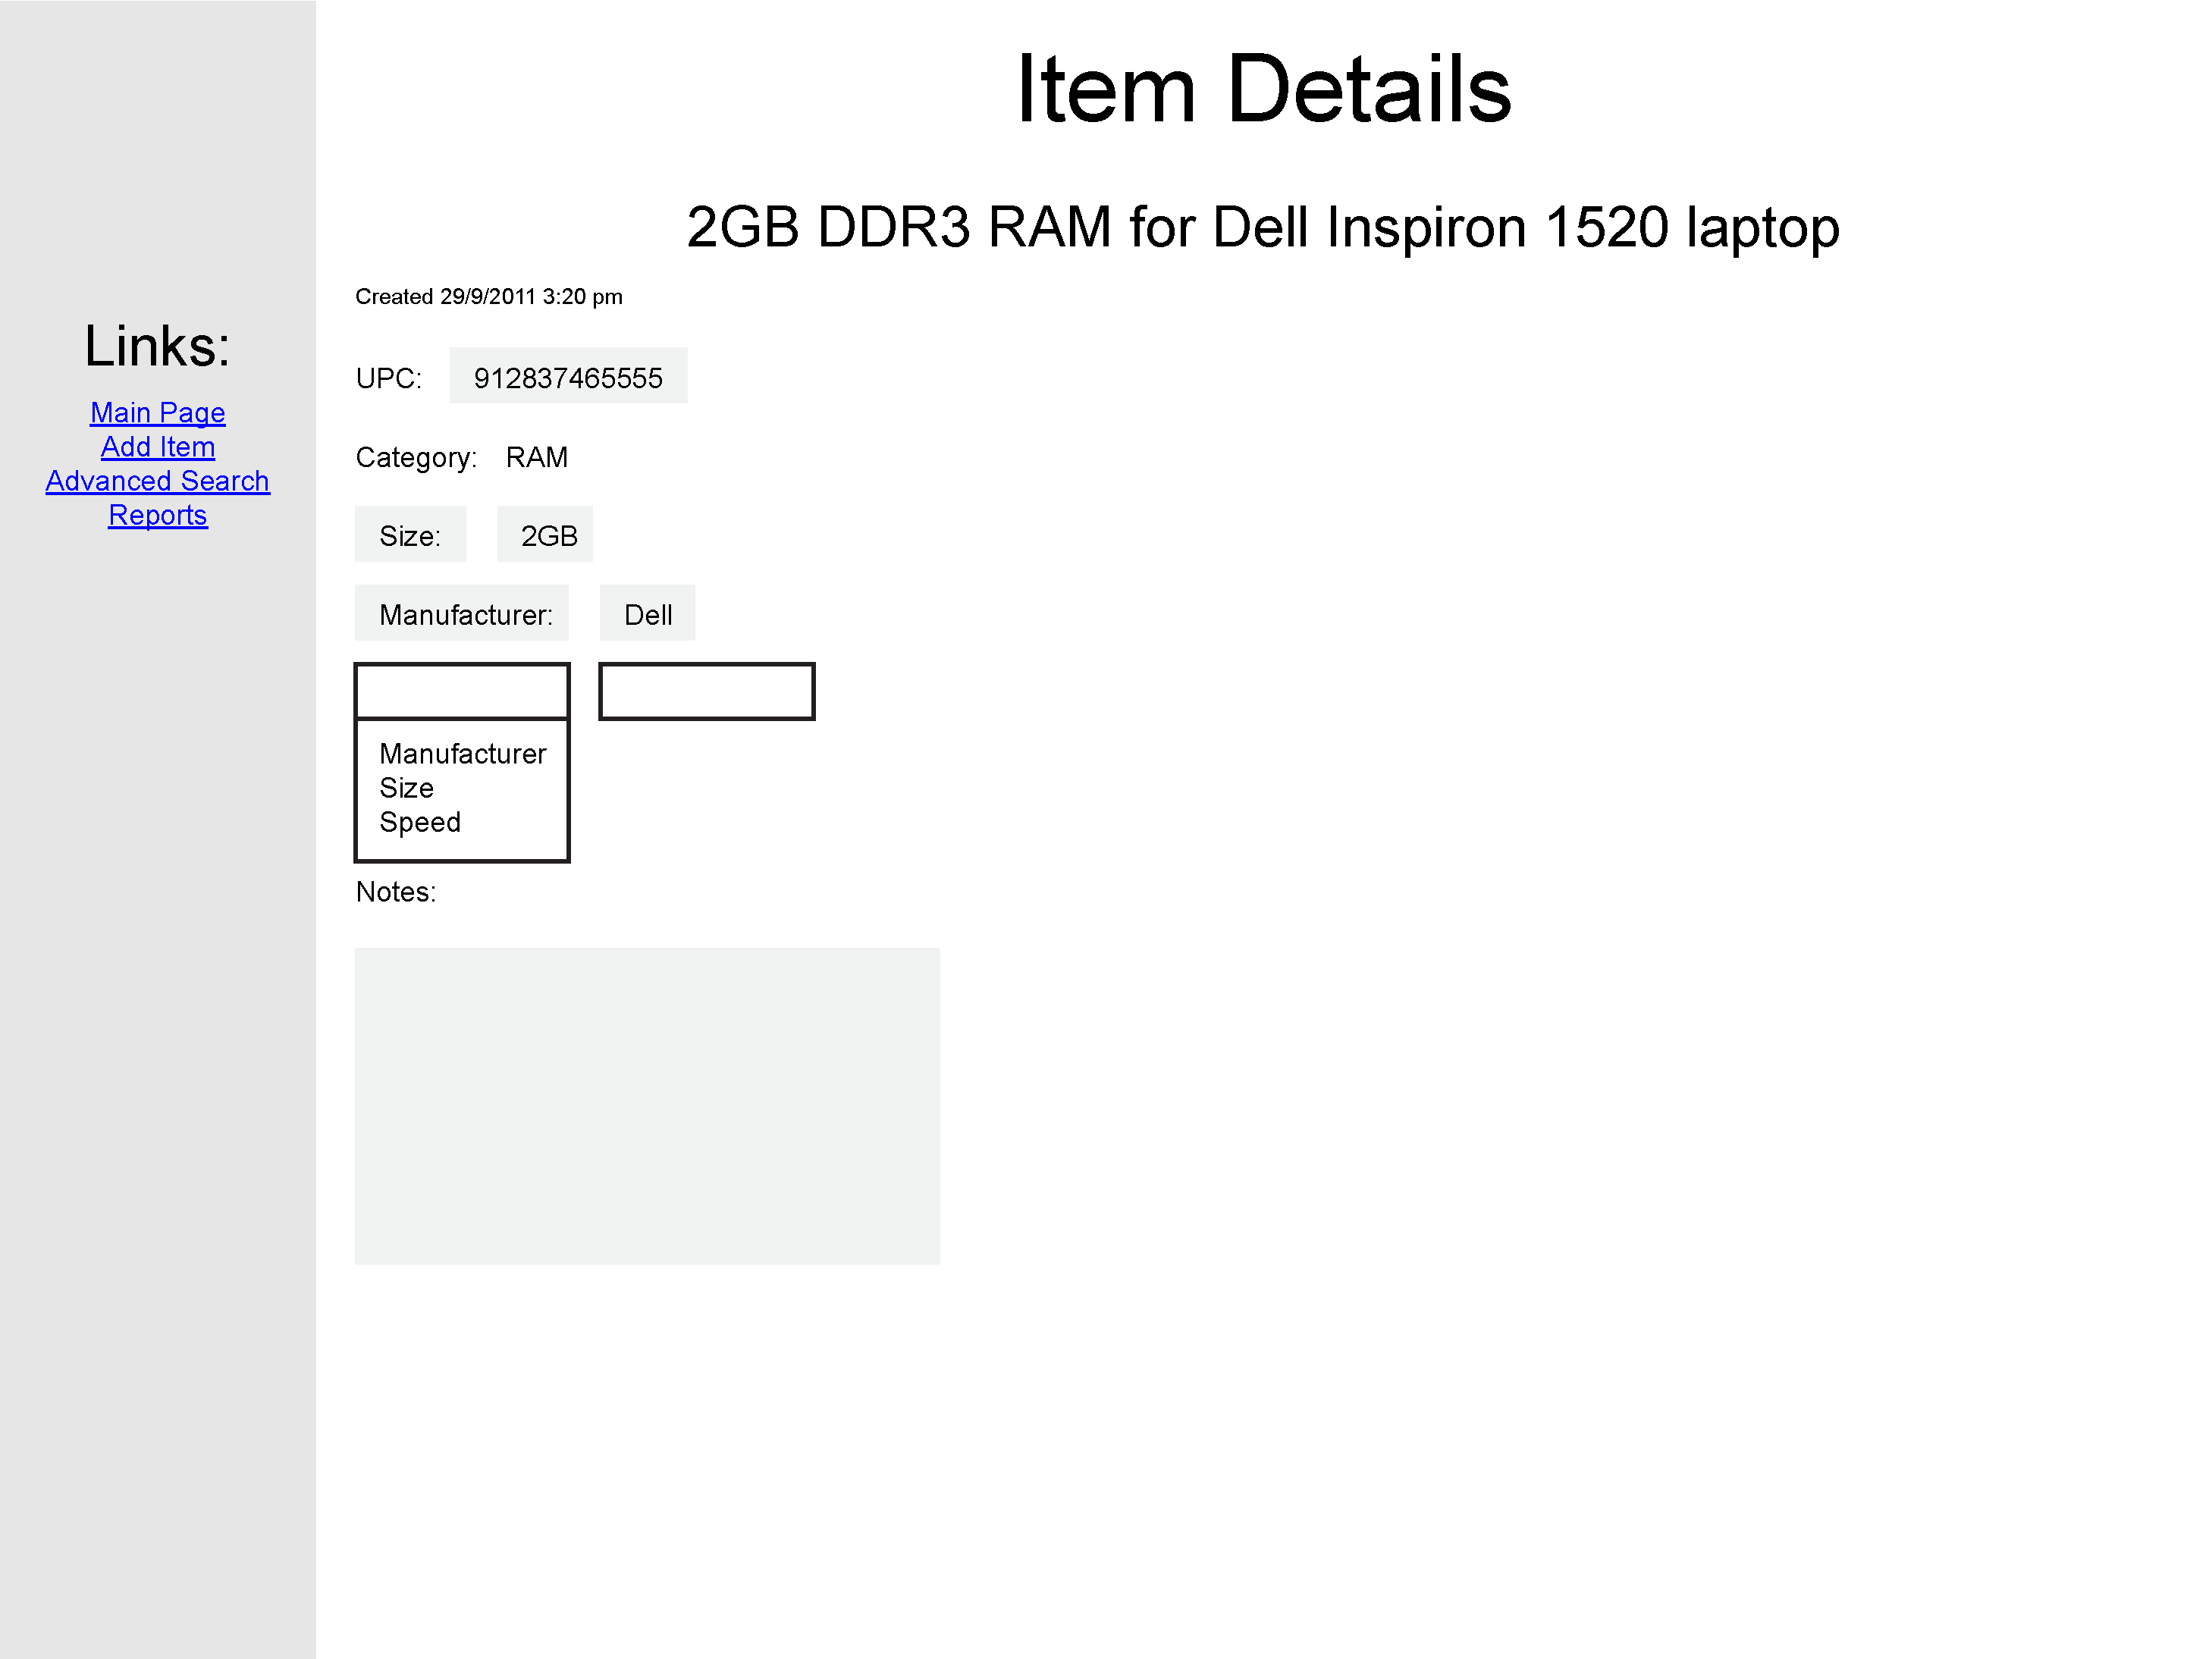
\includegraphics[keepaspectratio, width=4.5in]{modifyDetailsF0S1.pdf} \\
The item details page after the user has clicked on the empty attribute key field and caused the element to be replaced with an autocomplete text field
\end{tabular}\\
~\\
~\\
\begin{tabular}{ p{4.5in} }
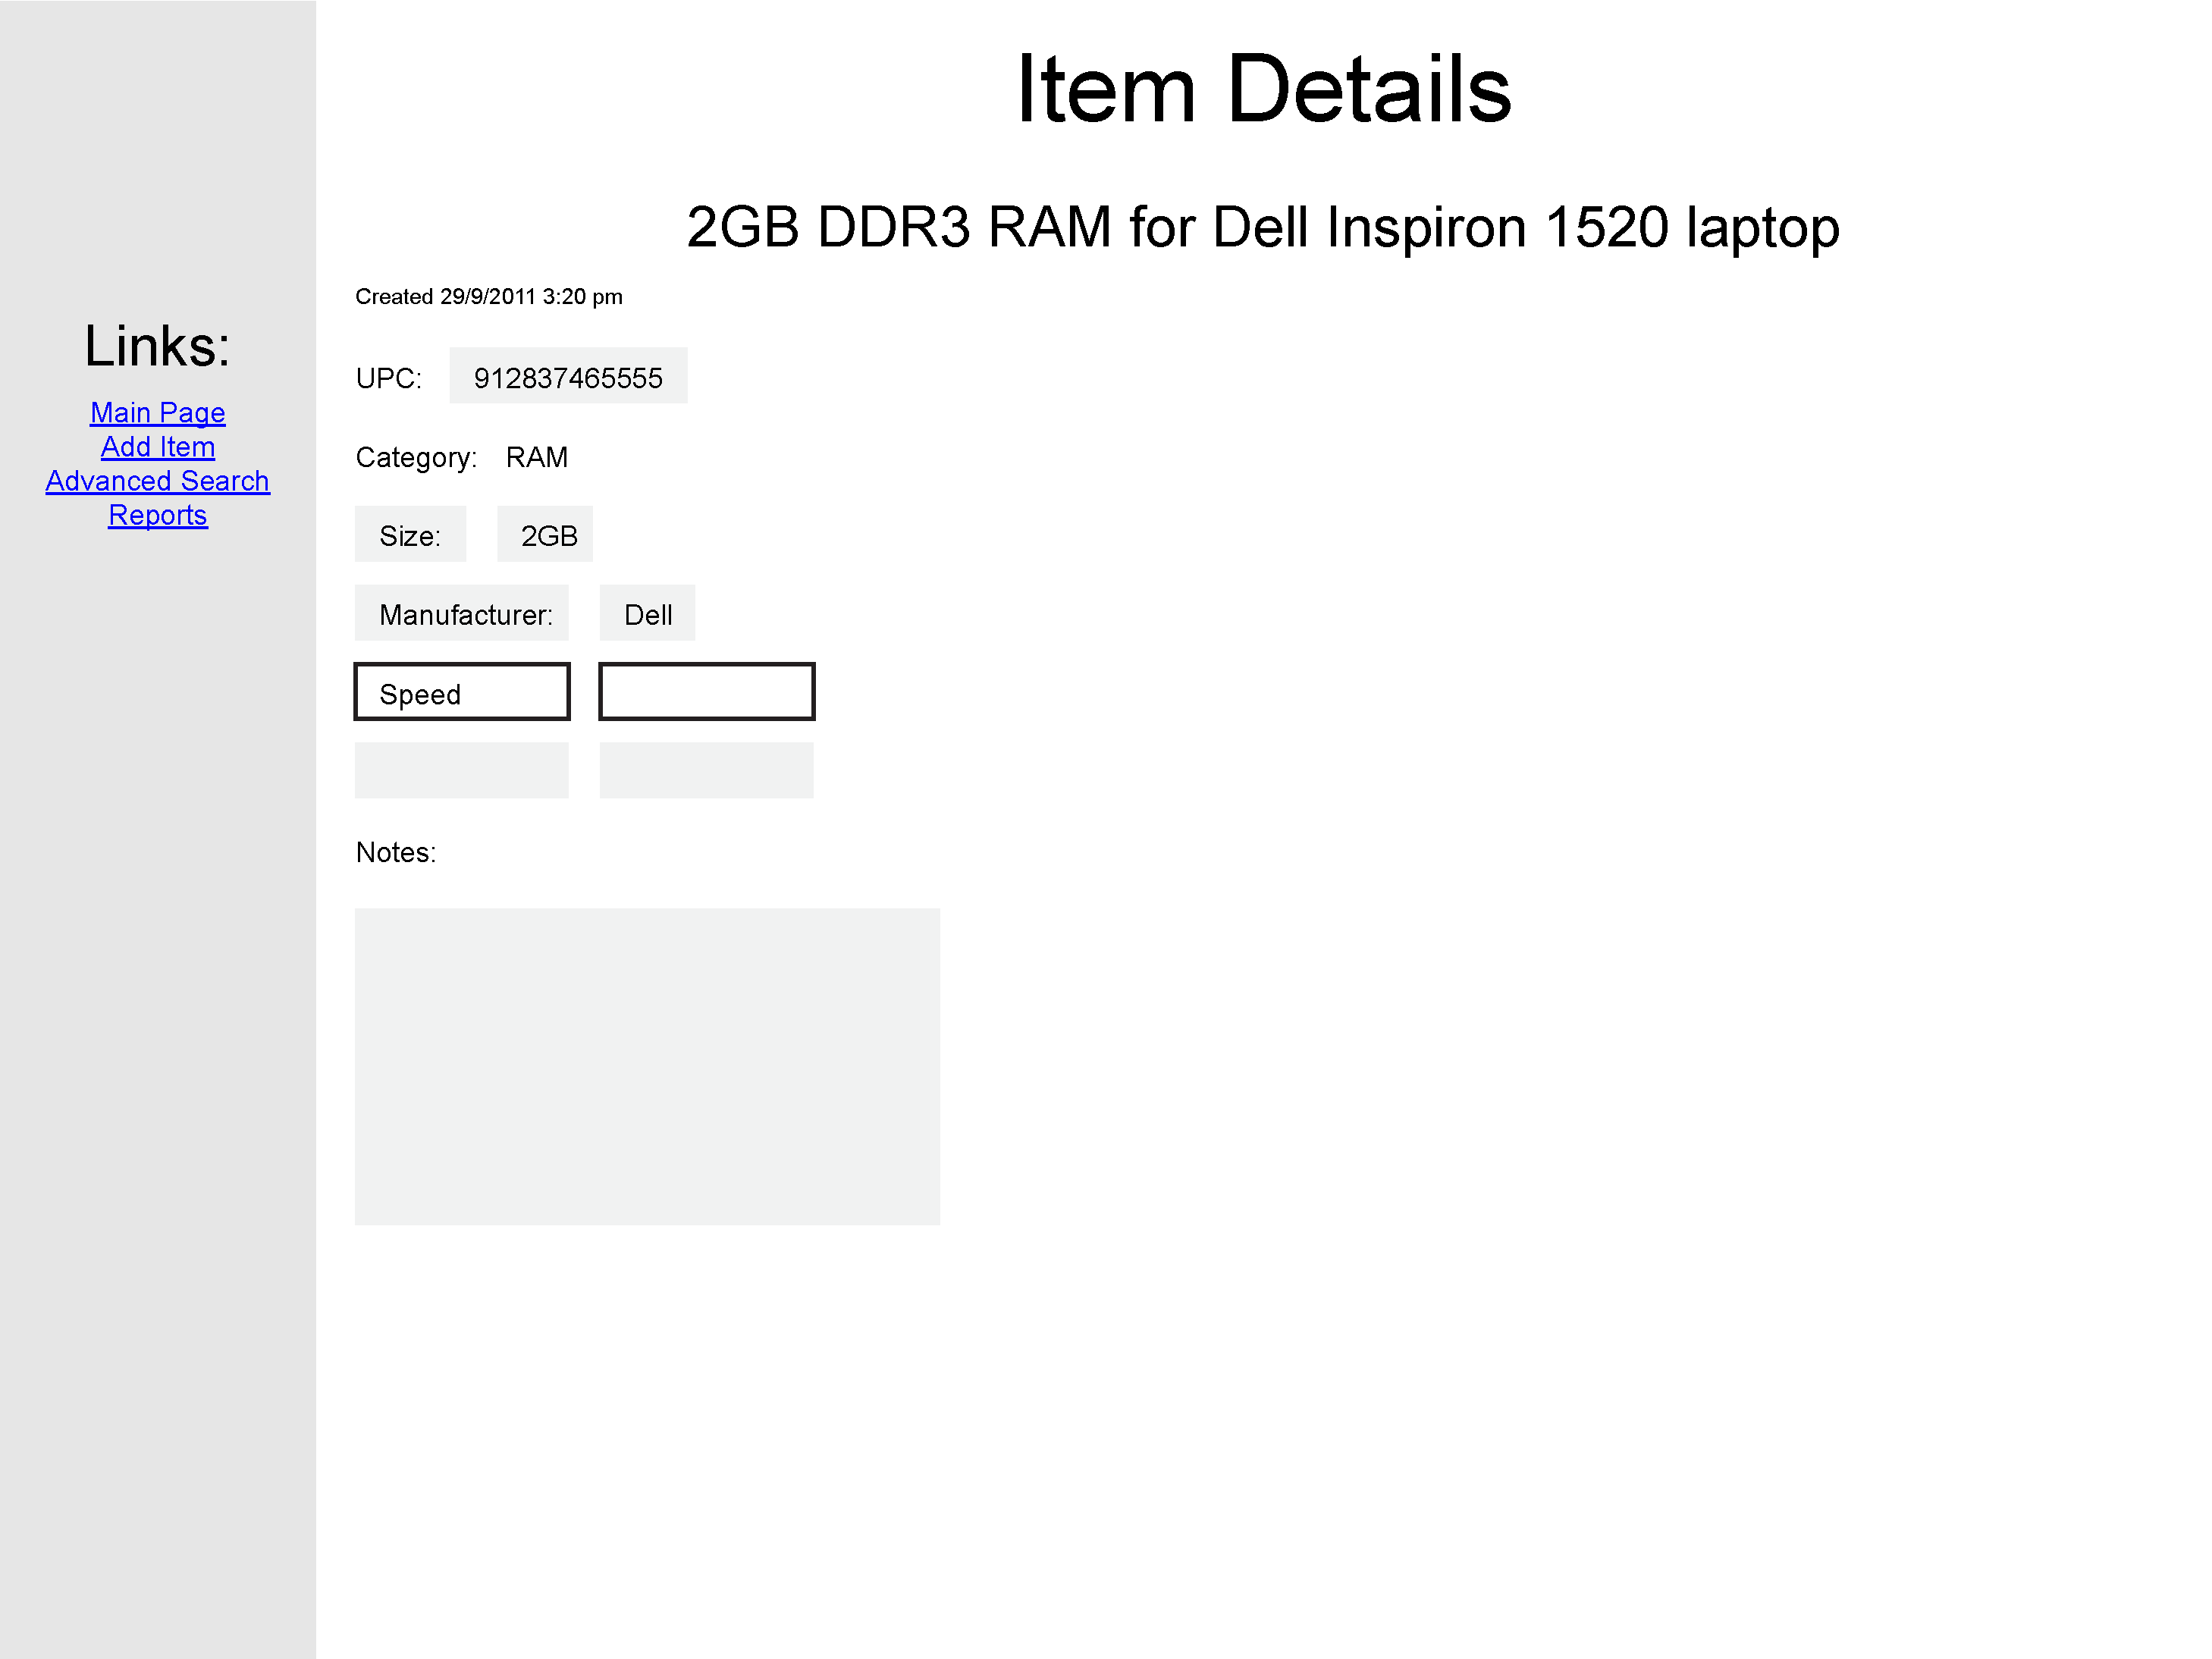
\includegraphics[keepaspectratio, width=4.5in]{modifyDetailsF0S2.pdf} \\
The item details page after an attribute key has been selected
\end{tabular}\\
~\\
~\\
\begin{tabular}{ p{4.5in} }
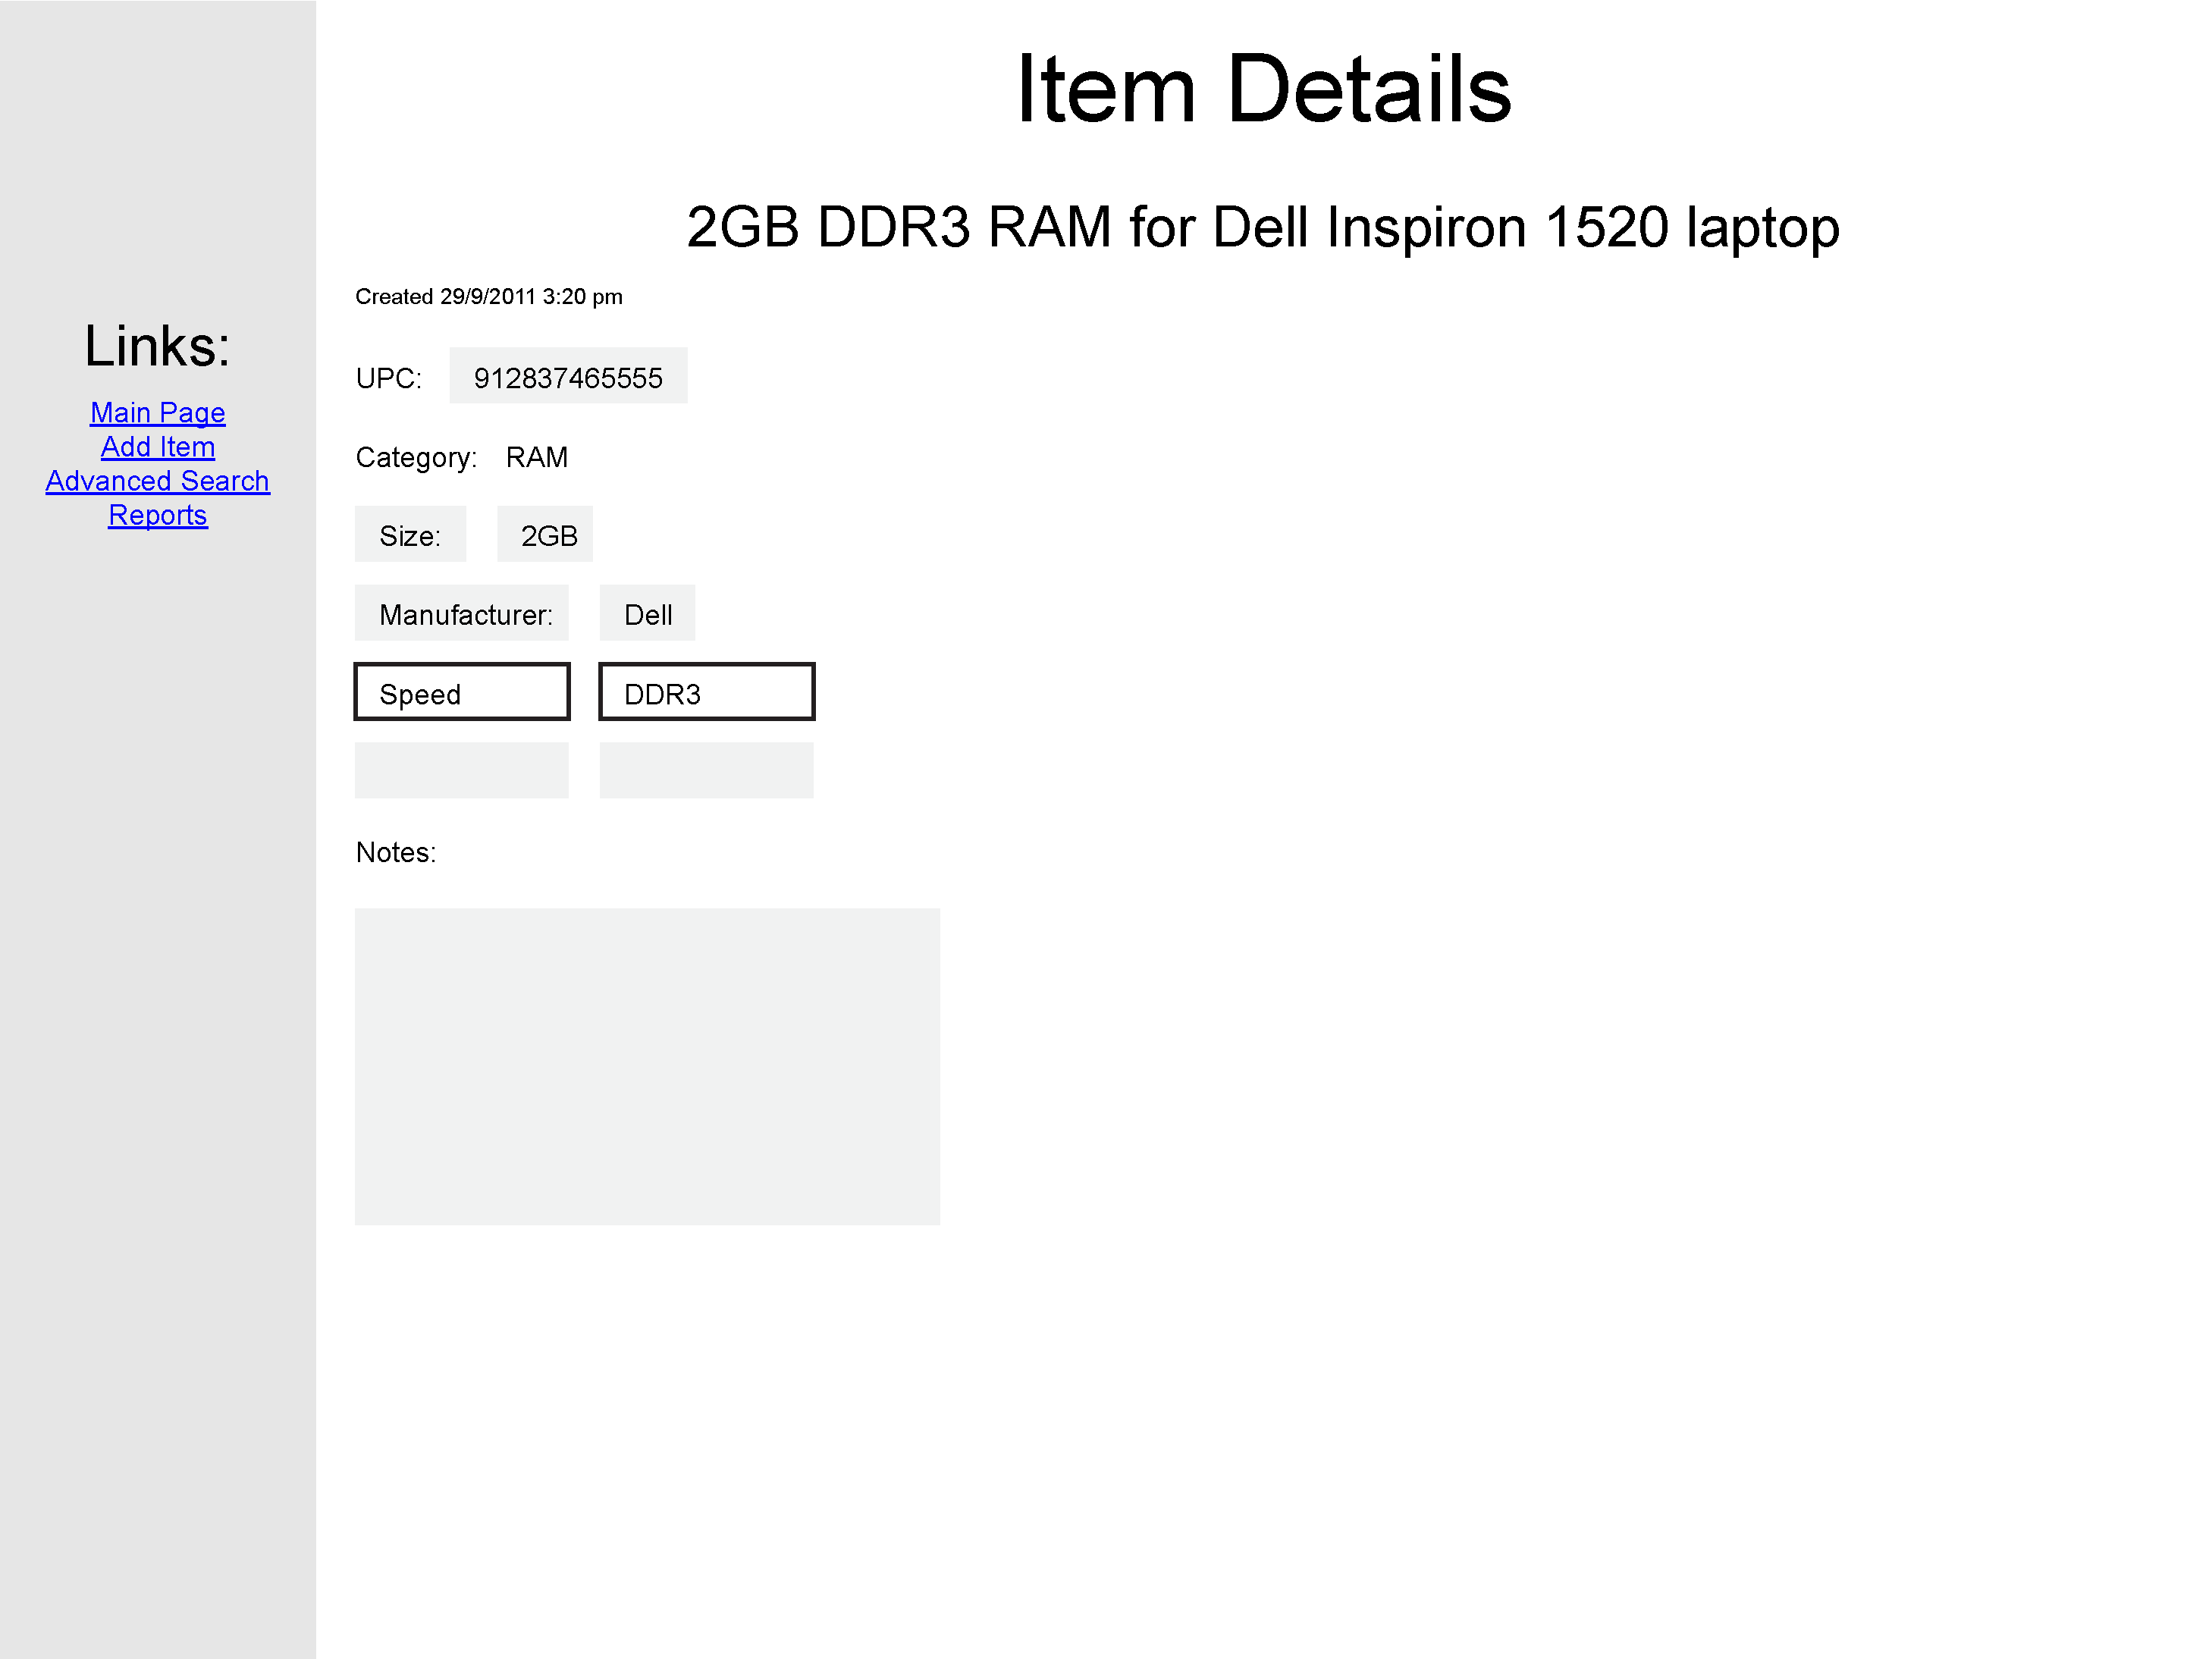
\includegraphics[keepaspectratio, width=4.5in]{modifyDetailsF0S3.pdf} \\
The item details page after the attribute key and value have been entered
\end{tabular}\\
~\\
~\\
\begin{tabular}{ p{4.5in} }
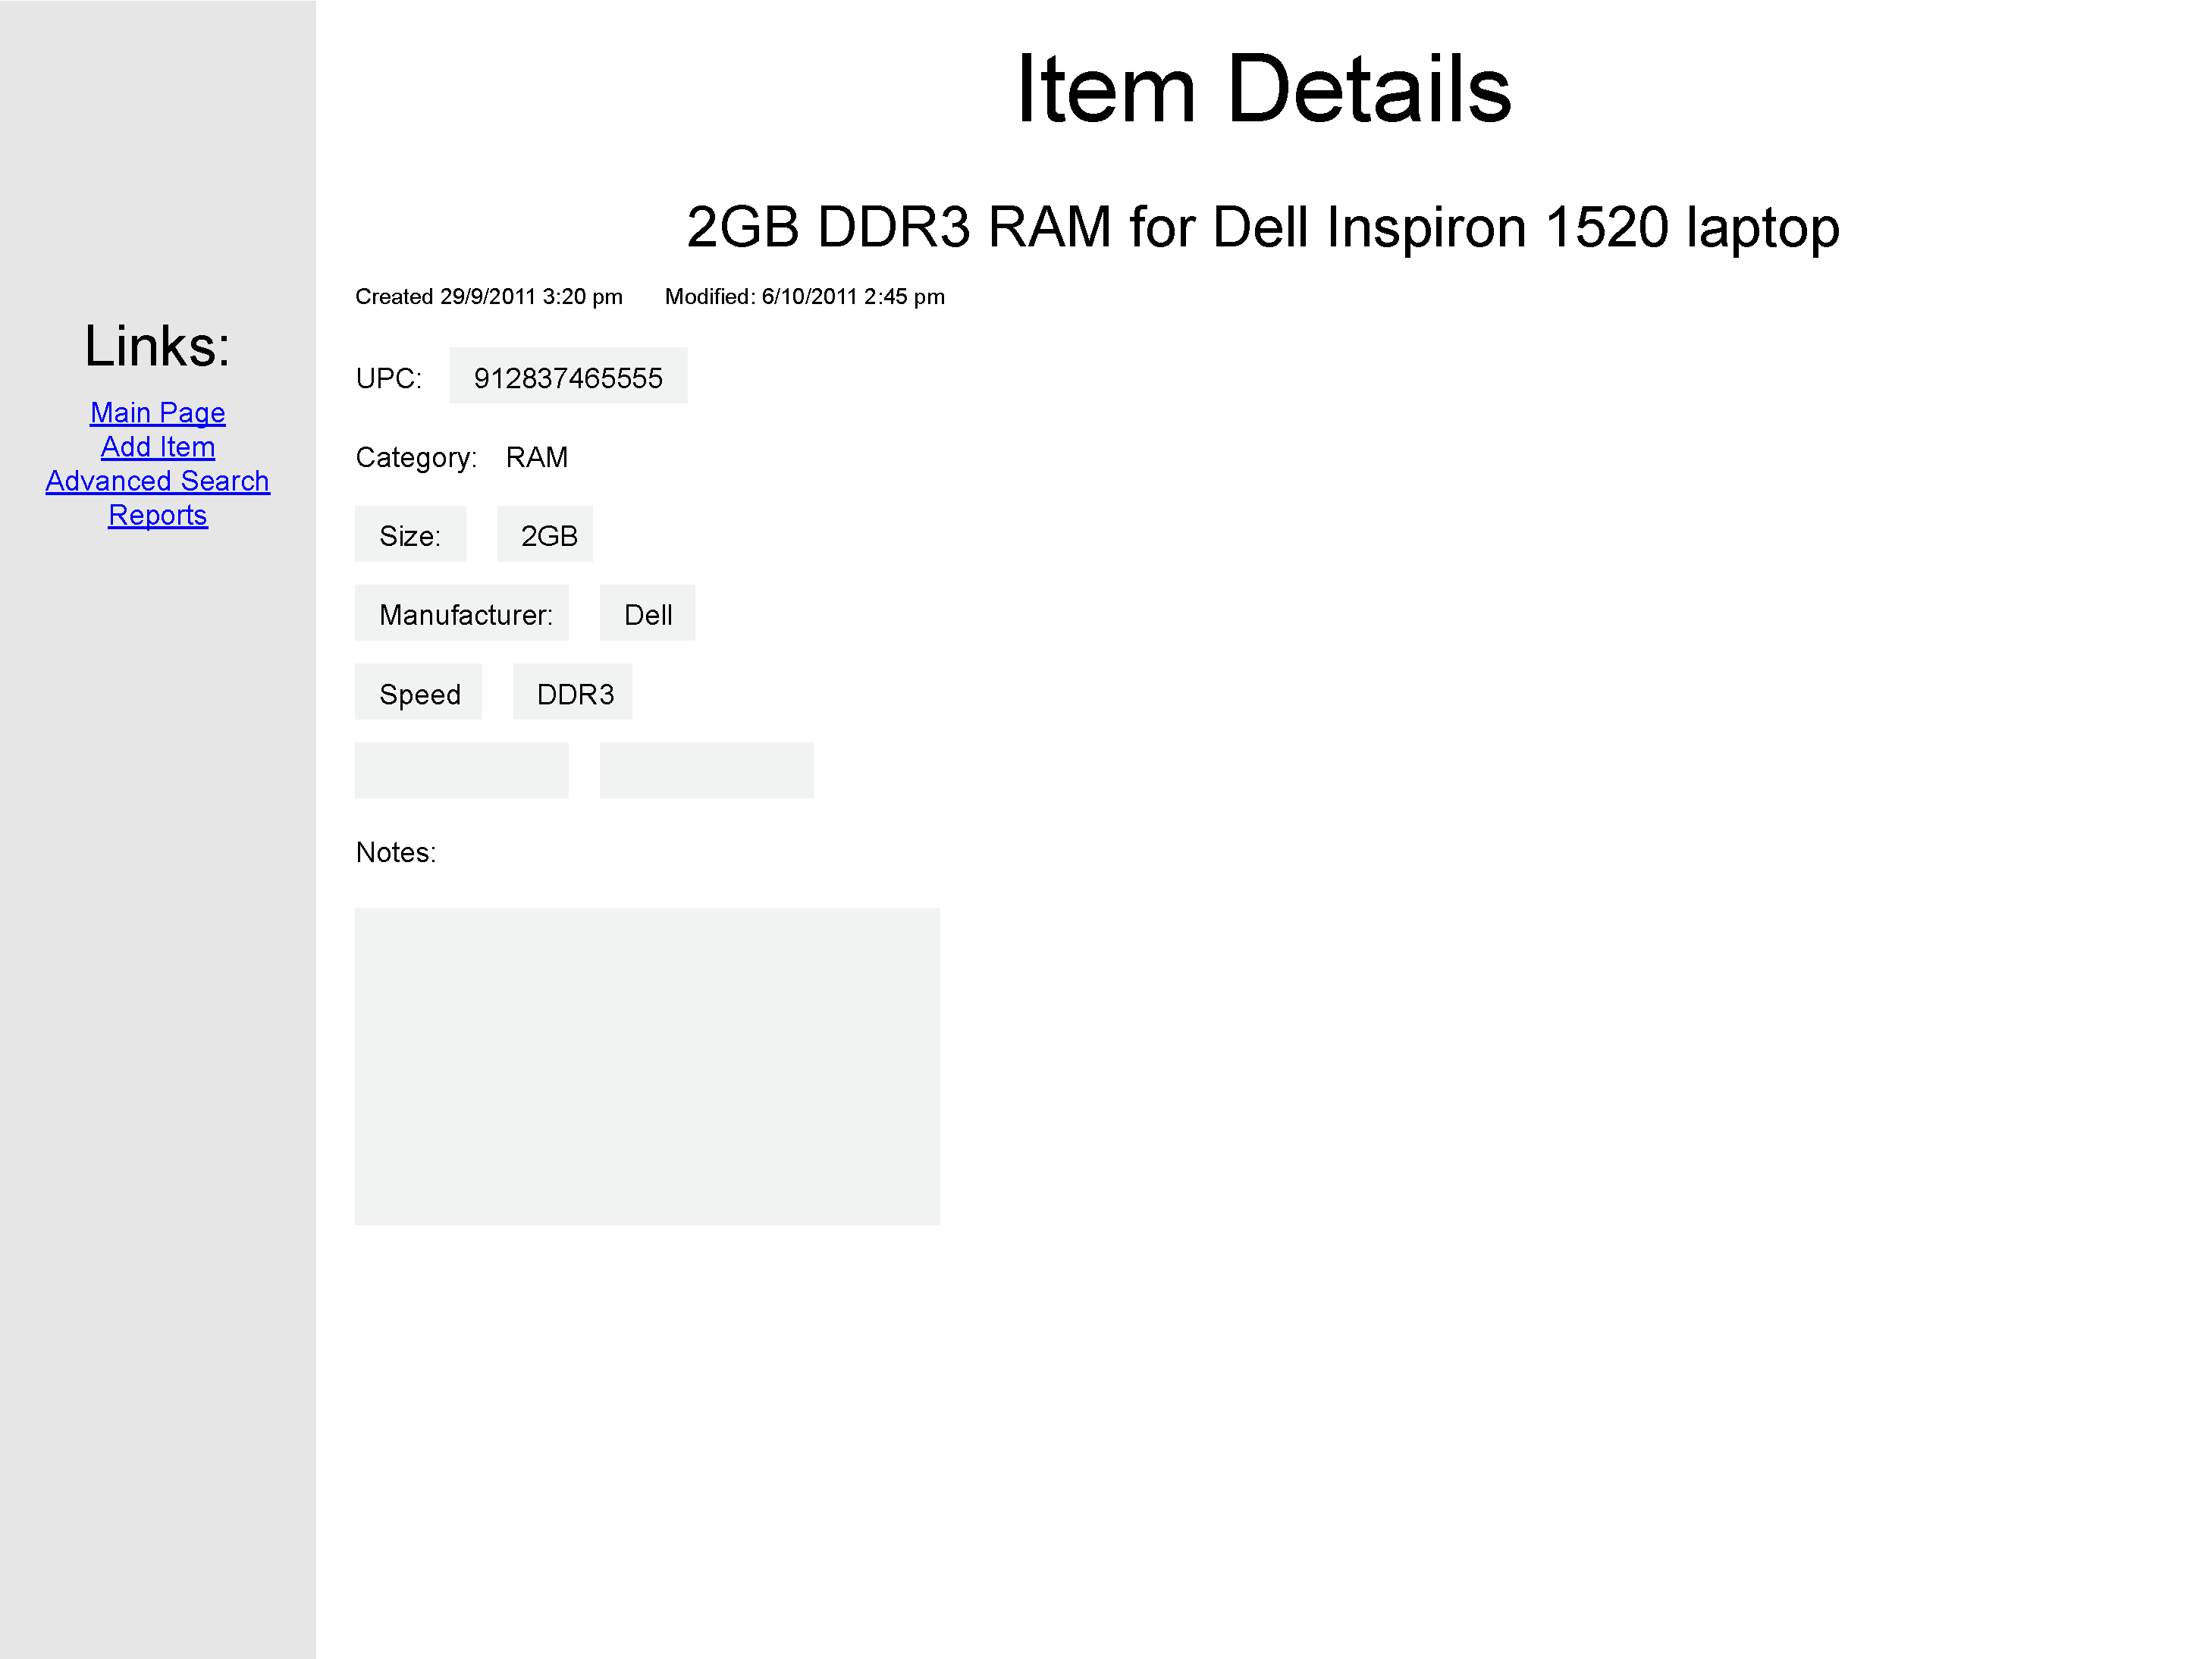
\includegraphics[keepaspectratio, width=4.5in]{modifyDetailsF0S4.pdf} \\
The item details page after the user has deselected the fields
\end{tabular}\\
~\\
~\\
\begin{tabular}{ p{4.5in} }
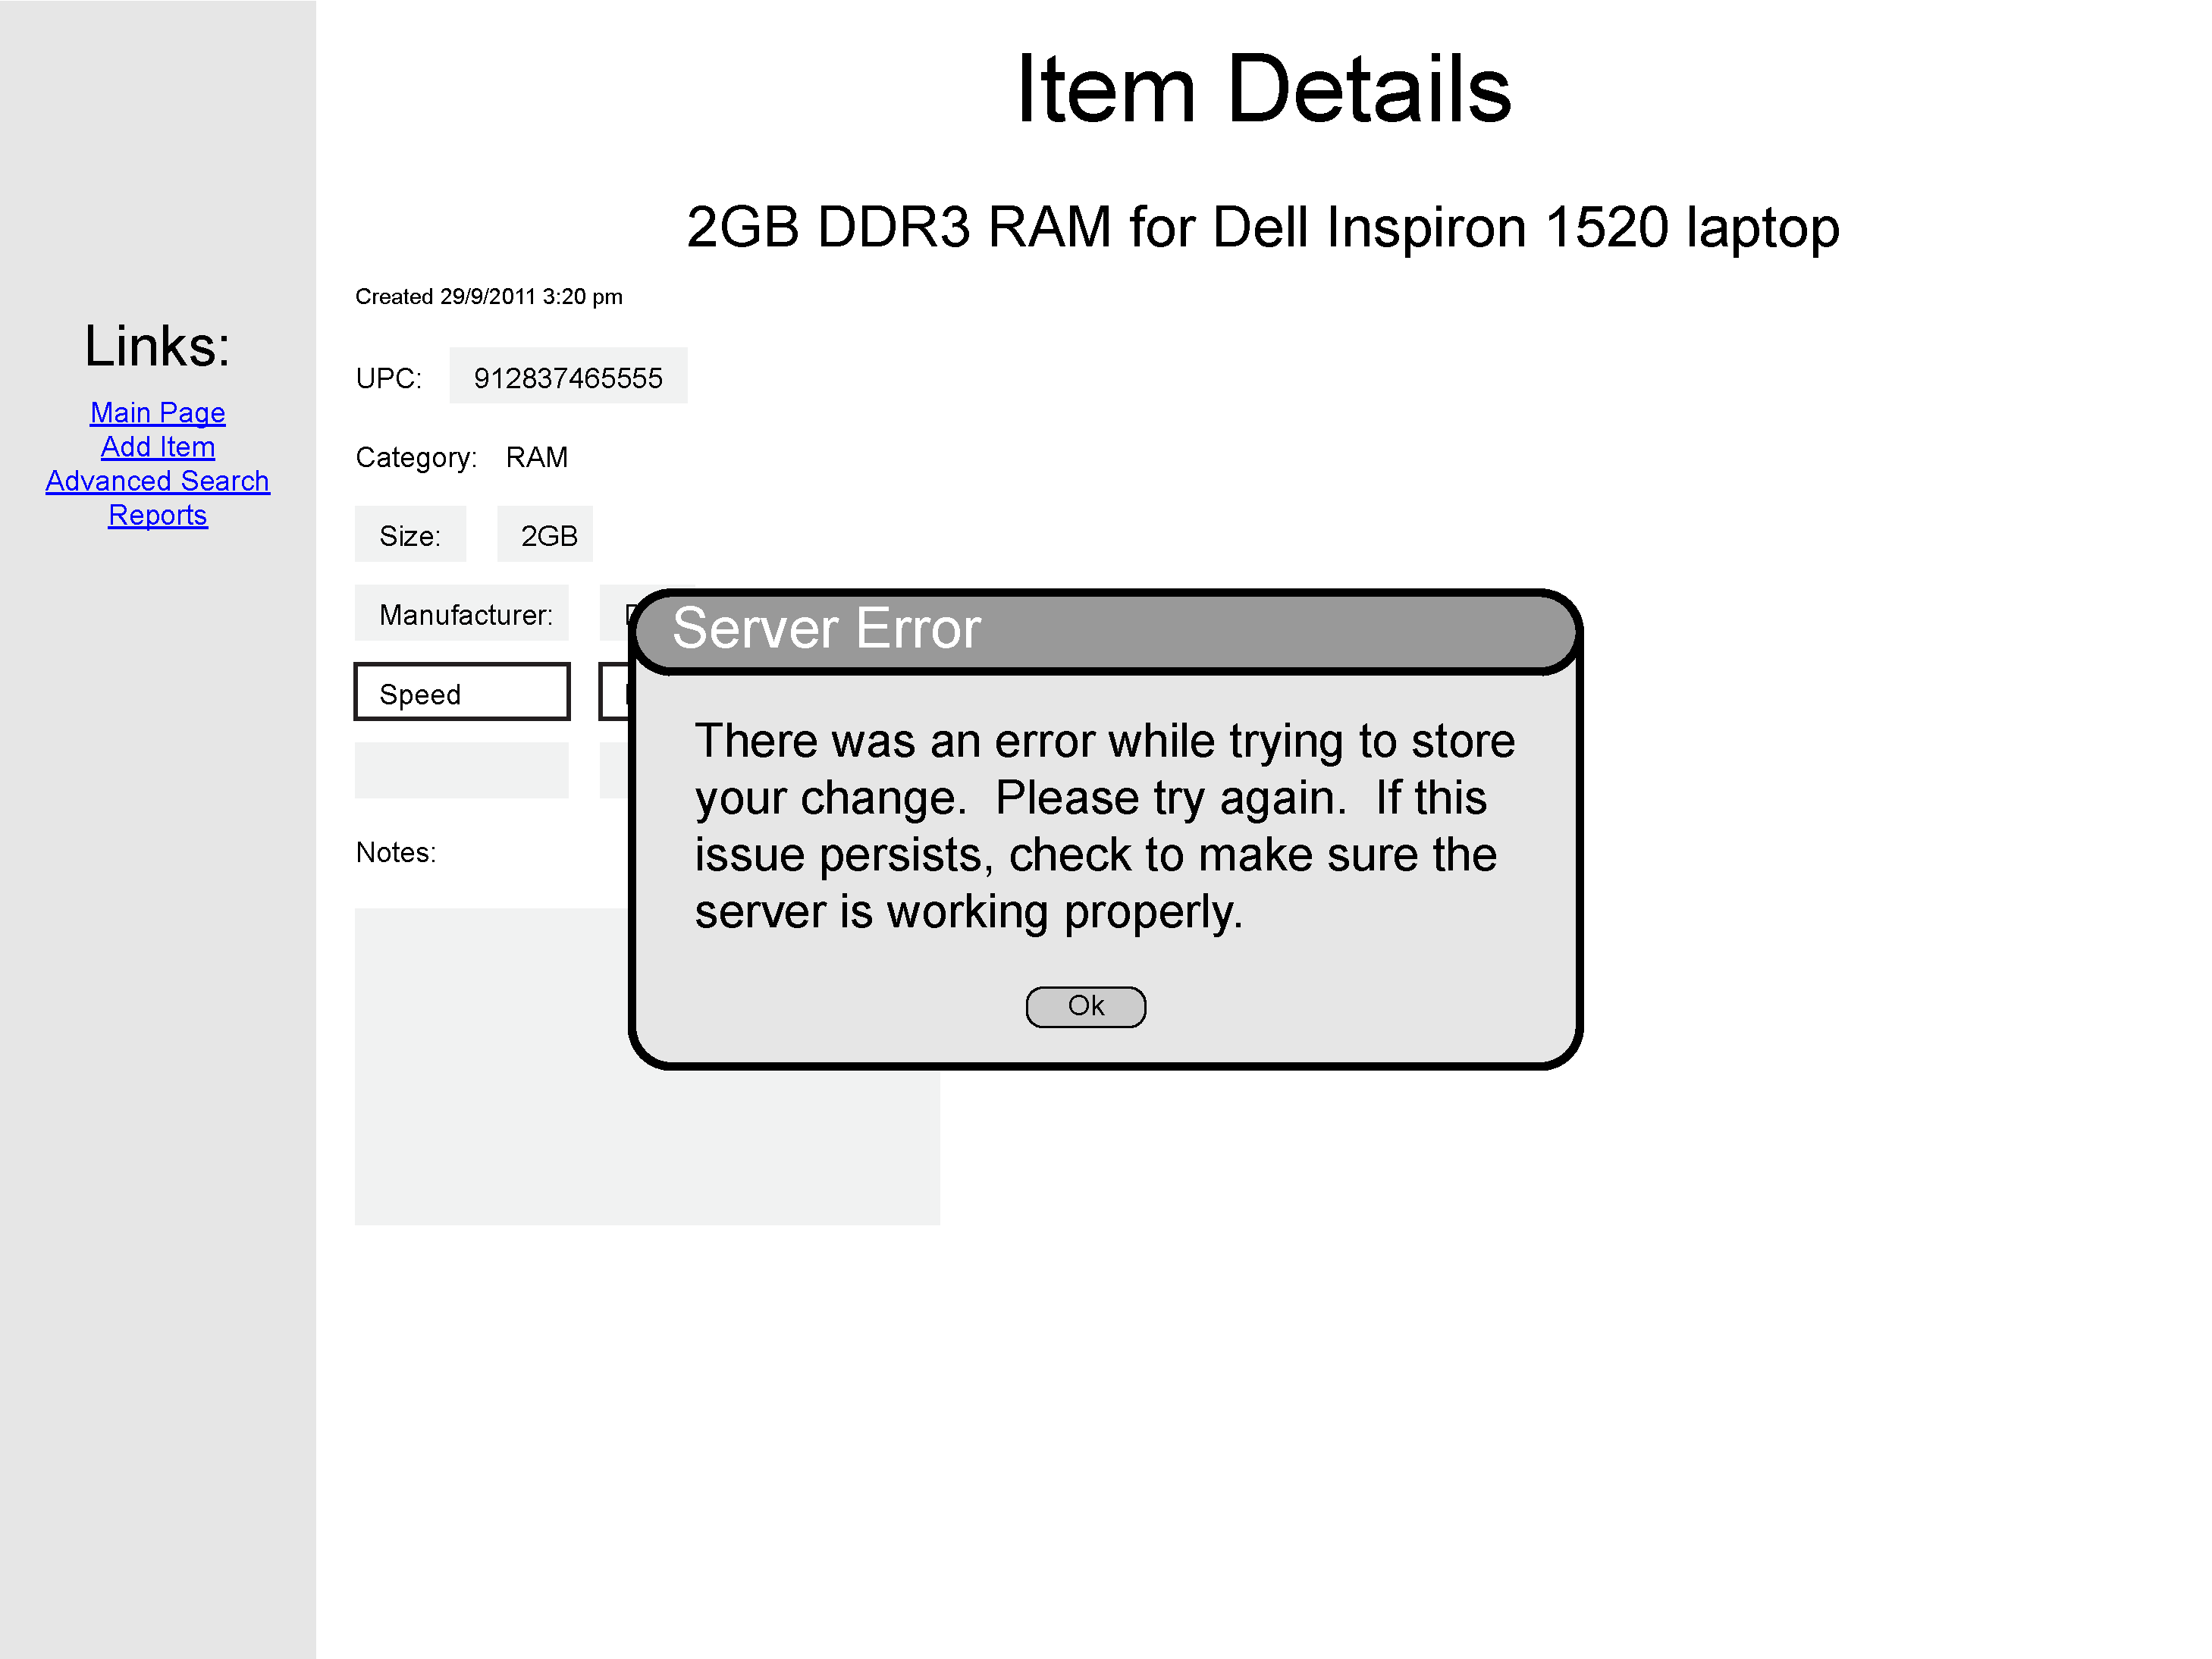
\includegraphics[keepaspectratio, width=4.5in]{modifyDetailsF1S4.pdf} \\
The item details page after the user has deselected the fields and the server has returned with an error
\end{tabular}\\
~\\
~\\
\begin{tabular}{ p{4.5in} }
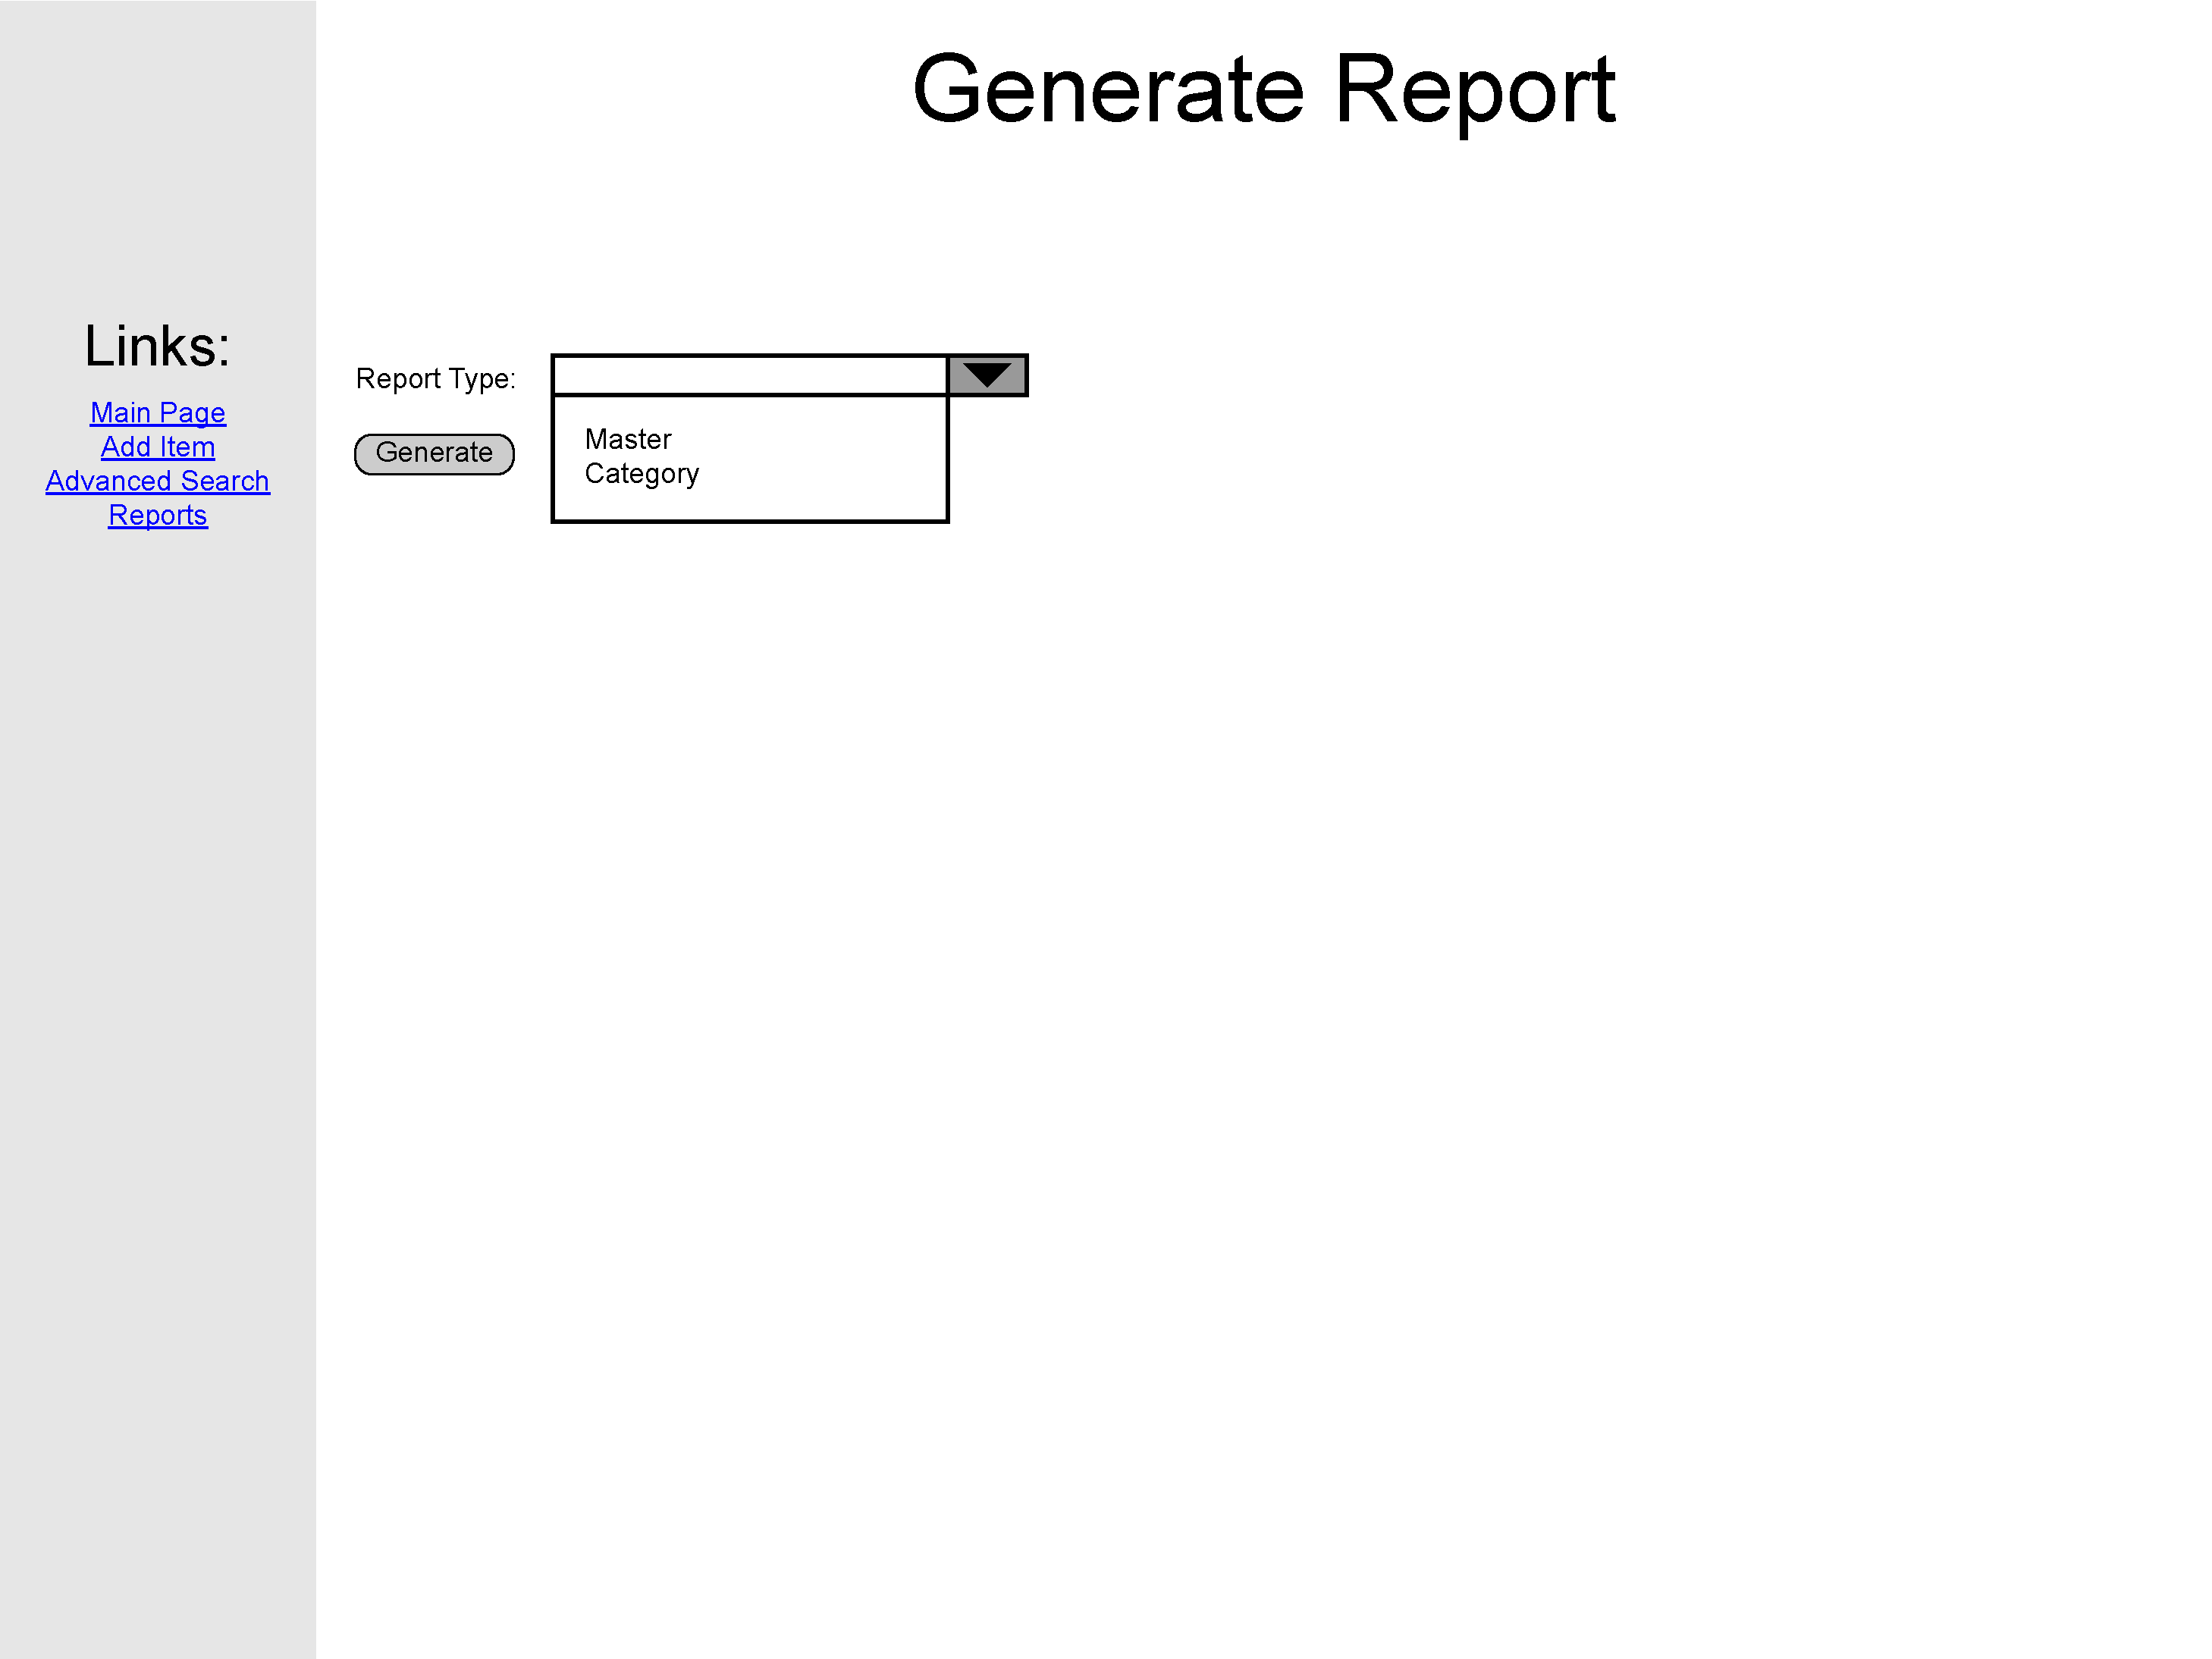
\includegraphics[keepaspectratio, width=4.5in]{generateReportF0S1.pdf} \\
The generate report page before a report type has been selected
\end{tabular}\\
~\\
~\\
\begin{tabular}{ p{4.5in} }
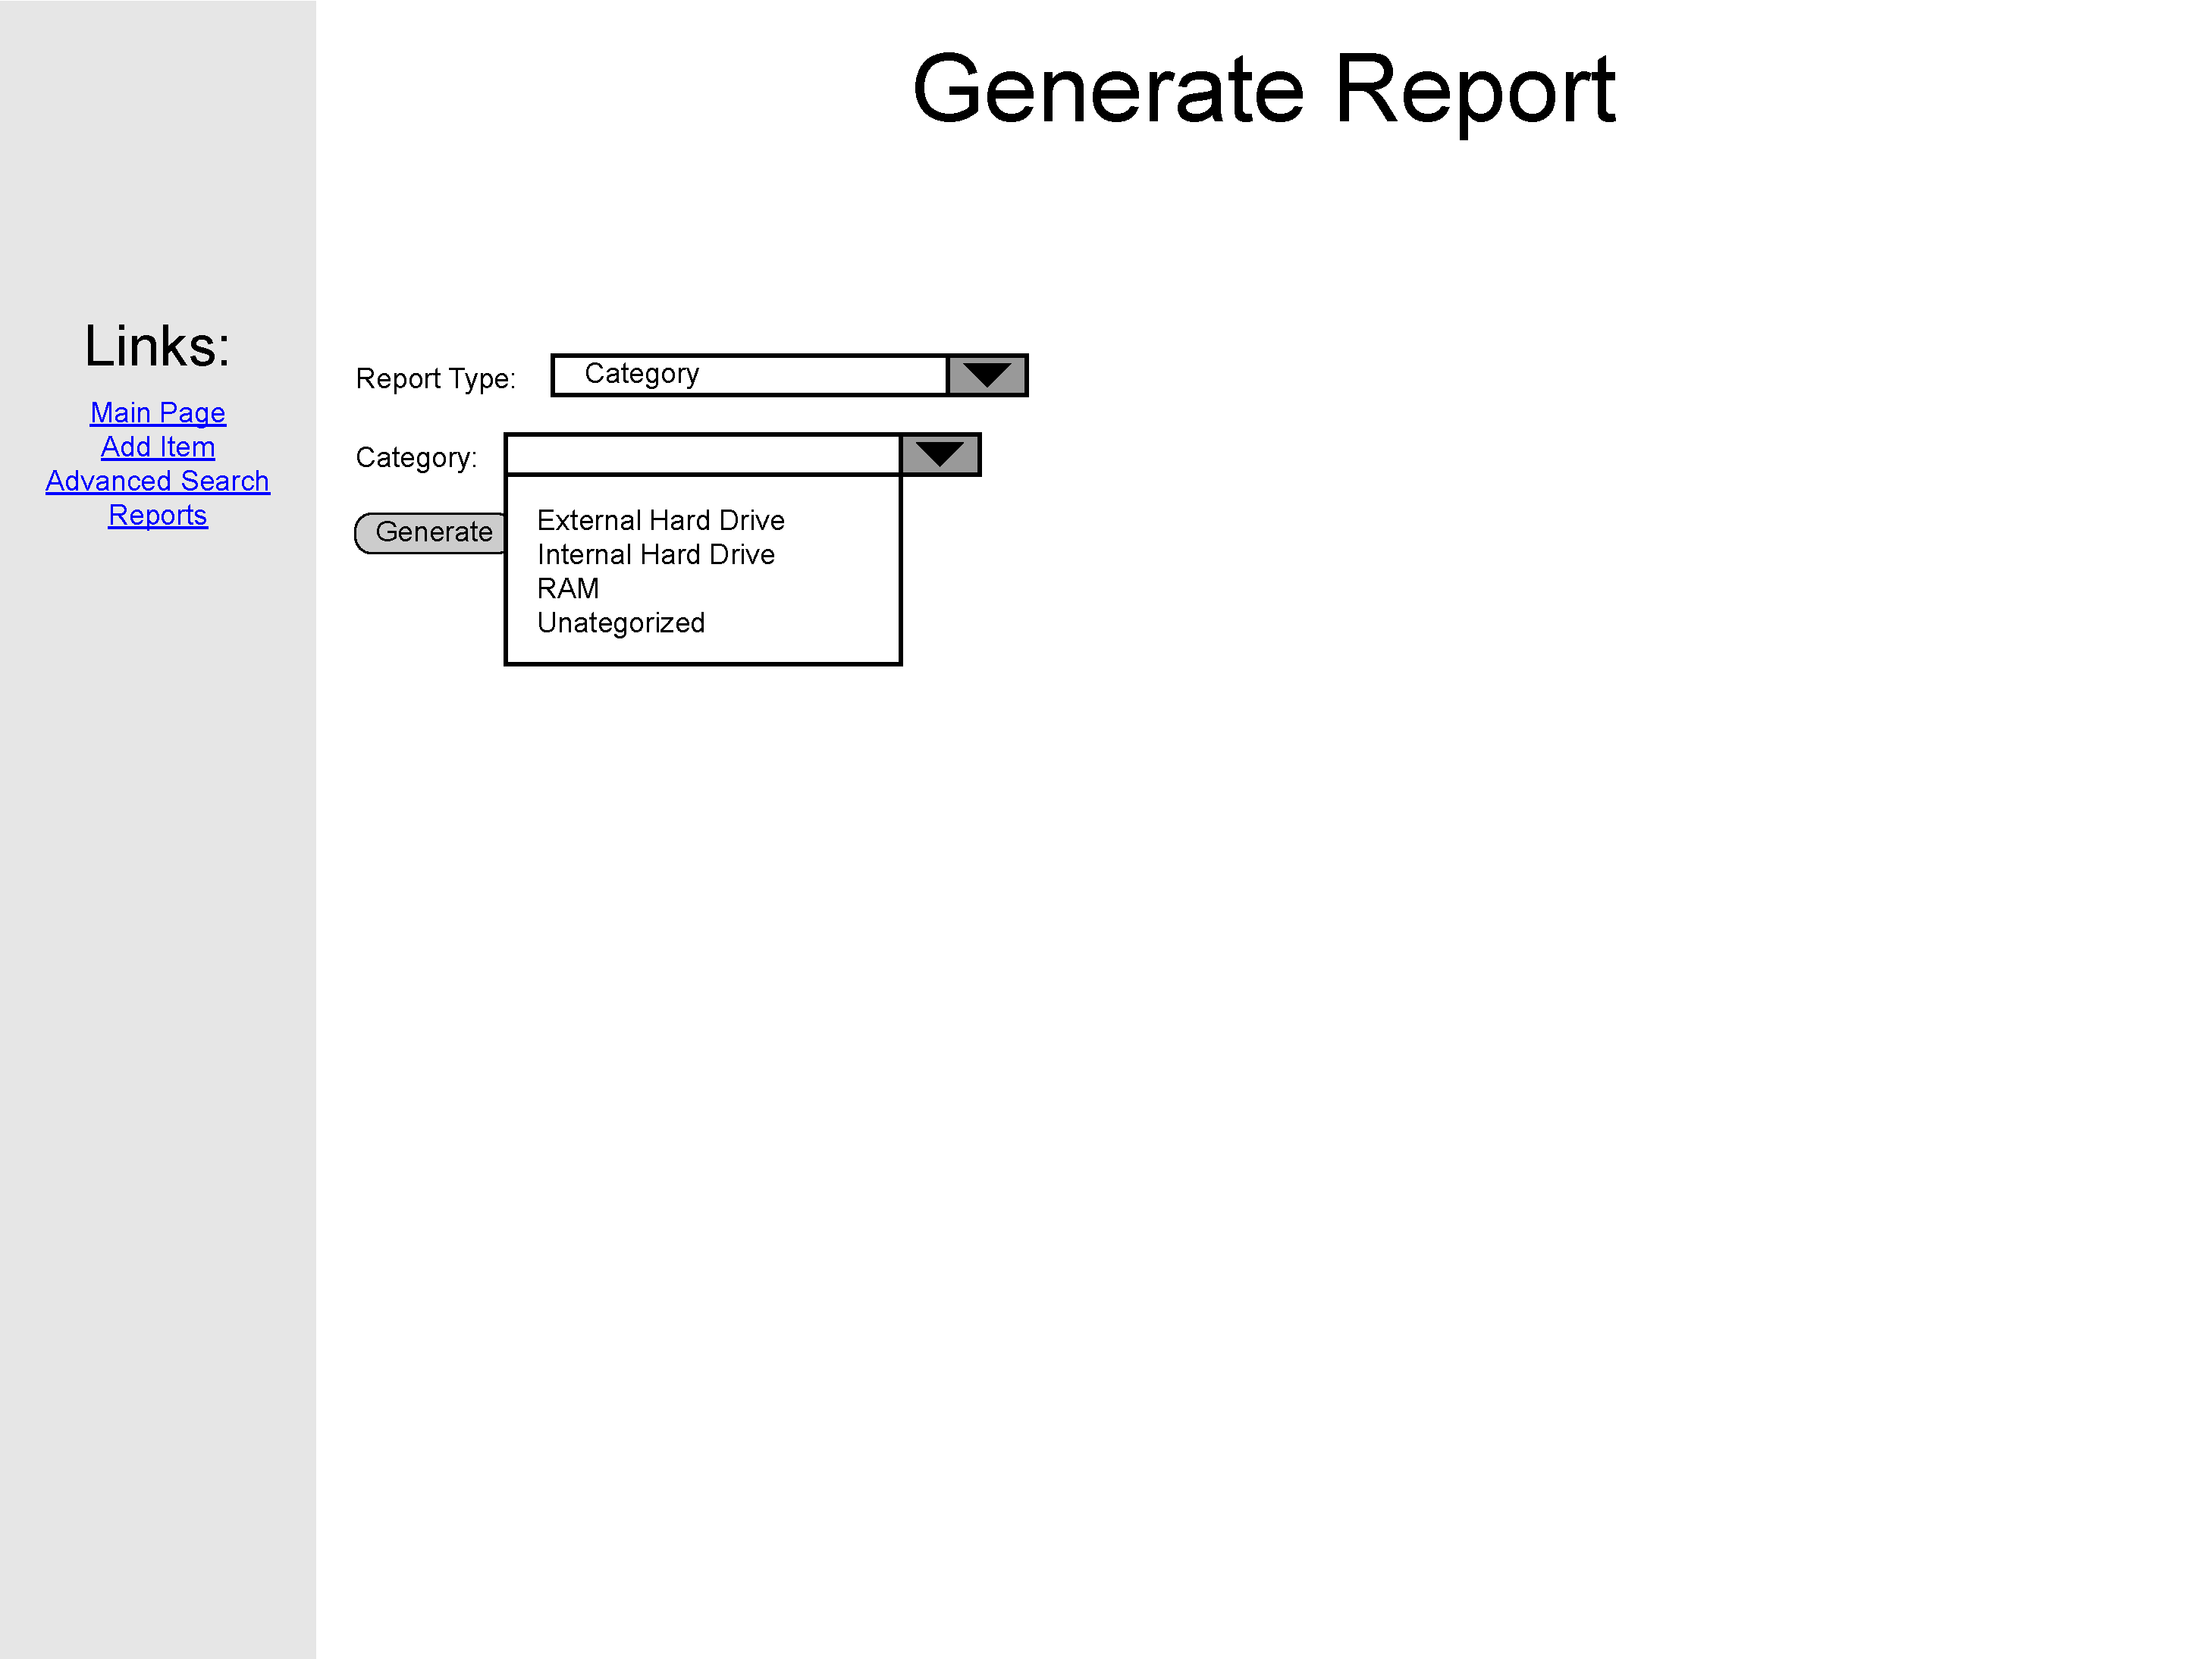
\includegraphics[keepaspectratio, width=4.5in]{generateReportF0S2.pdf} \\
The generate report page after the report type category has been selected, but before a category has been selected
\end{tabular}\\
~\\
~\\
\begin{tabular}{ p{4.5in} }
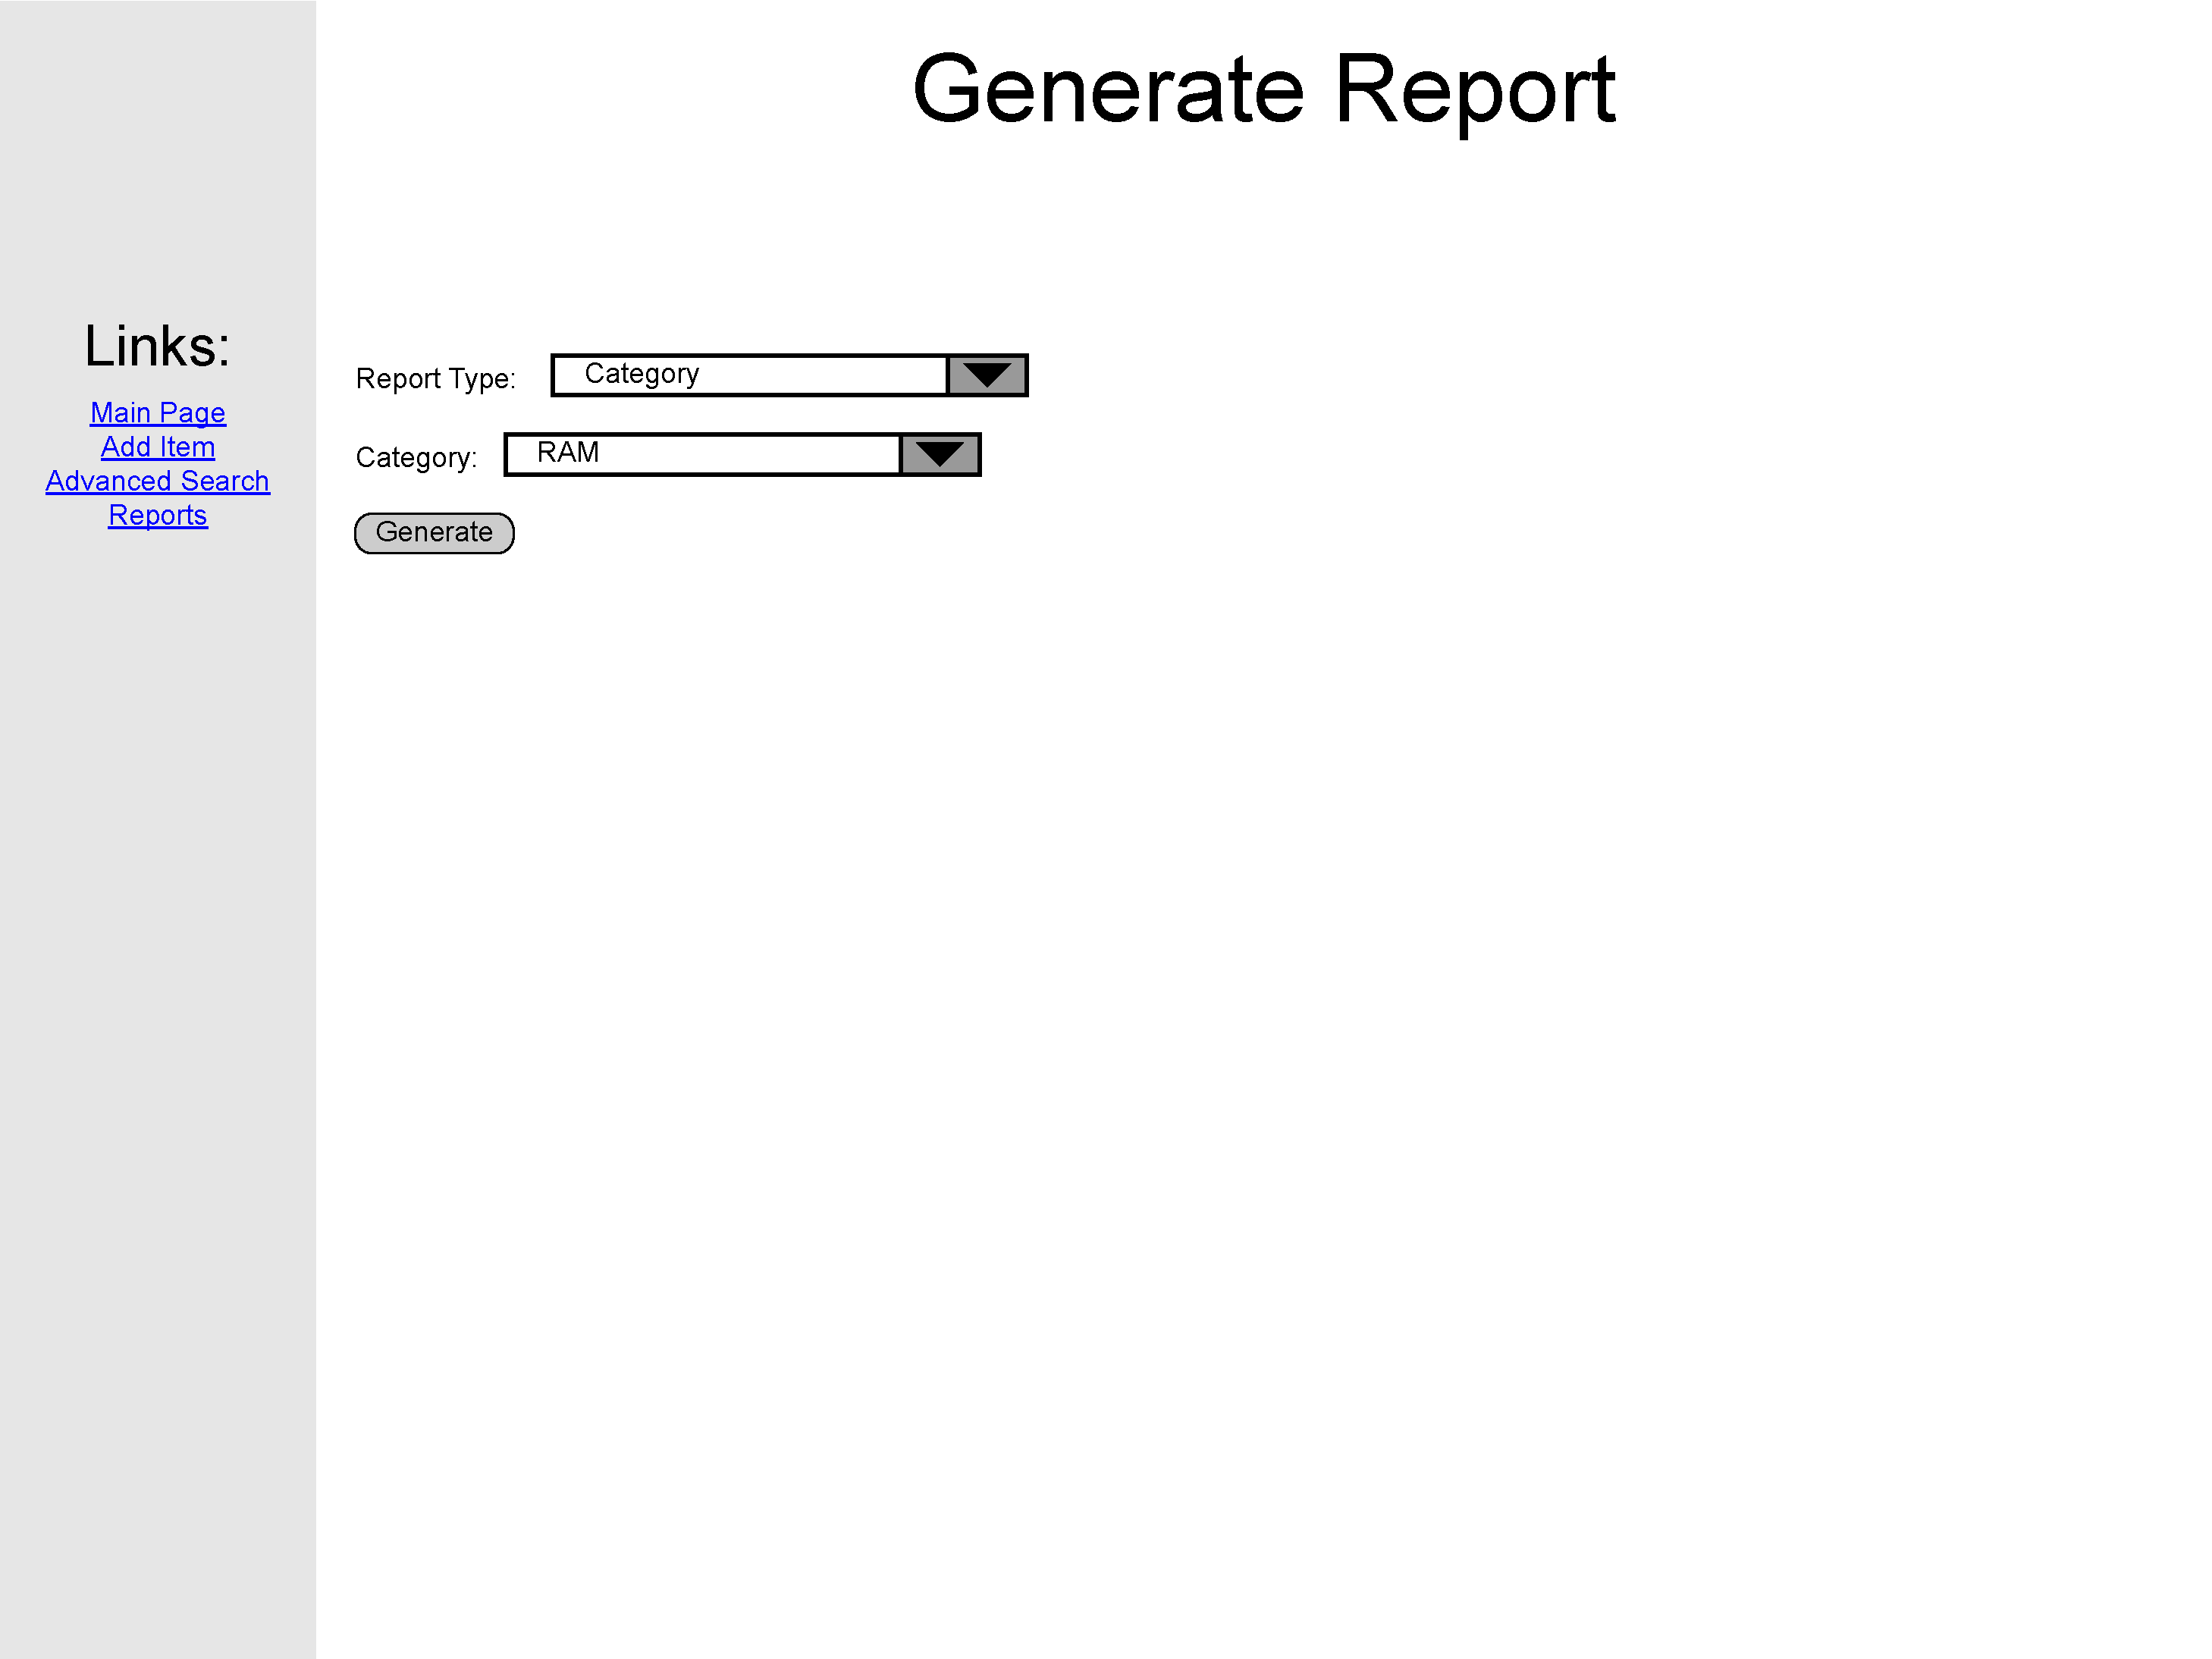
\includegraphics[keepaspectratio, width=4.5in]{generateReportF0S3.pdf} \\
The generate report page after the category of RAM has been selected
\end{tabular}\\
~\\
~\\
\begin{tabular}{ p{4.5in} }
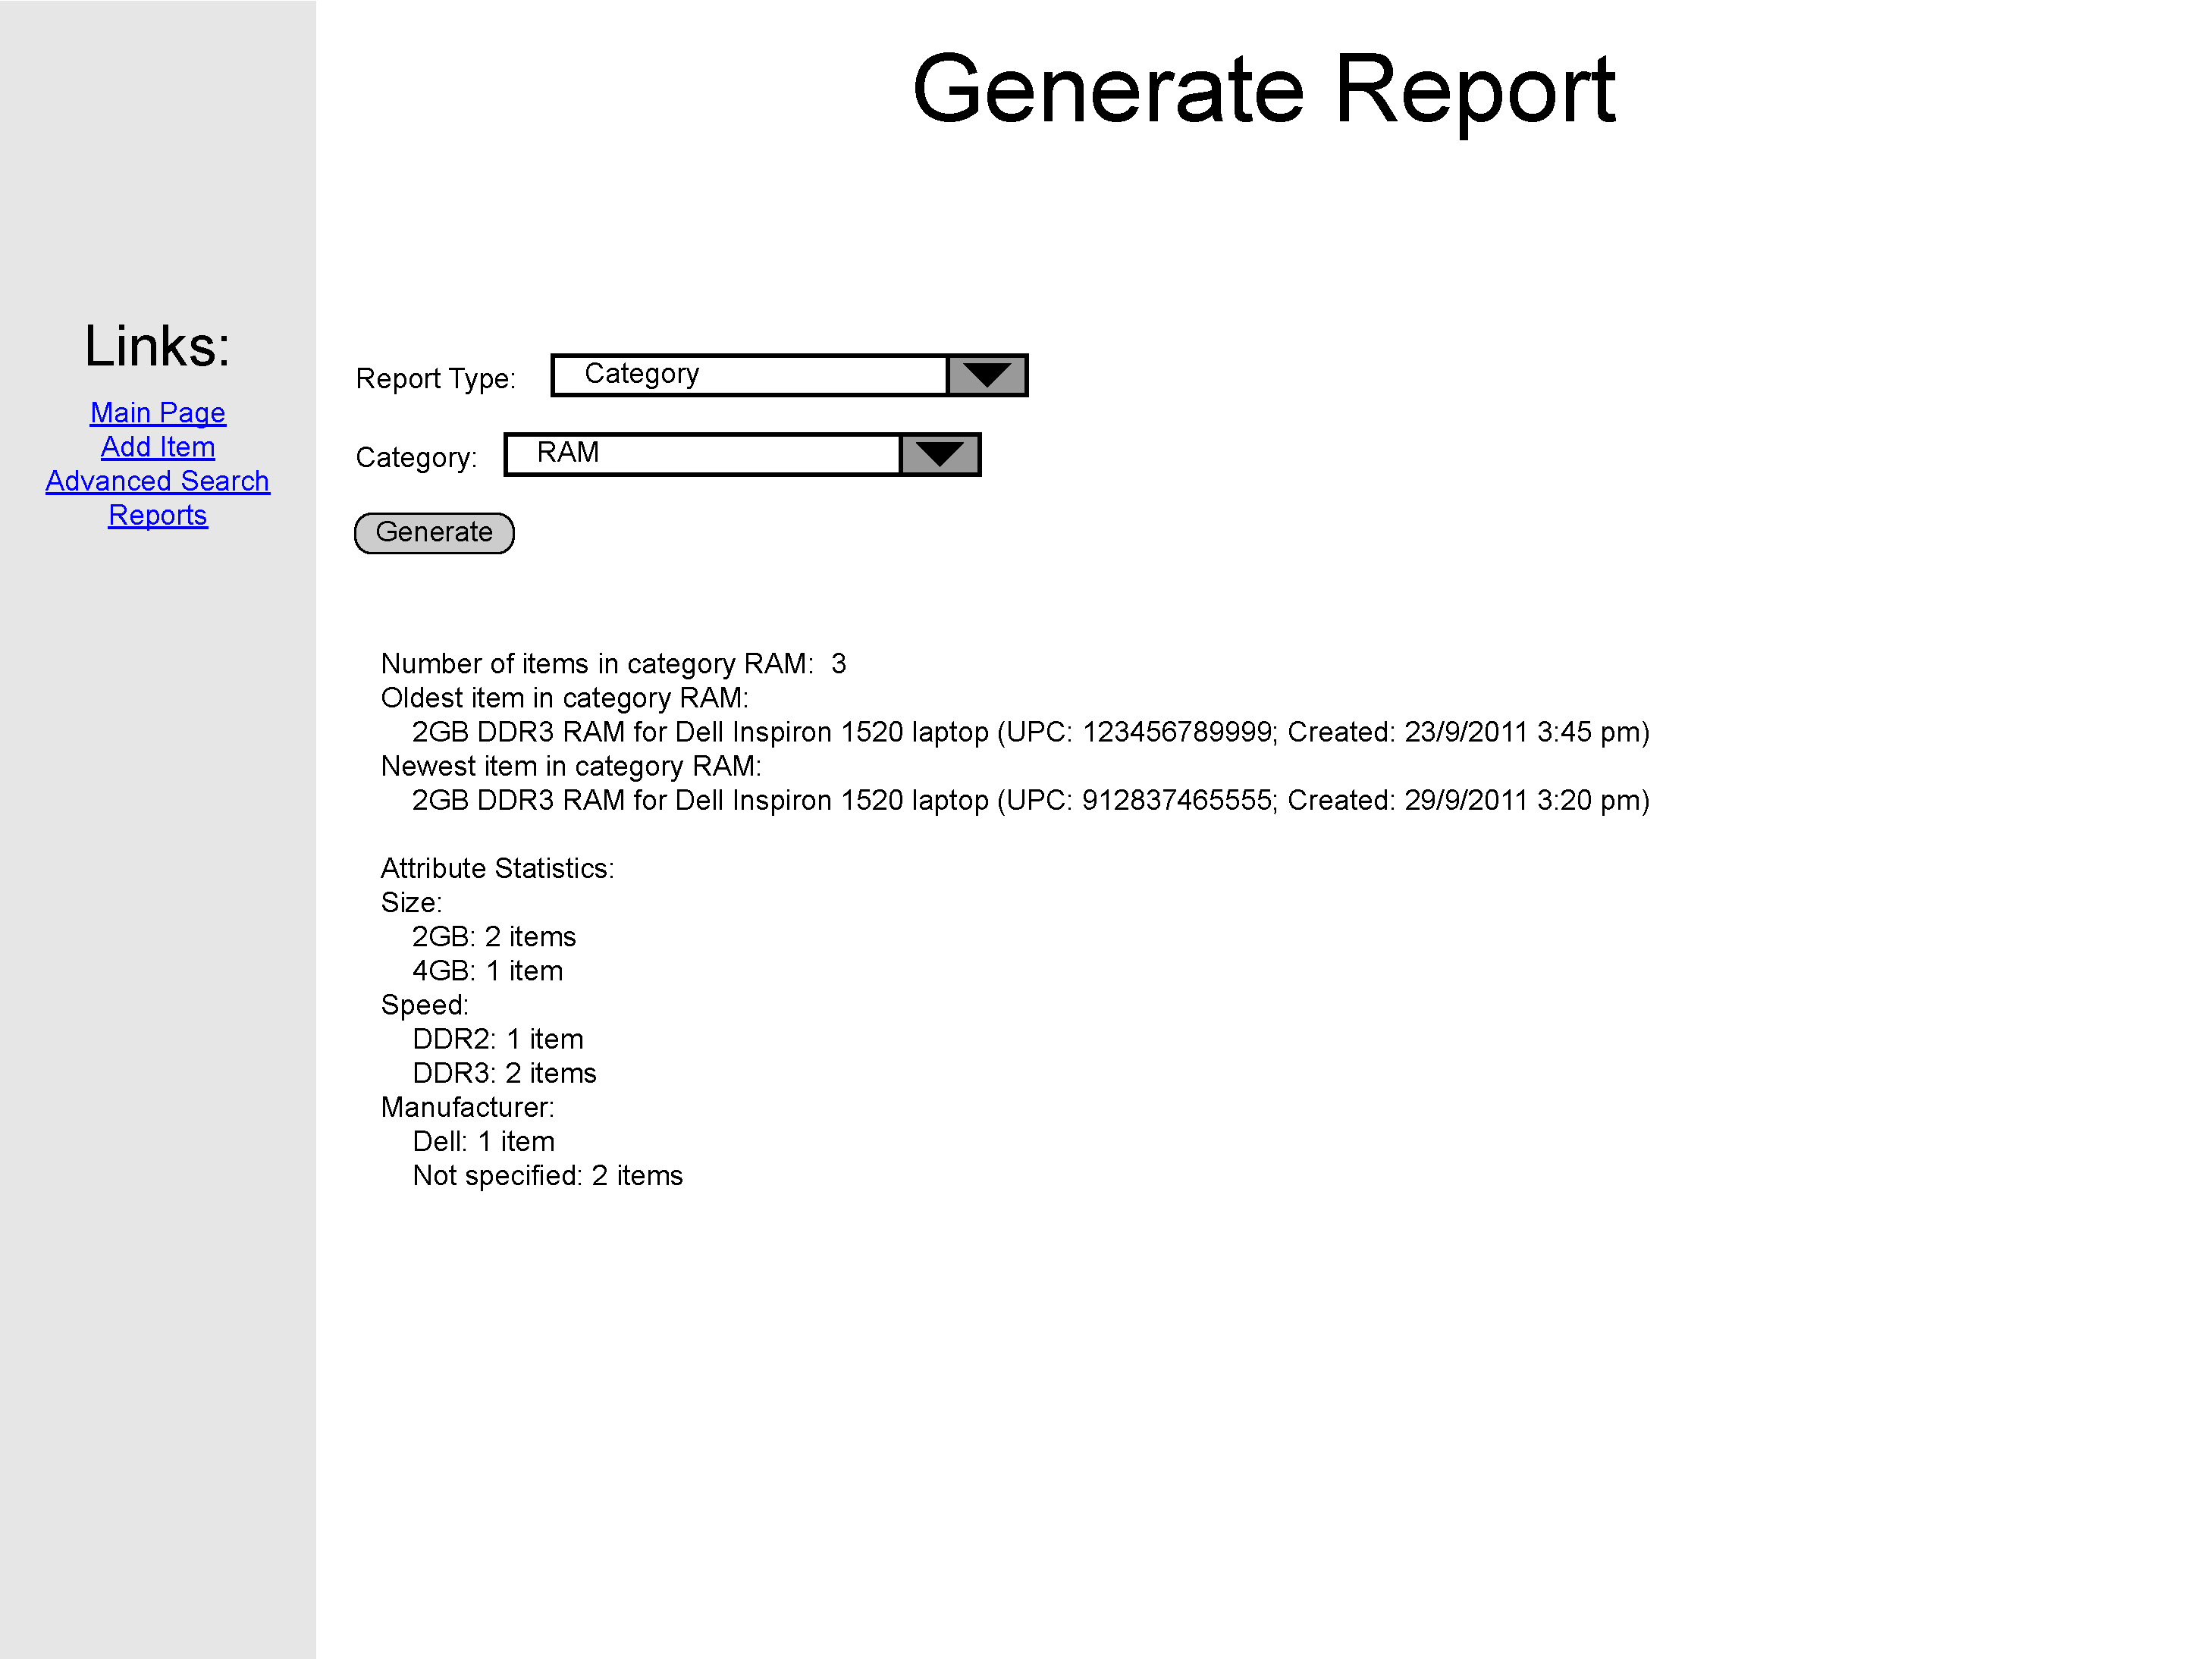
\includegraphics[keepaspectratio, width=4.5in]{generateReportF0S4.pdf} \\
The generate report page with the report being displayed
\end{tabular}

\section{Coding Standards}
\begin{itemize}
\item The code will use spaces, not tabs, to indent blocks
\item The code will use indentation increments of two spaces
\item The code will use underscores to separate words in variable names
\item The code will follow any other Ruby coding standards[14]
\item The folder structure for the product will be similar to that of the GasTracker project, a folder structure the client is familiar with
\end{itemize}

\section{Change Control}

\subsection{Receiving Requests}
If the client wishes to change the code, he will notify the team at a meeting.  Otherwise, he will fork the repository, make the changes himself, and submit a pull request.  If information is required for a change, it will be communicated either orally or via e-mail.  There will be no structured template for requesting changes, and more information will be requested if necessary.

\subsection{Managing Change and Source Control}
\begin{itemize}
\item Changes to sections carried over from previous milestones will be noted in a ``Deltas'' section, which has already been implemented in previous milestones
\item Changes to a milestone will be noted using the Git[13] change log
\item When content carried over from a previous milestone is changed, any milestones containing that content will be updated
\item Changes to anything in the repository will be noted with a detailed commit message
\item The source will be kept in a public repository on GitHub[13]
\end{itemize}

\section{Test Cases}
\label{test_case}

\paragraph{Test Case Syntax}
Each test case is divided into three sections:
\begin{itemize}
\item A ``Scenario Matrix'' section which describes each possible combination of flows (both basic and alternative) of a use case.
\item A ``Testing Matrix'' section which identifies distinct test cases defined by what conditions must be present in order to enact an expected result in response to the situation.
\item A ``Test Case to Scenario Matrix'' section which shows the correspondence between scenarios and test cases in order to help ensure completeness and traceability.
\end{itemize}

\subsection{Add an Item}
\textbf{NOTE:} Alternate Flow A0 will not be tested, since the server going offline is not an attribute of the system that can be measured.\label{flow}

\paragraph{Scenario Matrix}~\\ \\
\begin{tabular}{ c  c  c  c }
\hline
Scenario ID & Originating Flow & Alternate Flow & Next Alternate\label{scenario}\\
\hline
\hline
S0 & Basic &  & \\
\hline
S1 & Basic & A1 & \\
\hline
S2 & Basic & A2 & \\
\hline
S3 & Basic & A1 & A2\\
\hline
\end{tabular}\\
~\\
~\\
\paragraph{Testing Matrix}~\\ \\
\begin{tabular}{ p{0.8in}  p{0.7in}  p{0.7in}  p{3.3in} }
\hline
Test Case ID & Name Field & UPC Field & Expected Result\\
\hline
\hline
T0 & Present & Unique & The item is added successfully and the user is redirected to the main page with an updated Recent Changes list\\
\hline
T1 & Absent & Unique & The user is notified that a required field was omitted\\
\hline
T2 & Present & Absent & The user is notified that a required field was omitted\\
\hline
T3 & Absent & Absent & The user is notified that a required field was omitted\\
\hline
T4 & Present & Non-unique & The user is notified that the UPC is not unique\\
\hline
T5 & Absent & Non-unique & The user is notified that a required field was omitted and that the UPC is not unique\\
\hline
\end{tabular}\\
~\\
~\\
Present - a non-empty input\\
Absent - an empty input\\
Unique - a UPC code that is exclusive to the item\\
Non-unique - a UPC code that is no exclusive to the item
\paragraph{Test Case to Scenario Matrix}~\\ \\
\begin{tabular}{ | c || c | c | c | c | }
\hline
   & S0 & S1 & S2 & S3 \\
\hline
\hline
T0 & X  &    &    &    \\
\hline
T1 &    & X  &    &    \\
\hline
T2 &    & X  &    &    \\
\hline
T3 &    & X  &    &    \\
\hline
T4 &    &    & X  &    \\
\hline
T5 &    &    &    & X  \\
\hline
\end{tabular}

\subsection{Basic Search for an Item}
\textbf{NOTE:} Alternate Flow A1 will not be tested, since the server going offline is not an attribute of the system that can be measured.

\paragraph{Scenario Matrix}~\\ \\
\begin{tabular}{ c  c  c }
\hline
Scenario ID & Originating Flow & Alternate Flow\\
\hline
\hline
S4 & Basic &  \\
\hline
S5 & Basic & A0 \\
\hline
S6 & Basic & A2 \\
\hline
\end{tabular}\\
~\\
~\\
\paragraph{Testing Matrix}~\\ \\
\begin{tabular}{ p{0.8in}  p{0.75in}  p{0.5in}  p{3in} }
\hline
Test Case ID & Query Field & Matches & Expected Result\\
\hline
\hline
T6 & Present & Present & The results of the query are displayed on the page\\
\hline
T7 & Absent & & The user remains on the same page\\
\hline
T8 & Present & Absent & The text ``No results'' is displayed on the page\\
\hline
\end{tabular}\\
~\\
~\\
Present - a non-empty input\\
Absent - an empty input
\paragraph{Test Case to Scenario Matrix}~\\ \\
\begin{tabular}{ | c || c | c | c | }
\hline
   & S4 & S5 & S6 \\
\hline
\hline
T6 & X  &    &    \\
\hline
T7 &    & X  &    \\
\hline
T8 &    &    & X  \\
\hline
\end{tabular}


\subsection{Advanced Search for an Item}
\textbf{NOTE:} Alternate Flow A1 will not be tested, since the server going offline is not an attribute of the system that can be measured.

\paragraph{Scenario Matrix}~\\ \\
\begin{tabular}{ c  c  c  c }
\hline
Scenario ID & Originating Flow & Alternate Flow & Next Alternate \\
\hline
\hline
S7 & Basic &  & \\
\hline
S8 & Basic & A0 & \\
\hline
S9 & Basic & A0 & A2 \\
\hline
S10 & Basic & A0 & A3 \\
\hline
S11 & Basic & A3 &  \\
\hline
\end{tabular}\\
~\\
~\\
\paragraph{Testing Matrix}~\\ \\
\begin{tabular}{ p{0.8in}  p{0.5in} p{0.7in}  p{0.5in}  p{3in} }
\hline
Test Case ID & Category Field & Name/UPC Field & Matches & Expected Result\\
\hline
\hline
T9 & Present &  & Present & The results of the query are displayed on the page\\
\hline
T10 & Absent & Present & Present & The results of the query are displayed on the page\\
\hline
T11 & Absent & Absent &  & The user remains on the current page\\
\hline
T12 & Absent & Present & Absent & The text ``No results'' is displayed on the page\\
\hline
T13 & Present &  & Absent & The text ``No results'' is displayed on the page\\
\hline
\end{tabular}\\
~\\
~\\
Present - a non-empty input\\
Absent - an empty input
\paragraph{Test Case to Scenario Matrix}~\\ \\
\begin{tabular}{ | c || c | c | c | c | c | }
\hline
    & S7  & S8  & S9  & S10 & S11 \\
\hline
\hline
T9  &  X  &     &     &     &     \\
\hline
T10 &     &  X  &     &     &     \\
\hline
T11 &     &     &  X  &     &     \\
\hline
T12 &     &     &     &  X  &     \\
\hline
T13 &     &     &     &     &  X  \\
\hline
\end{tabular}

\subsection{Search Result Sorting}
\textbf{NOTE:} Alternate Flow A0 will not be tested, since the server going offline is not an attribute of the system that can be measured.
\paragraph{Scenario Matrix}~\\ \\
\begin{tabular}{ c  c }
\hline
Scenario ID & Originating Flow\\
\hline
\hline
S12 & Basic\\
\hline
\end{tabular}\\
~\\
~\\
\paragraph{Testing Matrix}~\\ \\
\begin{tabular}{ p{0.8in}  p{1.1in}  p{3.6in} }
\hline
Test Case ID & Sort Type Field & Expected Result\\
\hline
\hline
T14 & Name & The search results are sorted by the Name field\\
\hline
T15 & UPC & The search results are sorted by the UPC field\\
\hline
T16 & Recently Created & The search results are sorted by the Recently Created field\\
\hline
T17 & Recently Modified & The search results are sorted by the Recently Modified field\\
\hline
\end{tabular}\\
~\\
~\\
Name - a required field that serves as a label; sorting for this field is alphanumeric (ascending or descending)\\
UPC - a required field that serves as an unique identifier; sorting for this field is numeric (ascending or descending)\\
Recently Created - an automatically generated field that denotes the timestamp of when an item was added; sorting for this field is based on date and time (ascending or descending)\\
Recently Modified - an automatically generated field that denotes the timestamp of when an item was added or changed; sorting for this field is based on date and time (ascending or descending)
\paragraph{Test Case to Scenario Matrix}~\\ \\
\begin{tabular}{ | c || c | }
\hline
    & S12 \\
\hline
\hline
T14 &  X  \\
\hline
T15 &  X  \\
\hline
T16 &  X  \\
\hline
T17 &  X  \\
\hline
\end{tabular}

\subsection{View Details of an Item}
\textbf{NOTE:} Alternate Flow A0 will not be tested, since the server going offline is not an attribute of the system that can be measured.

\paragraph{Scenario Matrix}~\\ \\
\begin{tabular}{ c  c }
\hline
Scenario ID & Originating Flow\\
\hline
\hline
S13 & Basic\\
\hline
\end{tabular}\\
~\\
~\\
\paragraph{Testing Matrix}~\\ \\
\begin{tabular}{ p{0.8in}  p{3.4in} }
\hline
Test Case ID & Expected Result\\
\hline
\hline
T18 & The user is taken to a page showing all of the item details\\
\hline
\end{tabular}\\
~\\
~\\
\paragraph{Test Case to Scenario Matrix}~\\ \\
\begin{tabular}{ | c || c | }
\hline
    & S13 \\
\hline
\hline
T18 &  X  \\
\hline
\end{tabular}

\subsection{Edit Details of an Item}
\textbf{NOTE:} Alternate Flow A0 will not be tested, since the server going offline is not an attribute of the system that can be measured.
\paragraph{Scenario Matrix}~\\ \\
\begin{tabular}{ c  c  c }
\hline
Scenario ID & Originating Flow & Alternate Flow\\
\hline
\hline
S14 & Basic & \\
\hline
S15 & Basic & A1\\
\hline
\end{tabular}\\
~\\
~\\
\paragraph{Testing Matrix}~\\ \\
\begin{tabular}{ p{0.8in}  p{0.9in}  p{0.9in}  p{2.8in}}
\hline
Test Case ID & Name Field & UPC Field & Expected Result\\
\hline
\hline
T19 & Unchanged & Unchanged & The user is shown the item details page with the modified information\\
\hline
T20 & Valid Change & Unchanged & The user is shown the item details page with the modified information\\
\hline
T21 & Unchanged & Valid Change & The user is shown the item details page with the modified information\\
\hline
T22 & Valid Change & Valid Change & The user is shown the item details page with the modified information\\
\hline
T23 & Invalid Change & Unchanged & A pop-up with `Invalid Information' is shown\\
\hline
T24 & Invalid Change & Valid Change & A pop-up with `Invalid Information' is shown\\
\hline
T25 & Invalid Change & Invalid Change & A pop-up with `Invalid Information' is shown\\
\hline
T26 & Unchanged & Invalid Change & A pop-up with `Invalid Information' is shown\\
\hline
T27 & Valid Change & Invalid Change & A pop-up with `Invalid Information' is shown\\
\hline
\end{tabular}\\
~\\
~\\
Unchanged - the field was not modified\\
Valid Change (relative to Name Field) - the field was modified to be non-empty\\
Valid Change (relative to UPC Field) - the field was modified to be non-empty and unique\\
Invalid Change (relative to Name Field) - the field was modified to be empty\\
Invalid Change (relative to UPC Field) - the field was modified to be empty or non-unique
\paragraph{Test Case to Scenario Matrix}~\\ \\
\begin{tabular}{ | c || c | c | }
\hline
    & S14 & S15 \\
\hline
\hline
T19 &  X  &     \\
\hline
T20 &  X  &     \\
\hline
T21 &  X  &     \\
\hline
T22 &  X  &     \\
\hline
T23 &     &  X  \\
\hline
T24 &     &  X  \\
\hline
T25 &     &  X  \\
\hline
T26 &     &  X  \\
\hline
T27 &     &  X  \\
\hline
\end{tabular}

\subsection{Generate Inventory Report}
\textbf{NOTE:} Alternate Flow A0 will not be tested, since the server going offline is not an attribute of the system that can be measured.

\paragraph{Scenario Matrix}~\\ \\
\begin{tabular}{ c  c }
\hline
Scenario ID & Originating Flow \\
\hline
\hline
S16 & Basic \\
\hline
\end{tabular}\\
~\\
~\\
\paragraph{Testing Matrix}~\\ \\
\begin{tabular}{ p{0.8in}  p{2.2in} }
\hline
Test Case ID & Expected Result\\
\hline
\hline
T28 & The report is displayed on the page\\
\hline
\end{tabular}\\
~\\
~\\
\paragraph{Test Case to Scenario Matrix}~\\ \\
\begin{tabular}{ | c || c | }
\hline
    & S16  \\
\hline
\hline
T28 &  X  \\
\hline
\end{tabular}

\section{Index and Glossary}
\textbf{Assigned to}: Developer ultimately responsible for the implementation of a feature (\pageref{feature}).\\ \\
\textbf{Bug}: An error in a computer program. A critical bug is a bug that strongly affects important parts of a system (\pageref{bug}).\\ \\
\textbf{Context Flow Diagram}: the highest level of the DFD; it shows the entirety of the system. The next level of specification is level 0, followed by level 1, then level 2, and so on (\pageref{cfd}).\\ \\
\textbf{Data corruption}: Errors in data that introduce unintended changes to the data (\pageref{data_corruption}).\\ \\
\textbf{Data Flow Diagram (DFD)}: A diagram that details the data and signals that are passed between different processes and subprocesses of the system. If a particular process is complex enough to warrant it, a separate diagram may be made that shows the subprocesses within that process, and if any of them is sufficiently complex, the repetition of the diagramming at each level can occur as much as is necessary to explain the system in enough detail (\pageref{dfd}).\\ \\
\textbf{Degraded system}: The system becomes degraded if there are too many queries performed too quickly or if the amount of data needing to be searched through becomes too large. When the system is degraded, it may result in the system ceasing to function and requiring a reboot (\pageref{degrad_sys}).\\ \\
\textbf{Effort}: Expectation of the resources and time consumed for a feature (\pageref{feature}).\\ \\
\textbf{Exact Matching}: Valid search candidates are determined by strict equality with the search input(s) (\pageref{feature}).\\ \\
\textbf{Feature}: A system capability that fulfills a user need (\pageref{feature}).\\ \\
\textbf{Flow}: A particular series of ordered steps through a sequence of events in a use case (\pageref{flow}).\\ \\
\textbf{Fuzzy Matching}: Valid search candidates are determined based on similarity to the original search input(s) (\pageref{feature}).\\ \\
\textbf{Interface}: A point of interaction between systems, whether hardware or software, that allows the systems to communicate using some protocol (\pageref{interface}).\\ \\
\textbf{Performance}: The speed and efficiency of an operation, program, or system at a set of tasks (\pageref{performance}).\\ \\
\textbf{Post-condition}: An expectation of the system's state after the events in a use case occur (\pageref{post_cond}).\\ \\
\textbf{Pre-condition}: An assumption about the state of a system before a use case's events are followed (\pageref{pre_cond}).\\ \\
\textbf{Priority}: Description of how essential a feature is to the project (\pageref{feature}).\\ \\
\textbf{Reliability}: The ability of a system to function in a range of conditions for a period of time without failing to perform its tasks (\pageref{reliability}).\\ \\
\textbf{REST}: Stands for ``Representational state transfer;'' is a style software architecture often used in servers for simplicity and scalability. Amongst other aspects of REST, it is stateless. This means each request sent from the client of the server that uses REST to the server does not require any information from any previous requests. All information required to fulfill the request must be sent with the request (\pageref{rest}).\\ \\
\textbf{Risk}: Probability that a feature will instigate delays in the project (\pageref{feature}).\\ \\
\textbf{Scenario}: A possible permutation of a set of flows that lead from one flow to another (\pageref{scenario}).\\ \\
\textbf{SOAP}: Stands for ``Simple Object Access Protocol;'' is a protocol for exchanging structured information across a network (\pageref{soap}).\\ \\
\textbf{Stability}: Likelihood that the understanding of a feature will change (\pageref{feature}).\\ \\
\textbf{Supportability}: The ease with which a system can be fixed should it become broken or out of order (\pageref{support}).\\ \\
\textbf{Target Release}: Expected release iteration of a testable feature (\pageref{feature}).\\ \\
\textbf{Test Case}: Specifies what the expected result of a series of actions will have in a system (\pageref{test_case}).\\ \\
\textbf{Universal Product Code (UPC)}: a specific kind of barcode assign uniquely to each item in the server (\pageref{upc}).\\ \\
\textbf{Usability}: The ease with which one may use or learn to use a system (\pageref{usability}).\\ \\
\textbf{Use case}: A description of the steps performed by a user and system that leads the user towards a useful outcome (\pageref{use_case}).\\ \\
\textbf{Wildcard Matching}: Valid search candidates are determined based on adherence to the user's given search pattern (\pageref{feature}).\\ \\

\section{References}
\hangindent=1.4cm
\textbf{(1)} Leffingwell, Dean, and Don Widrig.
\emph{Managing Software Requirements: a Use Case Approach}.
Addison-Wesley, Boston,
2nd Edition,
2003.\\

\noindent\hangindent=1.4cm
\textbf{(2)} ``Ruby 1.9.2''
\emph{Download Ruby.} Ruby. Web.  6 October 2011. \\

\noindent\hangindent=1.4cm
\textbf{(3)} ``Sinatra 1.3.0''
\emph{Sinatra: Documentation.} Sinatra. Web.  6 October 2011.\\

\noindent\hangindent=1.4cm
\textbf{(4)} ``Ubuntu 11.04''
\emph{Download Ubuntu.} Ubuntu. Web.  6 October 2011.\\

\noindent\hangindent=1.4cm
\textbf{(5)} ``SQLite 3.7.8''
\emph{SQLite Download Page.} SQLite. Web.  6 October 2011.\\

\noindent\hangindent=1.4cm
\textbf{(6)} ``Cucumber 1.1.0''
\emph{cucumber/cucumber.} Cucumber. Web.  6 October 2011.\\

\noindent\hangindent=1.4cm
\textbf{(7)} ``RSpec 2.6.0''
\emph{RSpec Documentation.} Relish. Web.  6 October 2011.\\

\noindent\hangindent=1.4cm
\textbf{(8)} ``DataMapper 1.1.0''
\emph{DataMapper - Documentation.} DataMapper. Web.  6 October 2011.\\

\noindent\hangindent=1.4cm
\textbf{(9)} ``Google Chrome 14.0.8'' 
\emph{About Google Chrome.} Google. Web.  7 October 2011.\\

\noindent\hangindent=1.4cm
\textbf{(10)} ``Firefox 7.0.1''
\emph{Mozilla Firefox Web Browser - Free Download.} Mozilla. Web.  7 October 2011.\\

\noindent\hangindent=1.4cm
\textbf{(11)} ``Apache 2.2''
\emph{Apache HTTP Server Version 2.2 Documentation - Apache HTTP Server.} Apache. Web.  7 October 2011.\\

\noindent\hangindent=1.4cm
\textbf{(12)} ``BSD''
\emph{The FreeBSD Copyright.} The FreeBSD Project. Web. 18 October 2011.\\

\noindent\hangindent=1.4cm
\textbf{(13)} ``GitHub''
\emph{GitHub - Social Coding.} GitHub, Inc. Web. 28 October 2011.\\

\noindent\hangindent=1.4cm
\textbf{(14)} ``The Unofficial Ruby Usage Guide'' \emph{The Unofficial Ruby Usage Guide.} Caliban. 28 October 2011.\\

\end{document}